% Options for packages loaded elsewhere
% Options for packages loaded elsewhere
\PassOptionsToPackage{unicode}{hyperref}
\PassOptionsToPackage{hyphens}{url}
\PassOptionsToPackage{dvipsnames,svgnames,x11names}{xcolor}
%
\documentclass[
  letterpaper,
  DIV=11,
  numbers=noendperiod]{scrartcl}
\usepackage{xcolor}
\usepackage{amsmath,amssymb}
\setcounter{secnumdepth}{5}
\usepackage{iftex}
\ifPDFTeX
  \usepackage[T1]{fontenc}
  \usepackage[utf8]{inputenc}
  \usepackage{textcomp} % provide euro and other symbols
\else % if luatex or xetex
  \usepackage{unicode-math} % this also loads fontspec
  \defaultfontfeatures{Scale=MatchLowercase}
  \defaultfontfeatures[\rmfamily]{Ligatures=TeX,Scale=1}
\fi
\usepackage{lmodern}
\ifPDFTeX\else
  % xetex/luatex font selection
\fi
% Use upquote if available, for straight quotes in verbatim environments
\IfFileExists{upquote.sty}{\usepackage{upquote}}{}
\IfFileExists{microtype.sty}{% use microtype if available
  \usepackage[]{microtype}
  \UseMicrotypeSet[protrusion]{basicmath} % disable protrusion for tt fonts
}{}
\makeatletter
\@ifundefined{KOMAClassName}{% if non-KOMA class
  \IfFileExists{parskip.sty}{%
    \usepackage{parskip}
  }{% else
    \setlength{\parindent}{0pt}
    \setlength{\parskip}{6pt plus 2pt minus 1pt}}
}{% if KOMA class
  \KOMAoptions{parskip=half}}
\makeatother
% Make \paragraph and \subparagraph free-standing
\makeatletter
\ifx\paragraph\undefined\else
  \let\oldparagraph\paragraph
  \renewcommand{\paragraph}{
    \@ifstar
      \xxxParagraphStar
      \xxxParagraphNoStar
  }
  \newcommand{\xxxParagraphStar}[1]{\oldparagraph*{#1}\mbox{}}
  \newcommand{\xxxParagraphNoStar}[1]{\oldparagraph{#1}\mbox{}}
\fi
\ifx\subparagraph\undefined\else
  \let\oldsubparagraph\subparagraph
  \renewcommand{\subparagraph}{
    \@ifstar
      \xxxSubParagraphStar
      \xxxSubParagraphNoStar
  }
  \newcommand{\xxxSubParagraphStar}[1]{\oldsubparagraph*{#1}\mbox{}}
  \newcommand{\xxxSubParagraphNoStar}[1]{\oldsubparagraph{#1}\mbox{}}
\fi
\makeatother


\usepackage{longtable,booktabs,array}
\newcounter{none} % for unnumbered tables
\usepackage{calc} % for calculating minipage widths
% Correct order of tables after \paragraph or \subparagraph
\usepackage{etoolbox}
\makeatletter
\patchcmd\longtable{\par}{\if@noskipsec\mbox{}\fi\par}{}{}
\makeatother
% Allow footnotes in longtable head/foot
\IfFileExists{footnotehyper.sty}{\usepackage{footnotehyper}}{\usepackage{footnote}}
\makesavenoteenv{longtable}
\usepackage{graphicx}
\makeatletter
\newsavebox\pandoc@box
\newcommand*\pandocbounded[1]{% scales image to fit in text height/width
  \sbox\pandoc@box{#1}%
  \Gscale@div\@tempa{\textheight}{\dimexpr\ht\pandoc@box+\dp\pandoc@box\relax}%
  \Gscale@div\@tempb{\linewidth}{\wd\pandoc@box}%
  \ifdim\@tempb\p@<\@tempa\p@\let\@tempa\@tempb\fi% select the smaller of both
  \ifdim\@tempa\p@<\p@\scalebox{\@tempa}{\usebox\pandoc@box}%
  \else\usebox{\pandoc@box}%
  \fi%
}
% Set default figure placement to htbp
\def\fps@figure{htbp}
\makeatother


% definitions for citeproc citations
\NewDocumentCommand\citeproctext{}{}
\NewDocumentCommand\citeproc{mm}{%
  \begingroup\def\citeproctext{#2}\cite{#1}\endgroup}
\makeatletter
 % allow citations to break across lines
 \let\@cite@ofmt\@firstofone
 % avoid brackets around text for \cite:
 \def\@biblabel#1{}
 \def\@cite#1#2{{#1\if@tempswa , #2\fi}}
\makeatother
\newlength{\cslhangindent}
\setlength{\cslhangindent}{1.5em}
\newlength{\csllabelwidth}
\setlength{\csllabelwidth}{3em}
\newenvironment{CSLReferences}[2] % #1 hanging-indent, #2 entry-spacing
 {\begin{list}{}{%
  \setlength{\itemindent}{0pt}
  \setlength{\leftmargin}{0pt}
  \setlength{\parsep}{0pt}
  % turn on hanging indent if param 1 is 1
  \ifodd #1
   \setlength{\leftmargin}{\cslhangindent}
   \setlength{\itemindent}{-1\cslhangindent}
  \fi
  % set entry spacing
  \setlength{\itemsep}{#2\baselineskip}}}
 {\end{list}}
\usepackage{calc}
\newcommand{\CSLBlock}[1]{\hfill\break\parbox[t]{\linewidth}{\strut\ignorespaces#1\strut}}
\newcommand{\CSLLeftMargin}[1]{\parbox[t]{\csllabelwidth}{\strut#1\strut}}
\newcommand{\CSLRightInline}[1]{\parbox[t]{\linewidth - \csllabelwidth}{\strut#1\strut}}
\newcommand{\CSLIndent}[1]{\hspace{\cslhangindent}#1}



\setlength{\emergencystretch}{3em} % prevent overfull lines

\providecommand{\tightlist}{%
  \setlength{\itemsep}{0pt}\setlength{\parskip}{0pt}}



 


\KOMAoption{captions}{tableheading}
\makeatletter
\@ifpackageloaded{tcolorbox}{}{\usepackage[skins,breakable]{tcolorbox}}
\@ifpackageloaded{fontawesome5}{}{\usepackage{fontawesome5}}
\definecolor{quarto-callout-color}{HTML}{909090}
\definecolor{quarto-callout-note-color}{HTML}{0758E5}
\definecolor{quarto-callout-important-color}{HTML}{CC1914}
\definecolor{quarto-callout-warning-color}{HTML}{EB9113}
\definecolor{quarto-callout-tip-color}{HTML}{00A047}
\definecolor{quarto-callout-caution-color}{HTML}{FC5300}
\definecolor{quarto-callout-color-frame}{HTML}{acacac}
\definecolor{quarto-callout-note-color-frame}{HTML}{4582ec}
\definecolor{quarto-callout-important-color-frame}{HTML}{d9534f}
\definecolor{quarto-callout-warning-color-frame}{HTML}{f0ad4e}
\definecolor{quarto-callout-tip-color-frame}{HTML}{02b875}
\definecolor{quarto-callout-caution-color-frame}{HTML}{fd7e14}
\makeatother
\makeatletter
\@ifpackageloaded{caption}{}{\usepackage{caption}}
\AtBeginDocument{%
\ifdefined\contentsname
  \renewcommand*\contentsname{Table of contents}
\else
  \newcommand\contentsname{Table of contents}
\fi
\ifdefined\listfigurename
  \renewcommand*\listfigurename{List of Figures}
\else
  \newcommand\listfigurename{List of Figures}
\fi
\ifdefined\listtablename
  \renewcommand*\listtablename{List of Tables}
\else
  \newcommand\listtablename{List of Tables}
\fi
\ifdefined\figurename
  \renewcommand*\figurename{Figure}
\else
  \newcommand\figurename{Figure}
\fi
\ifdefined\tablename
  \renewcommand*\tablename{Table}
\else
  \newcommand\tablename{Table}
\fi
}
\@ifpackageloaded{float}{}{\usepackage{float}}
\floatstyle{ruled}
\@ifundefined{c@chapter}{\newfloat{codelisting}{h}{lop}}{\newfloat{codelisting}{h}{lop}[chapter]}
\floatname{codelisting}{Listing}
\newcommand*\listoflistings{\listof{codelisting}{List of Listings}}
\makeatother
\makeatletter
\makeatother
\makeatletter
\@ifpackageloaded{caption}{}{\usepackage{caption}}
\@ifpackageloaded{subcaption}{}{\usepackage{subcaption}}
\makeatother
\usepackage{bookmark}
\IfFileExists{xurl.sty}{\usepackage{xurl}}{} % add URL line breaks if available
\urlstyle{same}
\hypersetup{
  pdftitle={Power Analysis for Confirmatory Factor Analysis: A Practical Tutorial},
  pdfauthor={Pablo Rogers},
  pdfkeywords={Power Analysis, Confirmatory Factor Analysis, Structural
Equation Modeling, Monte Carlo Simulation, semPower, simsem},
  colorlinks=true,
  linkcolor={blue},
  filecolor={Maroon},
  citecolor={Blue},
  urlcolor={Blue},
  pdfcreator={LaTeX via pandoc}}


\title{Power Analysis for Confirmatory Factor Analysis: A Practical
Tutorial}
\usepackage{etoolbox}
\makeatletter
\providecommand{\subtitle}[1]{% add subtitle to \maketitle
  \apptocmd{\@title}{\par {\large #1 \par}}{}{}
}
\makeatother
\subtitle{Analytical and Simulation-Based Approaches}
\author{Pablo Rogers}
\date{2026-09-24}
\begin{document}
\maketitle
\begin{abstract}
This tutorial presents a pedagogical introduction to statistical power
analysis in Confirmatory Factor Analysis (CFA). Proper sample size
planning requires assessing the probability of detecting overall model
misfit, either through analytical methods or simulation-based
approaches. Standard analytical tools rely on asymptotic normal theory,
which can break down under non-normality or missing data. This tutorial
demonstrates both strategies --- analytical (using semPower with lavaan
syntax) and Monte Carlo simulation (using simsem) --- side by side,
using the WHOQOL-BREF four-factor model as a unifying case study. We
illustrate how simulation complements analytical calculations by
enabling researchers to evaluate parameter-level power, coverage, and
relative bias under realistic scenarios involving model
misspecification, missing data, and non-normal continuous indicators. We
argue that analytical methods provide a fast and theoretically grounded
starting point for sample size planning, while simulation-based
approaches allow those conclusions to be stress-tested against the
specific population structure, misspecification form, and data
conditions of the study at hand.
\end{abstract}


\section{Introduction}\label{sec-intro}

Statistical power in CFA is the probability of correctly rejecting a
misspecified model --- or of detecting a parameter of interest when it
is truly non-zero in the population (MacCallum et al., 1996). Despite
its importance, power is rarely reported in applied CFA work:
researchers frequently fall back on arbitrary rules of thumb linking
required sample size to the number of observed variables or estimated
parameters, rather than conducting formal prospective calculations
(Aguirre-Urreta et al., 2024; Wolf et al., 2013).

Two main paradigms address power analysis in CFA:

\begin{enumerate}
\def\labelenumi{\arabic{enumi}.}
\tightlist
\item
  \textbf{Analytical methods}: Rely on the non-central \(\chi^2\)
  distribution to determine the sample size required for detecting
  global or local model misfit, typically quantified through the RMSEA
  (Jak et al., 2021; MacCallum et al., 1996).
\item
  \textbf{Simulation-based methods}: Use Monte Carlo data generation to
  estimate power, bias, and coverage for specific parameters or overall
  fit indices across varying sample sizes, without relying on the
  asymptotic assumptions that constrain analytical solutions (Muthén \&
  Muthén, 2002; Pornprasertmanit et al., 2021).
\end{enumerate}

This document provides a comprehensive tutorial covering both paradigms:
analytical power analysis using the \texttt{semPower} package, and Monte
Carlo simulation using the \texttt{simsem} package (Moshagen \& Bader,
2024; Pornprasertmanit et al., 2021).

\begin{tcolorbox}[enhanced jigsaw, arc=.35mm, bottomrule=.15mm, bottomtitle=1mm, breakable, colback=white, colbacktitle=quarto-callout-note-color!10!white, colframe=quarto-callout-note-color-frame, coltitle=black, left=2mm, leftrule=.75mm, opacityback=0, opacitybacktitle=0.6, rightrule=.15mm, title=\textcolor{quarto-callout-note-color}{\faInfo}\hspace{0.5em}{Reproducibility Note}, titlerule=0mm, toprule=.15mm, toptitle=1mm]

For local development and computational convenience, simulations in this
tutorial use 1,500 replications. Production-quality applied research
should increase this to 5,000 or more. Results throughout this tutorial
therefore carry more sampling variability than would be expected in a
final study. All analytical and simulation parameters are centrally
defined in \texttt{helpers.R} and \texttt{models.R} in
\texttt{Scripts/DataAppendixScripts}.

\end{tcolorbox}

\section{The Running Example: WHOQOL-BREF Population CFA
Model}\label{sec-popmodel}

All power analyses in this tutorial are anchored in the World Health
Organization Quality of Life-BREF (WHOQOL-BREF) four-factor measurement
model (Lin \& Yao, 2022; {Mosqueira Taipe et al.}, 2026). Meaningful
power analysis requires an explicit population model --- a formal
representation of the ``true'' covariance structure from which data are
presumed to be generated (Feng \& Hancock, 2023). By grounding this
model in meta-analytic evidence rather than in arbitrary parameter
choices, we ensure that sample size targets reflect realistic
measurement conditions (Lin \& Yao, 2022; {Mosqueira Taipe et al.},
2026).

We specify four population variants to support sensitivity analyses:

\begin{enumerate}
\def\labelenumi{\arabic{enumi}.}
\tightlist
\item
  \textbf{Meta-analytic} (\texttt{popmodel}): Loadings and residual
  variances matching the pooled estimates from Lin \& Yao (2022).
\item
  \textbf{Naive} (\texttt{naivemodel}): A pessimistic baseline derived
  from the lowest reported reliability values per domain ({Mosqueira
  Taipe et al.}, 2026).
\item
  \textbf{Optimistic} (\texttt{optmodel}): A best-case scenario derived
  from the highest reported reliability values per domain ({Mosqueira
  Taipe et al.}, 2026).
\item
  \textbf{Misspecification} (\texttt{h1model}): A cross-loading model
  representing the alternative hypothesis \(H_1\), with three additional
  cross-loadings based on the meta-EFA results of Lin \& Yao (2022).
\end{enumerate}

\subsection{Population model}\label{population-model}

The primary population model (\texttt{popmodel}) operationalizes a
meta-analytic scenario based on Lin \& Yao (2022), whose pooled EFA
estimates across 16 international studies provide the factor loadings
(\(\lambda\)). Key features of this model are:

\begin{itemize}
\tightlist
\item
  \textbf{Interfactor correlations (\(\phi\))}: Fixed at \(0.20\), a
  conservative midpoint of the reported range \(0.08\)--\(0.31\) (Lin \&
  Yao, 2022).
\item
  \textbf{Residual covariance}: Items \(Q3\) and \(Q4\) share a residual
  covariance (\(r_{Q3, Q4 \mid \text{physical}} = 0.30\)), preserving
  the subfactor signal identified in the five-factor EFA solution (Lin
  \& Yao, 2022).
\item
  \textbf{Factor structure}: Item \(Q8\) is retained in the
  Environmental domain despite loading more strongly on the
  Psychological domain in the meta-EFA. This constitutes the null
  hypothesis (\(H_0\)) version of the population, strictly maintaining
  the original four-factor structure without cross-loadings.
\end{itemize}

\begin{figure}[H]

\centering{

\pandocbounded{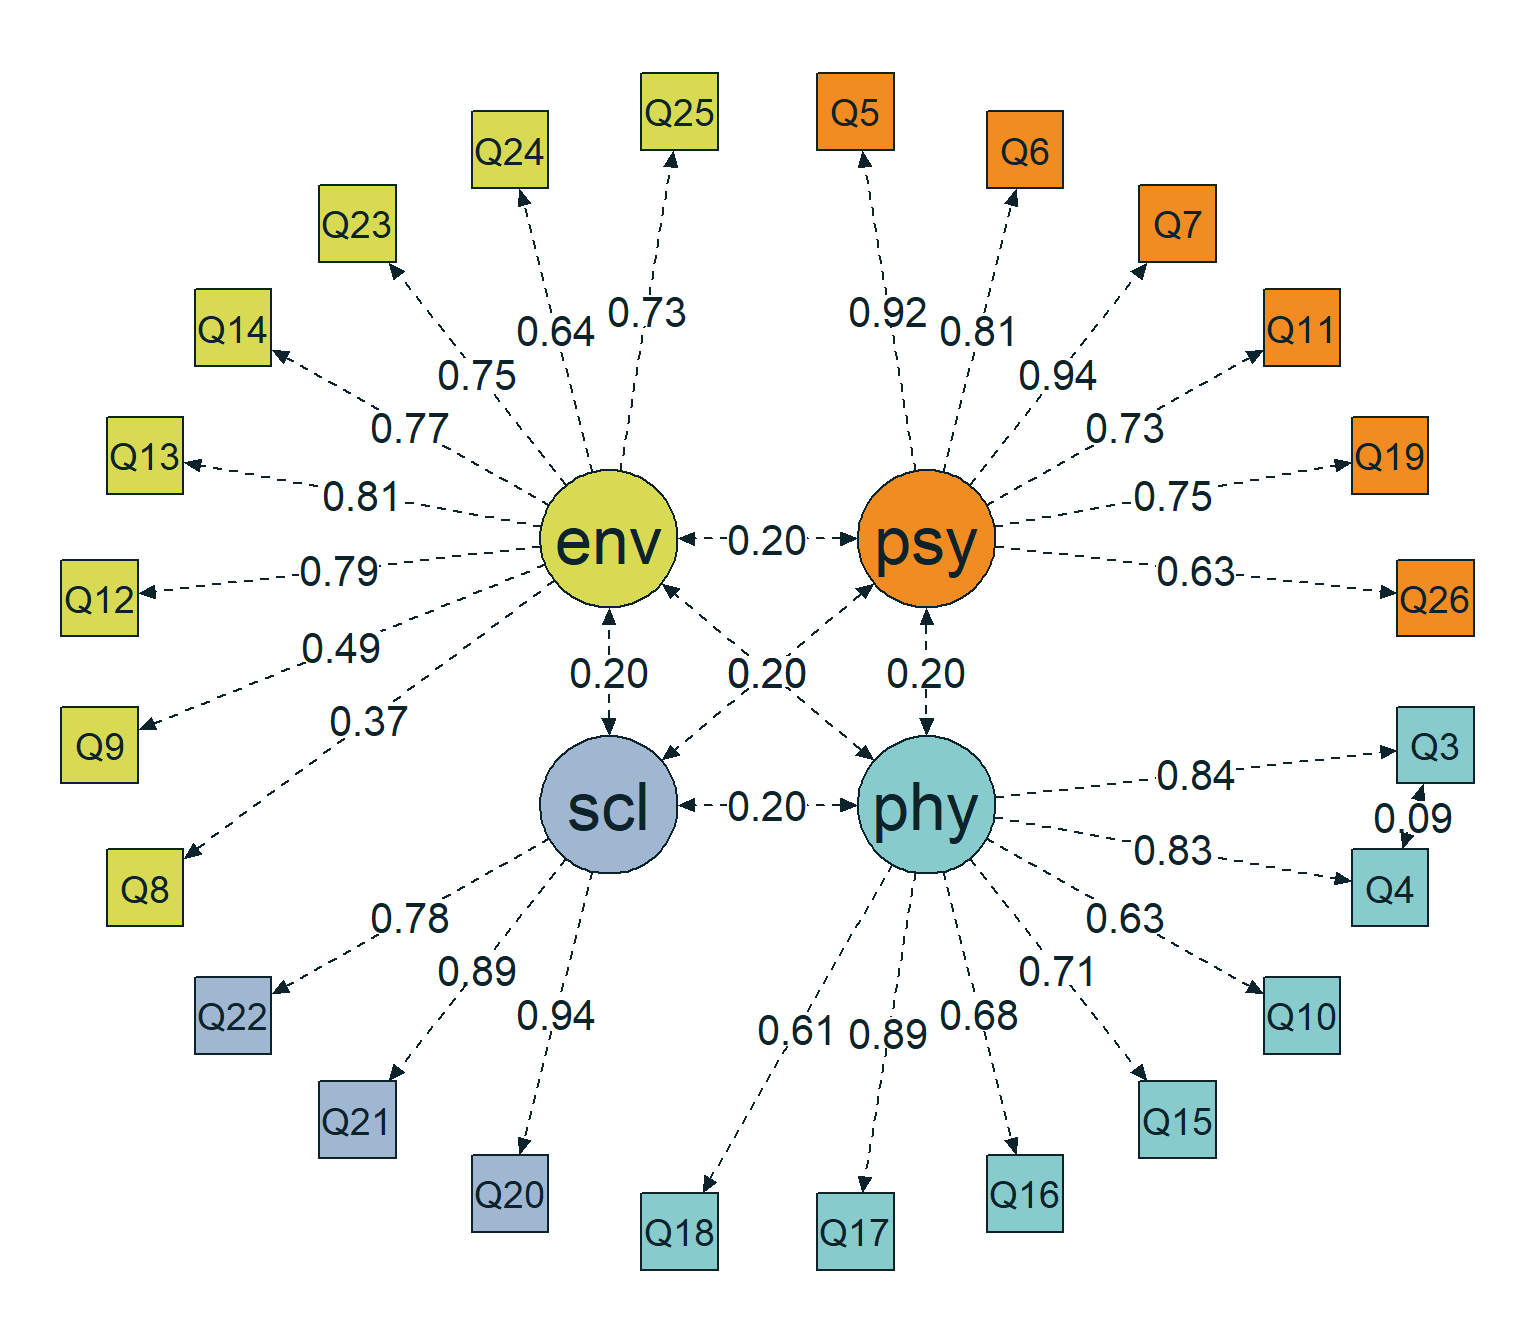
\includegraphics[keepaspectratio]{index_files/figure-latex/Scripts-AnalysisScripts-01_population_models-fig-diagram-popmodel-output-1.png}}

}

\caption{\label{fig-diagram-popmodel}Path diagram of the popmodel}

\end{figure}%

\textsubscript{Source:
\href{https://phdpablo.github.io/cfa-power/Scripts/AnalysisScripts/01_population_models-preview.html\#cell-fig-diagram-popmodel}{Population
Models}}

\subsection{Naive model}\label{naive-model}

The naive model provides an empirically grounded pessimistic scenario.
Factor loadings are derived via the Spearman-Brown prediction formula
from the lowest Cronbach's \(\alpha\) values identified in the
literature ({Mosqueira Taipe et al.}, 2026), yielding conservative
parameter estimates that push sample size requirements upward:

\begin{itemize}
\tightlist
\item
  \textbf{Approach}: Assuming equal loadings within each domain,
  \(\lambda = \sqrt{\alpha / (k - \alpha(k-1))}\) and
  \(\theta = 1 - \lambda^2\).
\item
  \textbf{Alpha sources}: Lowest domain alphas from a single study
  identified in the systematic review by {Mosqueira Taipe et al.} (2026)
  (Physical \(\alpha = 0.672\); Psychological \(\alpha = 0.704\); Social
  \(\alpha = 0.630\); Environmental \(\alpha = 0.709\)), all within the
  \(M - 1SD\) range reported by Lin \& Yao (2022).
\item
  \textbf{Interfactor correlations (\(\phi\))}: Fixed at \(0.30\) (the
  upper bound from Lin \& Yao (2022)), making factors harder to
  distinguish and yielding a deliberately conservative power estimate.
\item
  \textbf{Derived parameters}: Physical (\(\lambda = 0.4758\),
  \(\theta = 0.7736\)); Psychological (\(\lambda = 0.5328\),
  \(\theta = 0.7161\)); Social (\(\lambda = 0.6017\),
  \(\theta = 0.6379\)); Environmental (\(\lambda = 0.4832\),
  \(\theta = 0.7665\)). The residual covariance between \(Q3\) and
  \(Q4\) is adjusted to \(0.2321\).
\end{itemize}

\begin{figure}[H]

\centering{

\pandocbounded{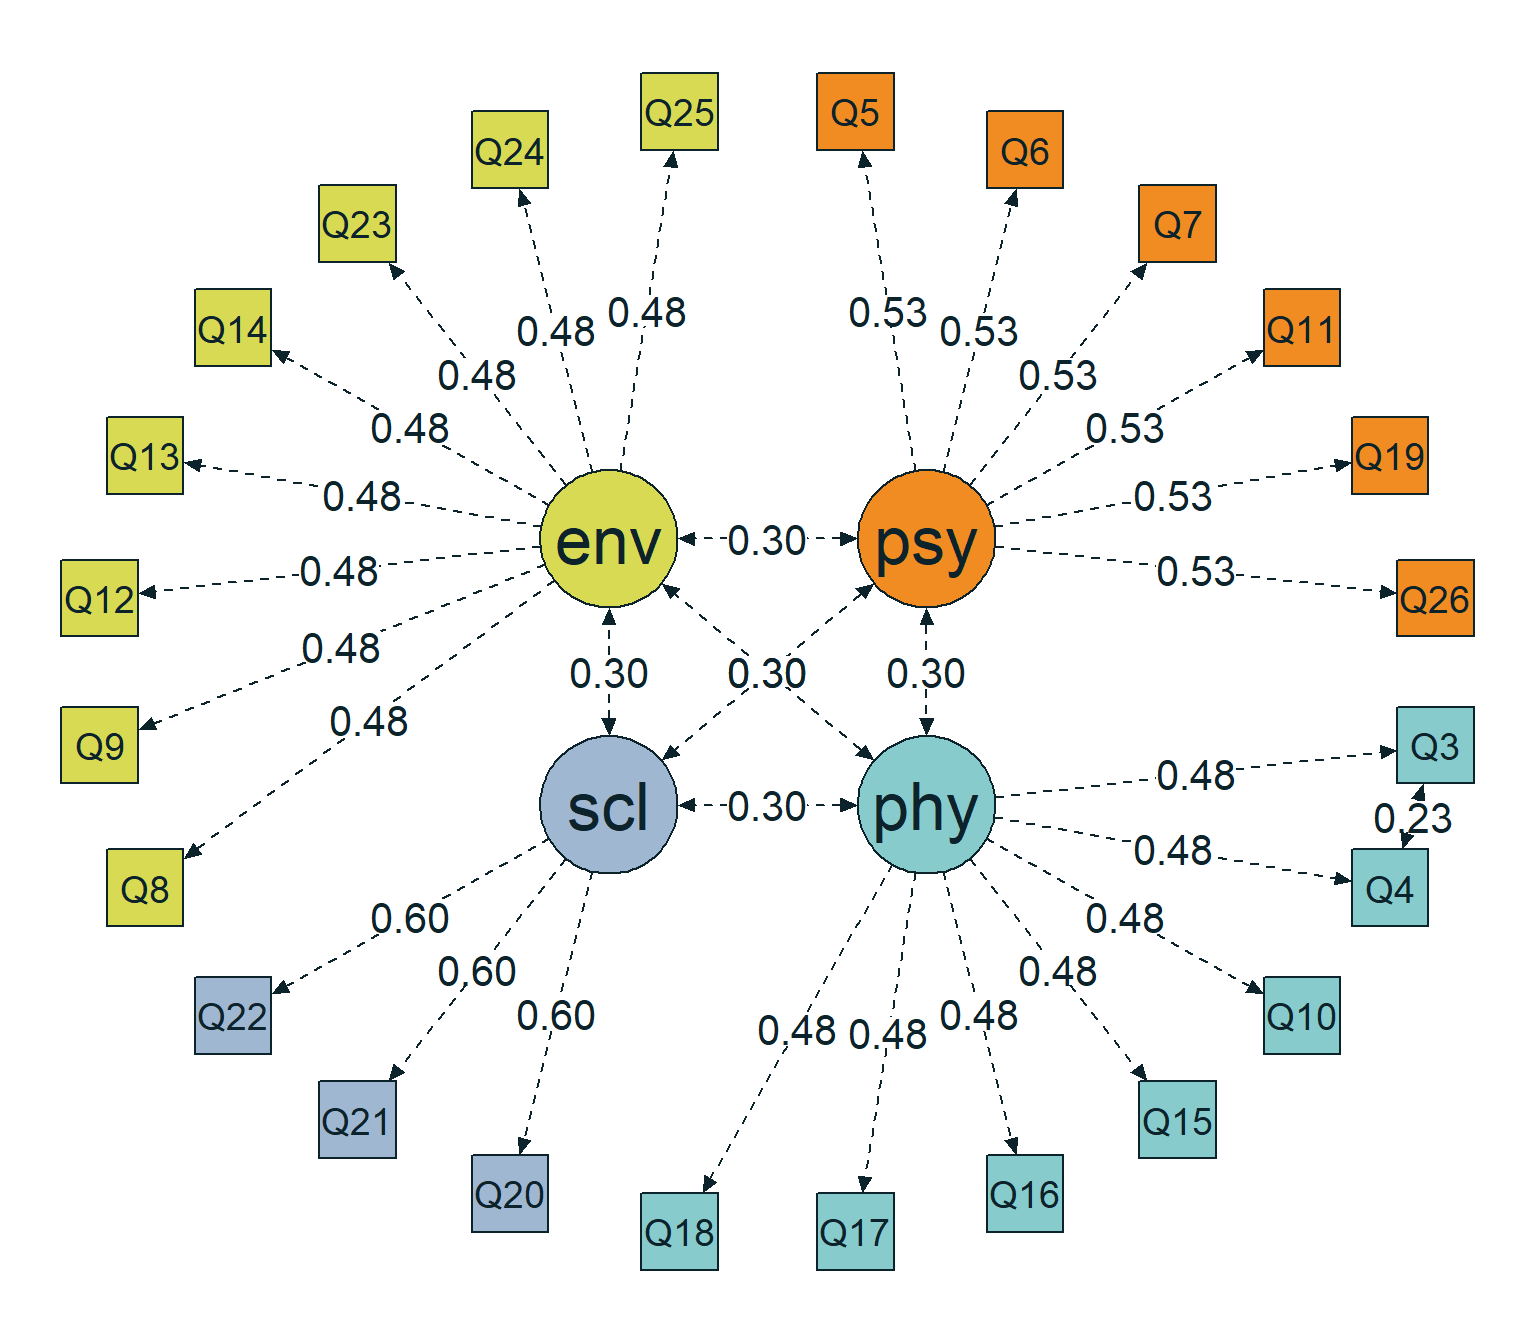
\includegraphics[keepaspectratio]{index_files/figure-latex/Scripts-AnalysisScripts-01_population_models-fig-diagram-naivemodel-output-1.png}}

}

\caption{\label{fig-diagram-naivemodel}Path diagram of the naivemodel}

\end{figure}%

\textsubscript{Source:
\href{https://phdpablo.github.io/cfa-power/Scripts/AnalysisScripts/01_population_models-preview.html\#cell-fig-diagram-naivemodel}{Population
Models}}

\subsection{Optimistic model}\label{optimistic-model}

The optimistic model applies the same Spearman-Brown derivation but
draws on the highest observed Cronbach's \(\alpha\) values per domain,
producing stronger loadings and lower residual variances relative to the
naive model ({Mosqueira Taipe et al.}, 2026):

\begin{itemize}
\tightlist
\item
  \textbf{Alpha sources}: Maximum domain alphas from the literature
  ({Mosqueira Taipe et al.}, 2026) (Physical \(\alpha = 0.860\);
  Psychological \(\alpha = 0.860\); Social \(\alpha = 0.810\);
  Environmental \(\alpha = 0.849\)), all confirmed within the
  \(M + 1SD\) range from Lin \& Yao (2022).
\item
  \textbf{Interfactor correlations (\(\phi\))}: Fixed at \(0.08\) (the
  lower bound from Lin \& Yao (2022)), so that factors are well
  distinguished and sample size requirements are reduced.
\item
  \textbf{Derived parameters}: Physical (\(\lambda = 0.6837\),
  \(\theta = 0.5326\)); Psychological (\(\lambda = 0.7113\),
  \(\theta = 0.4941\)); Social (\(\lambda = 0.7661\),
  \(\theta = 0.4130\)); Environmental (\(\lambda = 0.6424\),
  \(\theta = 0.5873\)). The residual covariance between \(Q3\) and
  \(Q4\) is adjusted to \(0.1598\).
\end{itemize}

\begin{figure}[H]

\centering{

\pandocbounded{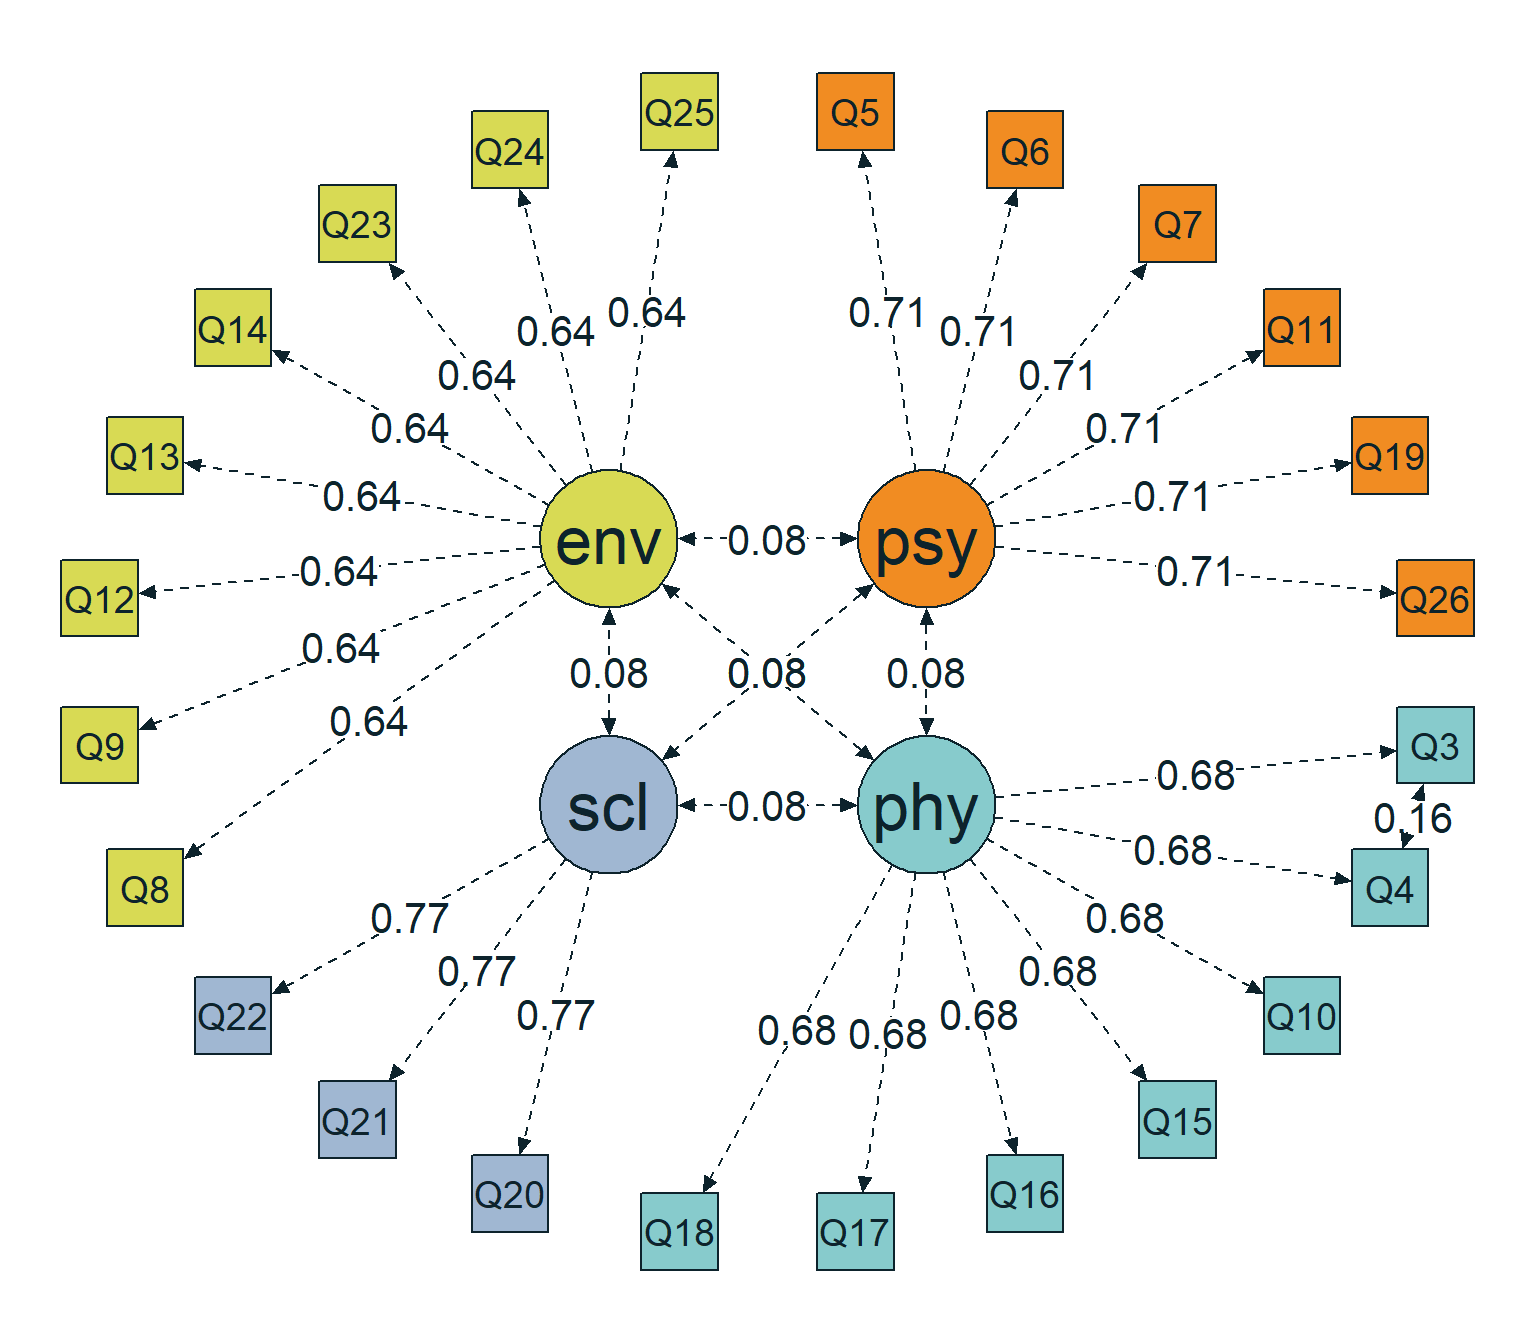
\includegraphics[keepaspectratio]{index_files/figure-latex/Scripts-AnalysisScripts-01_population_models-fig-diagram-optmodel-output-1.png}}

}

\caption{\label{fig-diagram-optmodel}Path diagram of the optmodel}

\end{figure}%

\textsubscript{Source:
\href{https://phdpablo.github.io/cfa-power/Scripts/AnalysisScripts/01_population_models-preview.html\#cell-fig-diagram-optmodel}{Population
Models}}

\subsection{Misspecification model}\label{misspecification-model}

This model defines the alternative hypothesis (\(H_1\)): a cross-loading
variant of the four-factor structure in which three empirically
motivated cross-loadings are added based on the meta-EFA results of Lin
\& Yao (2022) and the systematic review evidence in {Mosqueira Taipe et
al.} (2026):

\begin{itemize}
\tightlist
\item
  \textbf{Cross-loading 1}: Item \(Q8\) on the Psychological factor
  (\(\lambda = 0.55\)). This item showed the highest betweenness
  centrality (\(40.50\)) and was assigned to the Psychological factor in
  9 of 16 studies (Lin \& Yao, 2022).
\item
  \textbf{Cross-loading 2}: Item \(Q9\) on the Psychological factor
  (\(\lambda = 0.21\)), identified as a secondary loading in the
  five-factor EFA solution.
\item
  \textbf{Cross-loading 3}: Item \(Q15\) on the Environmental factor
  (\(\lambda = 0.24\)). ``Mobility'' conceptually bridges physical
  ability and environmental access, and this item showed the
  second-highest betweenness centrality (\(36.50\)) (Lin \& Yao, 2022).
\end{itemize}

Residual variances for cross-loaded items were recalculated to preserve
total item variance:
\(\theta = 1 - \lambda_{\text{primary}}^2 - \lambda_{\text{secondary}}^2 - 2\lambda_{\text{primary}}\lambda_{\text{secondary}}\phi\),
where \(\phi = 0.20\).

\begin{figure}[H]

\centering{

\pandocbounded{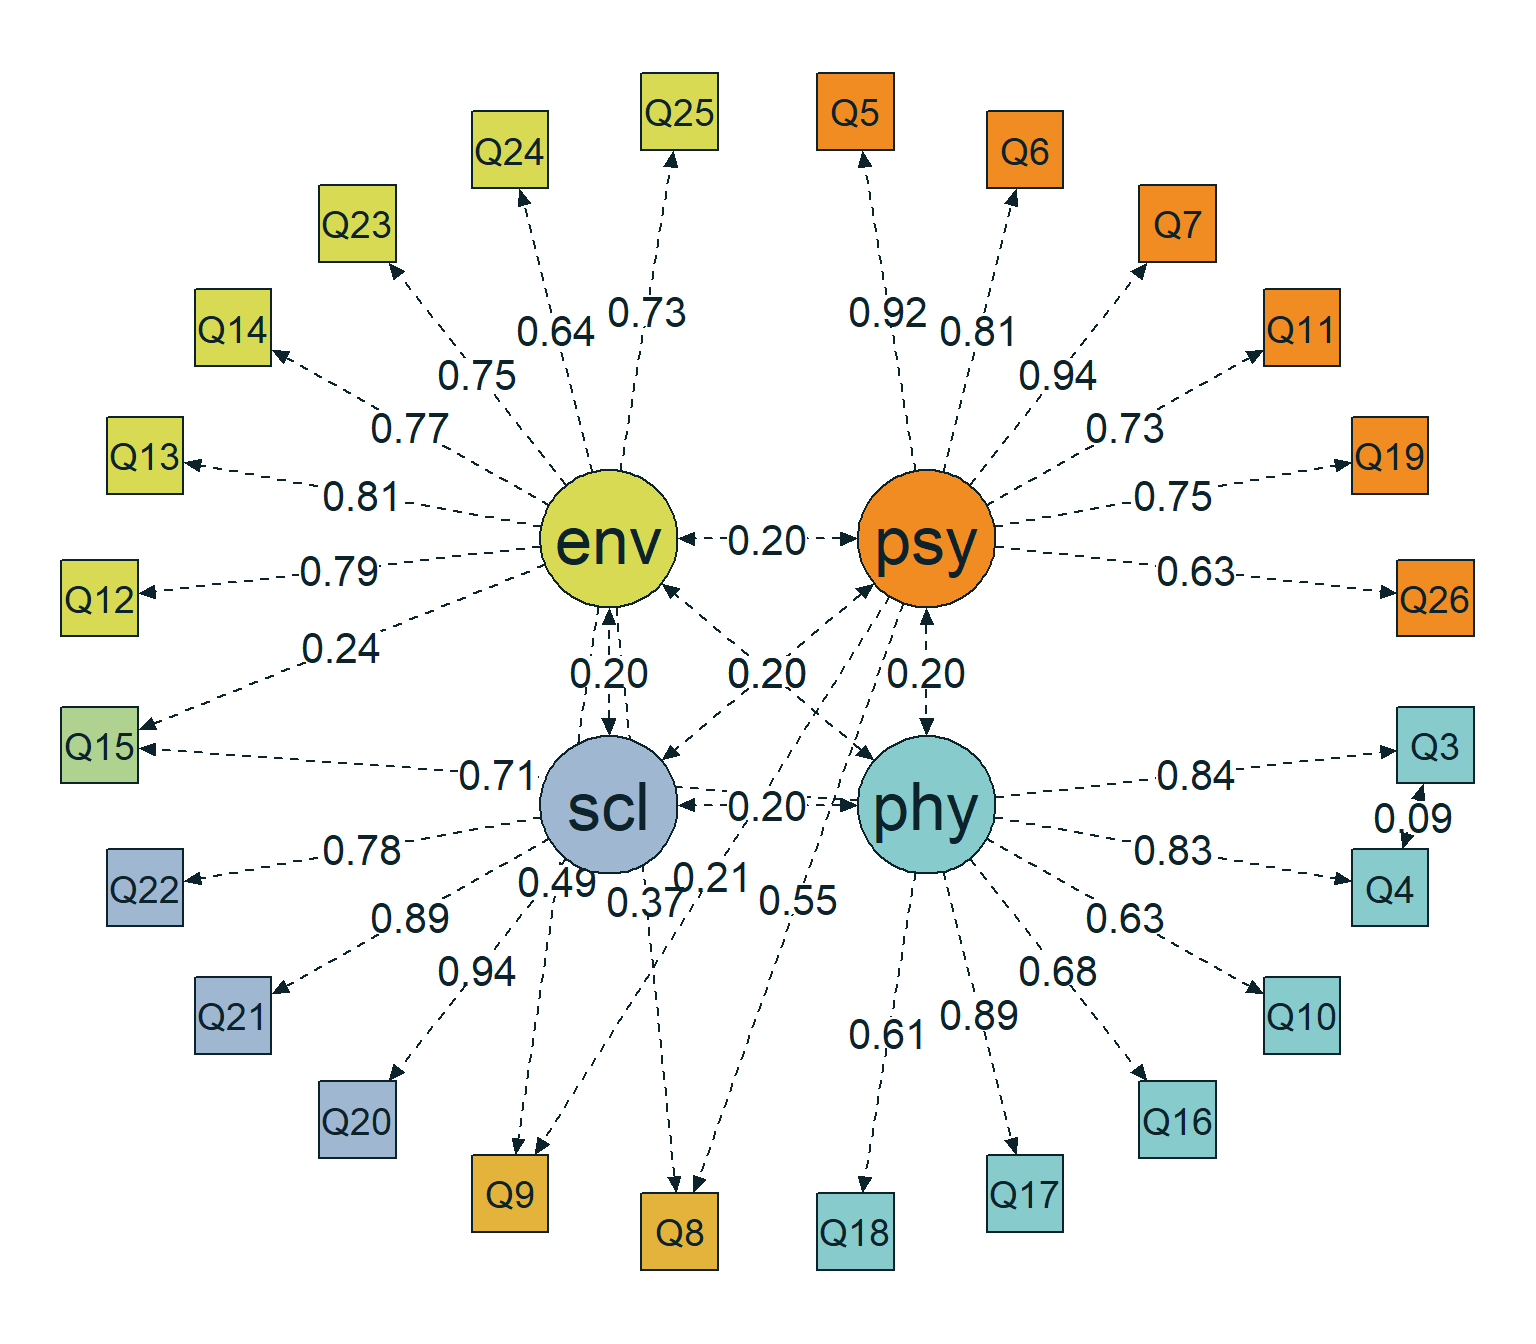
\includegraphics[keepaspectratio]{index_files/figure-latex/Scripts-AnalysisScripts-01_population_models-fig-diagram-h1model-output-1.png}}

}

\caption{\label{fig-diagram-h1model}Path diagram of the h1model}

\end{figure}%

\textsubscript{Source:
\href{https://phdpablo.github.io/cfa-power/Scripts/AnalysisScripts/01_population_models-preview.html\#cell-fig-diagram-h1model}{Population
Models}}

\subsection{Summary of population
models}\label{summary-of-population-models}

Table~\ref{tbl-pop-summary} presents all parameters of the four
population models. Table~\ref{tbl-pop-comparison} summarizes key
features across models --- minimum and maximum factor loadings, mean
loading, modal interfactor correlation, minimum and maximum residual
variances, and the residual correlation between \(Q3\) and \(Q4\) --- to
facilitate direct comparison.

{

\begin{longtable}[]{@{}
  >{\raggedright\arraybackslash}p{(\linewidth - 8\tabcolsep) * \real{0.3766}}
  >{\centering\arraybackslash}p{(\linewidth - 8\tabcolsep) * \real{0.1429}}
  >{\centering\arraybackslash}p{(\linewidth - 8\tabcolsep) * \real{0.1688}}
  >{\centering\arraybackslash}p{(\linewidth - 8\tabcolsep) * \real{0.1429}}
  >{\centering\arraybackslash}p{(\linewidth - 8\tabcolsep) * \real{0.1429}}@{}}

\caption{\label{tbl-pop-summary}Summary of population models used for
sensitivity analysis}

\tabularnewline

\toprule\noalign{}
\begin{minipage}[b]{\linewidth}\raggedright
parameters
\end{minipage} & \begin{minipage}[b]{\linewidth}\centering
popmodel
\end{minipage} & \begin{minipage}[b]{\linewidth}\centering
naivemodel
\end{minipage} & \begin{minipage}[b]{\linewidth}\centering
optmodel
\end{minipage} & \begin{minipage}[b]{\linewidth}\centering
h1model
\end{minipage} \\
\midrule\noalign{}
\endhead
\bottomrule\noalign{}
\endlastfoot
psycho=\textasciitilde Q5 & 0.9200 & 0.5328 & 0.7113 & 0.9200 \\
psycho=\textasciitilde Q6 & 0.8100 & 0.5328 & 0.7113 & 0.8100 \\
psycho=\textasciitilde Q7 & 0.9400 & 0.5328 & 0.7113 & 0.9400 \\
psycho=\textasciitilde Q11 & 0.7300 & 0.5328 & 0.7113 & 0.7300 \\
psycho=\textasciitilde Q19 & 0.7500 & 0.5328 & 0.7113 & 0.7500 \\
psycho=\textasciitilde Q26 & 0.6300 & 0.5328 & 0.7113 & 0.6300 \\
physical=\textasciitilde Q3 & 0.8400 & 0.4758 & 0.6837 & 0.8400 \\
physical=\textasciitilde Q4 & 0.8300 & 0.4758 & 0.6837 & 0.8300 \\
physical=\textasciitilde Q10 & 0.6300 & 0.4758 & 0.6837 & 0.6300 \\
physical=\textasciitilde Q15 & 0.7100 & 0.4758 & 0.6837 & 0.7100 \\
physical=\textasciitilde Q16 & 0.6800 & 0.4758 & 0.6837 & 0.6800 \\
physical=\textasciitilde Q17 & 0.8900 & 0.4758 & 0.6837 & 0.8900 \\
physical=\textasciitilde Q18 & 0.6100 & 0.4758 & 0.6837 & 0.6100 \\
social=\textasciitilde Q20 & 0.9400 & 0.6017 & 0.7661 & 0.9400 \\
social=\textasciitilde Q21 & 0.8900 & 0.6017 & 0.7661 & 0.8900 \\
social=\textasciitilde Q22 & 0.7800 & 0.6017 & 0.7661 & 0.7800 \\
environment=\textasciitilde Q8 & 0.3700 & 0.4832 & 0.6424 & 0.3700 \\
environment=\textasciitilde Q9 & 0.4900 & 0.4832 & 0.6424 & 0.4900 \\
environment=\textasciitilde Q12 & 0.7900 & 0.4832 & 0.6424 & 0.7900 \\
environment=\textasciitilde Q13 & 0.8100 & 0.4832 & 0.6424 & 0.8100 \\
environment=\textasciitilde Q14 & 0.7700 & 0.4832 & 0.6424 & 0.7700 \\
environment=\textasciitilde Q23 & 0.7500 & 0.4832 & 0.6424 & 0.7500 \\
environment=\textasciitilde Q24 & 0.6400 & 0.4832 & 0.6424 & 0.6400 \\
environment=\textasciitilde Q25 & 0.7300 & 0.4832 & 0.6424 & 0.7300 \\
Q3\textasciitilde\textasciitilde Q4 & 0.0908 & 0.2321 & 0.1598 &
0.0908 \\
psycho\textasciitilde\textasciitilde psycho & 1.0000 & 1.0000 & 1.0000 &
1.0000 \\
psycho\textasciitilde\textasciitilde physical & 0.2000 & 0.3000 & 0.0800
& 0.2000 \\
psycho\textasciitilde\textasciitilde social & 0.2000 & 0.3000 & 0.0800 &
0.2000 \\
psycho\textasciitilde\textasciitilde environment & 0.2000 & 0.3000 &
0.0800 & 0.2000 \\
physical\textasciitilde\textasciitilde physical & 1.0000 & 1.0000 &
1.0000 & 1.0000 \\
physical\textasciitilde\textasciitilde social & 0.2000 & 0.3000 & 0.0800
& 0.2000 \\
physical\textasciitilde\textasciitilde environment & 0.2000 & 0.3000 &
0.0800 & 0.2000 \\
social\textasciitilde\textasciitilde social & 1.0000 & 1.0000 & 1.0000 &
1.0000 \\
social\textasciitilde\textasciitilde environment & 0.2000 & 0.3000 &
0.0800 & 0.2000 \\
environment\textasciitilde\textasciitilde environment & 1.0000 & 1.0000
& 1.0000 & 1.0000 \\
Q5\textasciitilde\textasciitilde Q5 & 0.1536 & 0.7161 & 0.4941 &
0.1536 \\
Q6\textasciitilde\textasciitilde Q6 & 0.3439 & 0.7161 & 0.4941 &
0.3439 \\
Q7\textasciitilde\textasciitilde Q7 & 0.1164 & 0.7161 & 0.4941 &
0.1164 \\
Q11\textasciitilde\textasciitilde Q11 & 0.4671 & 0.7161 & 0.4941 &
0.4671 \\
Q19\textasciitilde\textasciitilde Q19 & 0.4375 & 0.7161 & 0.4941 &
0.4375 \\
Q26\textasciitilde\textasciitilde Q26 & 0.6031 & 0.7161 & 0.4941 &
0.6031 \\
Q3\textasciitilde\textasciitilde Q3 & 0.2944 & 0.7736 & 0.5326 &
0.2944 \\
Q4\textasciitilde\textasciitilde Q4 & 0.3111 & 0.7736 & 0.5326 &
0.3111 \\
Q10\textasciitilde\textasciitilde Q10 & 0.6031 & 0.7736 & 0.5326 &
0.6031 \\
Q15\textasciitilde\textasciitilde Q15 & 0.4959 & 0.7736 & 0.5326 &
0.3701 \\
Q16\textasciitilde\textasciitilde Q16 & 0.5376 & 0.7736 & 0.5326 &
0.5376 \\
Q17\textasciitilde\textasciitilde Q17 & 0.2079 & 0.7736 & 0.5326 &
0.2079 \\
Q18\textasciitilde\textasciitilde Q18 & 0.6279 & 0.7736 & 0.5326 &
0.6279 \\
Q20\textasciitilde\textasciitilde Q20 & 0.1164 & 0.6379 & 0.4130 &
0.1164 \\
Q21\textasciitilde\textasciitilde Q21 & 0.2079 & 0.6379 & 0.4130 &
0.2079 \\
Q22\textasciitilde\textasciitilde Q22 & 0.3916 & 0.6379 & 0.4130 &
0.3916 \\
Q8\textasciitilde\textasciitilde Q8 & 0.8631 & 0.7665 & 0.5873 &
0.4792 \\
Q9\textasciitilde\textasciitilde Q9 & 0.7599 & 0.7665 & 0.5873 &
0.6746 \\
Q12\textasciitilde\textasciitilde Q12 & 0.3759 & 0.7665 & 0.5873 &
0.3759 \\
Q13\textasciitilde\textasciitilde Q13 & 0.3439 & 0.7665 & 0.5873 &
0.3439 \\
Q14\textasciitilde\textasciitilde Q14 & 0.4071 & 0.7665 & 0.5873 &
0.4071 \\
Q23\textasciitilde\textasciitilde Q23 & 0.4375 & 0.7665 & 0.5873 &
0.4375 \\
Q24\textasciitilde\textasciitilde Q24 & 0.5904 & 0.7665 & 0.5873 &
0.5904 \\
Q25\textasciitilde\textasciitilde Q25 & 0.4671 & 0.7665 & 0.5873 &
0.4671 \\
psycho=\textasciitilde Q8 & NA & NA & NA & 0.5500 \\
psycho=\textasciitilde Q9 & NA & NA & NA & 0.2100 \\
environment=\textasciitilde Q15 & NA & NA & NA & 0.2400 \\

\end{longtable}

}

\textsubscript{Source:
\href{https://phdpablo.github.io/cfa-power/Scripts/AnalysisScripts/01_population_models-preview.html\#cell-tbl-pop-summary}{Population
Models}}

{

\begin{longtable}[]{@{}
  >{\raggedright\arraybackslash}p{(\linewidth - 8\tabcolsep) * \real{0.1923}}
  >{\centering\arraybackslash}p{(\linewidth - 8\tabcolsep) * \real{0.2308}}
  >{\centering\arraybackslash}p{(\linewidth - 8\tabcolsep) * \real{0.1923}}
  >{\centering\arraybackslash}p{(\linewidth - 8\tabcolsep) * \real{0.2051}}
  >{\centering\arraybackslash}p{(\linewidth - 8\tabcolsep) * \real{0.1538}}@{}}

\caption{\label{tbl-pop-comparison}Comparison of model variants used for
sensitivity analysis}

\tabularnewline

\toprule\noalign{}
\begin{minipage}[b]{\linewidth}\raggedright
Metric
\end{minipage} & \begin{minipage}[b]{\linewidth}\centering
Meta-analytic (popmodel)
\end{minipage} & \begin{minipage}[b]{\linewidth}\centering
Naive (naivemodel)
\end{minipage} & \begin{minipage}[b]{\linewidth}\centering
Optimistic (optmodel)
\end{minipage} & \begin{minipage}[b]{\linewidth}\centering
H1 (h1model)
\end{minipage} \\
\midrule\noalign{}
\endhead
\bottomrule\noalign{}
\endlastfoot
Loading Min & 0.37 & 0.48 & 0.64 & 0.21 \\
Loading Max & 0.94 & 0.60 & 0.77 & 0.94 \\
Mean Loading & 0.75 & 0.51 & 0.69 & 0.70 \\
Factor Correlations & 0.20 & 0.30 & 0.08 & 0.20 \\
Residual Min & 0.12 & 0.64 & 0.41 & 0.12 \\
Residual Max & 0.86 & 0.77 & 0.59 & 0.67 \\
Q3--Q4 Correlation & 0.09 & 0.23 & 0.16 & 0.09 \\

\end{longtable}

}

\textsubscript{Source:
\href{https://phdpablo.github.io/cfa-power/Scripts/AnalysisScripts/01_population_models-preview.html\#cell-tbl-pop-comparison}{Population
Models}}

\subsection{Analysis model}\label{analysis-model}

The analysis model (\texttt{analyzemodel}) serves dual purposes
depending on the simulation paradigm:

\begin{itemize}
\tightlist
\item
  \textbf{Misspecification detection}: When data are generated from the
  misspecification model (\texttt{h1model}), the analysis model acts as
  the null hypothesis (\(H_0\)) by omitting the three cross-loadings.
  Power is then the probability of correctly rejecting this
  under-parameterized model.
\item
  \textbf{Parameter recovery}: When data are generated from the
  meta-analytic, naive, or optimistic population models, the same
  structure is used to estimate the four-factor model with the
  \(Q3\)--\(Q4\) residual covariance, and power reflects the ability to
  recover individual parameters.
\end{itemize}

Key specification choices:

\begin{itemize}
\tightlist
\item
  \textbf{Identification}: Factor variances fixed to \(1\) (marker-free
  scaling), allowing all first-indicator loadings to be freely
  estimated.
\item
  \textbf{Residual covariance}: The \(Q3\)--\(Q4\) covariance is freely
  estimated, which is both theoretically justified and empirically
  supported (Lin \& Yao, 2022; {Mosqueira Taipe et al.}, 2026).
\item
  \textbf{Omitted cross-loadings}: The deliberate exclusion of
  cross-loadings for \(Q8\), \(Q9\), and \(Q15\) defines the
  misspecification that this tutorial's main analysis is designed to
  detect.
\end{itemize}

\begin{figure}[H]

\centering{

\pandocbounded{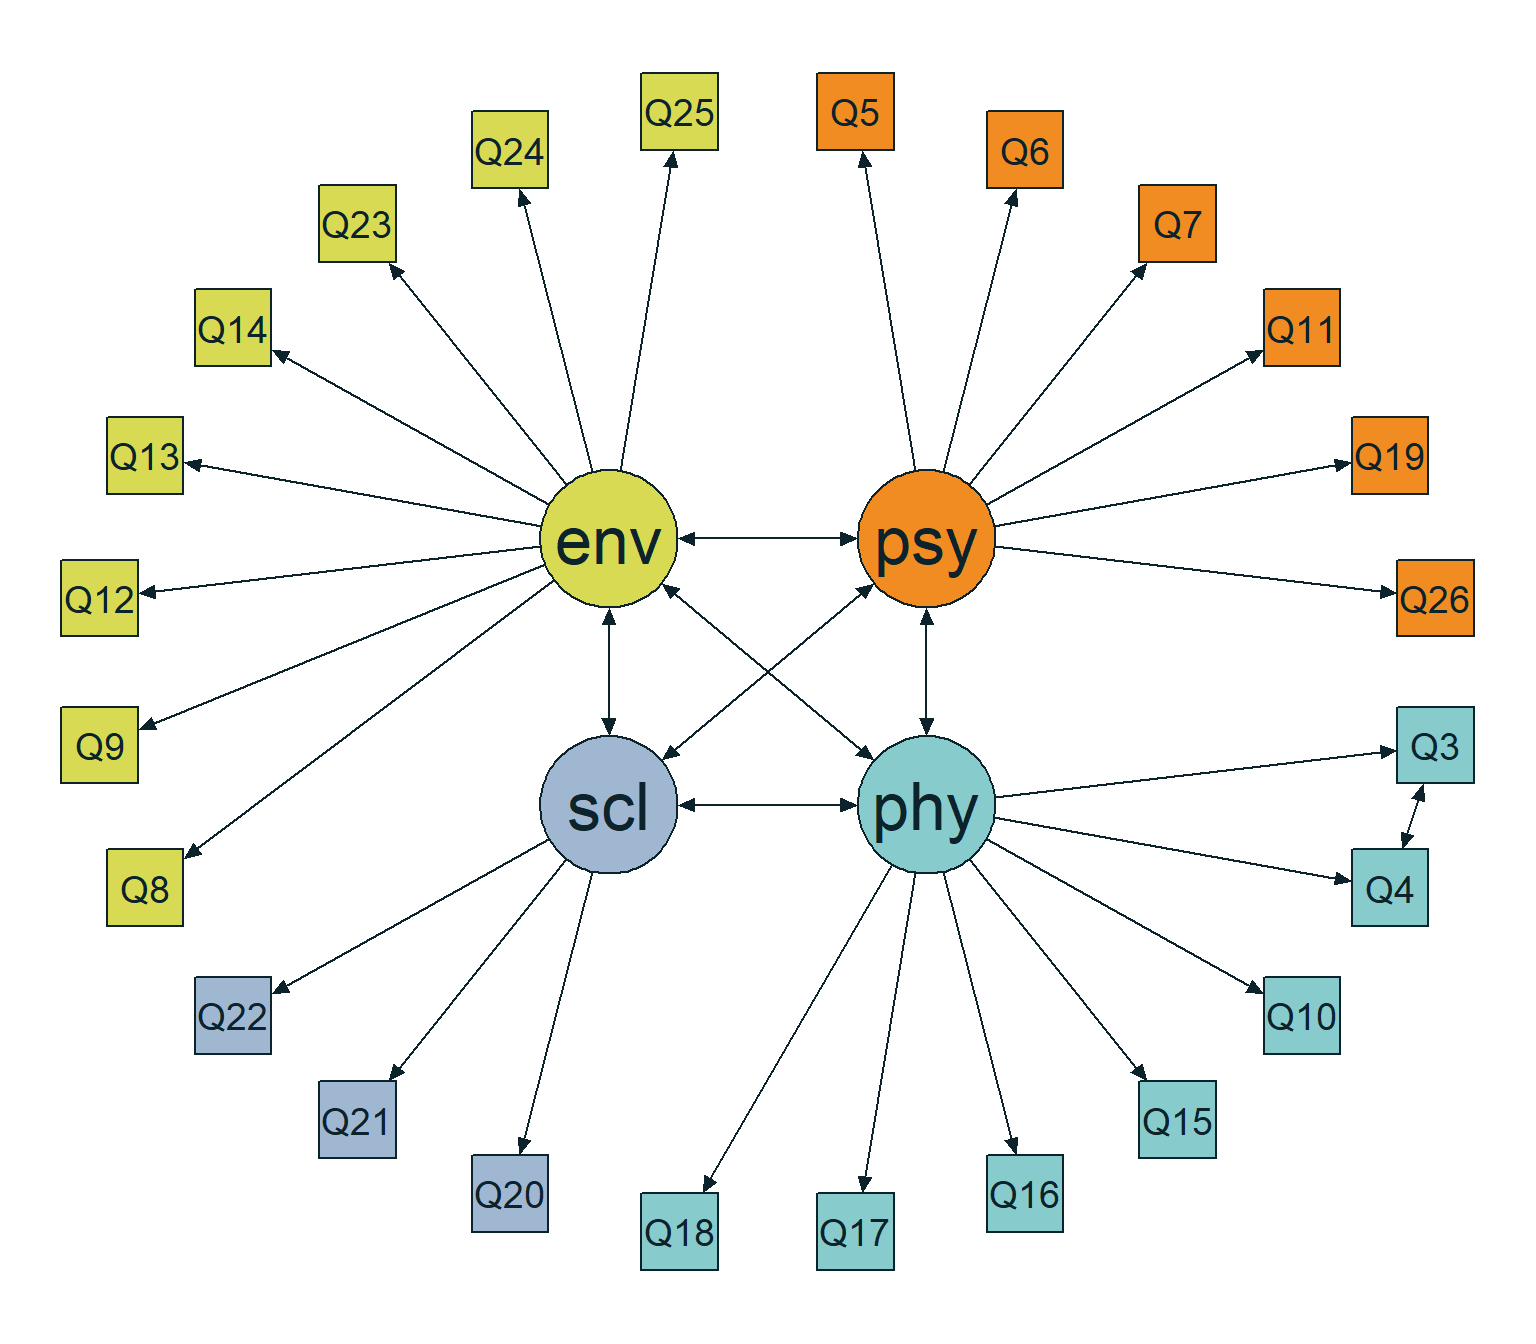
\includegraphics[keepaspectratio]{index_files/figure-latex/Scripts-AnalysisScripts-01_population_models-fig-diagram-analyzemodel-output-1.png}}

}

\caption{\label{fig-diagram-analyzemodel}Path diagram of the
analyzemodel}

\end{figure}%

\textsubscript{Source:
\href{https://phdpablo.github.io/cfa-power/Scripts/AnalysisScripts/01_population_models-preview.html\#cell-fig-diagram-analyzemodel}{Population
Models}}

\section{Analytical Power Analysis}\label{sec-analytical}

Before running any data collection, analytical power analysis answers a
fundamental planning question: how large must \(N\) be so that, if the
model is wrong by at least a specified amount, we will reject it with
acceptable probability? In SEM, the dominant analytical framework links
misspecification to the non-central \(\chi^2\) distribution through the
noncentrality parameter \(\lambda\), which scales with both \(N\) and
the magnitude of model discrepancy (Jak et al., 2021; MacCallum et al.,
1996).

\subsection{Model Degrees of Freedom}\label{sec-df}

All analytical calculations in this section depend on the model degrees
of freedom (\(df\)) --- the difference between the number of unique
variances and covariances in the observed data and the number of freely
estimated parameters. This quantity enters the non-central \(\chi^2\)
distribution directly and is therefore required before any a priori or
post hoc power calculation can proceed (Jak et al., 2021; Moshagen \&
Bader, 2024). For the hypothesized four-factor WHOQOL-BREF CFA model
analyzed here (comprising 24 observed indicators, yielding
\(p(p + 1)/2 = 300\) non-redundant sample moments and 55 freely
estimated parameters under standardized latent variables), this yields
\(df = 245\).

\subsection{A Priori: How Many Observations?}\label{sec-apriori}

\subsubsection{Model-free approach
(RMSEA-based)}\label{model-free-approach-rmsea-based}

The simplest analytical strategy sets the target effect through the
RMSEA, a noncentrality-based index that expresses misfit per degree of
freedom and is therefore comparable across models of different
complexity (MacCallum et al., 1996). Because RMSEA is directly linked to
the population minimum of the fitting function through
\(F_0 = \text{RMSEA}^2 \times df\), specifying a target RMSEA is
sufficient to define the entire noncentrality-based framework needed for
the power calculation. The approach is ``model-free'' in the sense that
no explicit population model needs to be specified: the required sample
size depends only on \(\text{RMSEA}\), \(\alpha\), desired power, and
\(df\) (Jak et al., 2021; Jobst et al., 2023).

This strategy is most appropriate when the objective is to plan sample
size for detecting overall model misspecification in a global chi-square
test of fit, rather than for testing an individual parameter restriction
(Moshagen \& Bader, 2024; Wang, 2023).

{

\begin{longtable}[]{@{}
  >{\raggedright\arraybackslash}p{(\linewidth - 4\tabcolsep) * \real{0.5195}}
  >{\centering\arraybackslash}p{(\linewidth - 4\tabcolsep) * \real{0.3247}}
  >{\raggedleft\arraybackslash}p{(\linewidth - 4\tabcolsep) * \real{0.1299}}@{}}

\caption{\label{tbl-apriori-rmsea}Analytical a priori power parameters
for RMSEA = 0.05}

\tabularnewline

\toprule\noalign{}
\begin{minipage}[b]{\linewidth}\raggedright
Metric
\end{minipage} & \begin{minipage}[b]{\linewidth}\centering
Symbol
\end{minipage} & \begin{minipage}[b]{\linewidth}\raggedleft
Value
\end{minipage} \\
\midrule\noalign{}
\endhead
\bottomrule\noalign{}
\endlastfoot
Population discrepancy & \(F_0\) & 0.613 \\
Root mean square error of approximation & \(\text{RMSEA}\) & 0.050 \\
McDonald centrality index & \(Mc\) & 0.736 \\
Goodness-of-fit index & \(\text{GFI}\) & 0.951 \\
Adjusted goodness-of-fit index & \(\text{AGFI}\) & 0.941 \\
Degrees of freedom & \(df\) & 245 \\
Required sample size & \(N\) & 100 \\
Critical chi-square & \(\chi^2_{\text{crit}}\) & 282.511 \\
Noncentrality parameter & \(\lambda\) & 60.638 \\
Significance level (alpha) & \(\alpha\) & 0.050 \\
Type II error rate (beta) & \(\beta\) & 0.1984 \\
Statistical power & \(1 - \beta\) & 0.8016 \\

\end{longtable}

}

\textsubscript{Source:
\href{https://phdpablo.github.io/cfa-power/Scripts/AnalysisScripts/02_analytical_power-preview.html\#cell-tbl-apriori-rmsea}{Analytical
Power Analysis}}

The analytical solution reported in Table~\ref{tbl-apriori-rmsea}
indicates the minimum \(N\) required to detect misfit of
\(\text{RMSEA} = 0.05\) with power \(\approx 0.80\) at
\(\alpha = 0.05\). Note that \(0.05\) refers to the misspecification
level to be detected under the alternative hypothesis, not to a
tolerated misfit level under the null (Jak et al., 2021; MacCallum et
al., 1996).

The table presents several equivalent representations of the same target
effect. The value \(F_0\) = 0.613 is the population minimum of the
fitting function, obtained from \(F_0 = df \cdot \text{RMSEA}^2\) = 245
\(\cdot\) \(0.05^2\). Alongside it, the summary also reports \(Mc\) =
0.736, \(GFI\) = 0.951, and \(AGFI\) = 0.941. These are not distinct
effect sizes but alternative summaries of the same degree of model
misfit, expressed in the metrics used by \texttt{semPower} (Moshagen \&
Bader, 2024).

The key conversion is:

\[
\lambda = (N - 1)F_0 = (N - 1)\,df\,\text{RMSEA}^2
\]

which translates the chosen misfit into the noncentrality parameter used
to locate the alternative \(\chi^2\) distribution (Jak et al., 2021;
MacCallum et al., 1996).

With \(df\) = 245, the a priori solution is \(N\) = 100. At that \(N\),
the noncentrality parameter is \(\lambda\) = 60.638 and the critical
value is \(\chi^2_c\) = 282.511. The implied \(\beta\) \(\approx\) 0.198
corresponds to power \(1 - \beta\) \(\approx\) 0.802, confirming that
\(N\) = 100 is the minimum sample size at which the target operating
characteristics are met (Jobst et al., 2023).

In Figure~\ref{fig-apriori-rmsea}, the solid red curve is the central
\(\chi^2\) under exact fit, the dashed blue curve is the noncentral
\(\chi^2\) under the target misspecification, and the vertical dotted
line at \(\chi^2\) = 282.511 is the decision threshold (Jak et al.,
2021; Moshagen \& Bader, 2024).

\begin{figure}[H]

\centering{

\pandocbounded{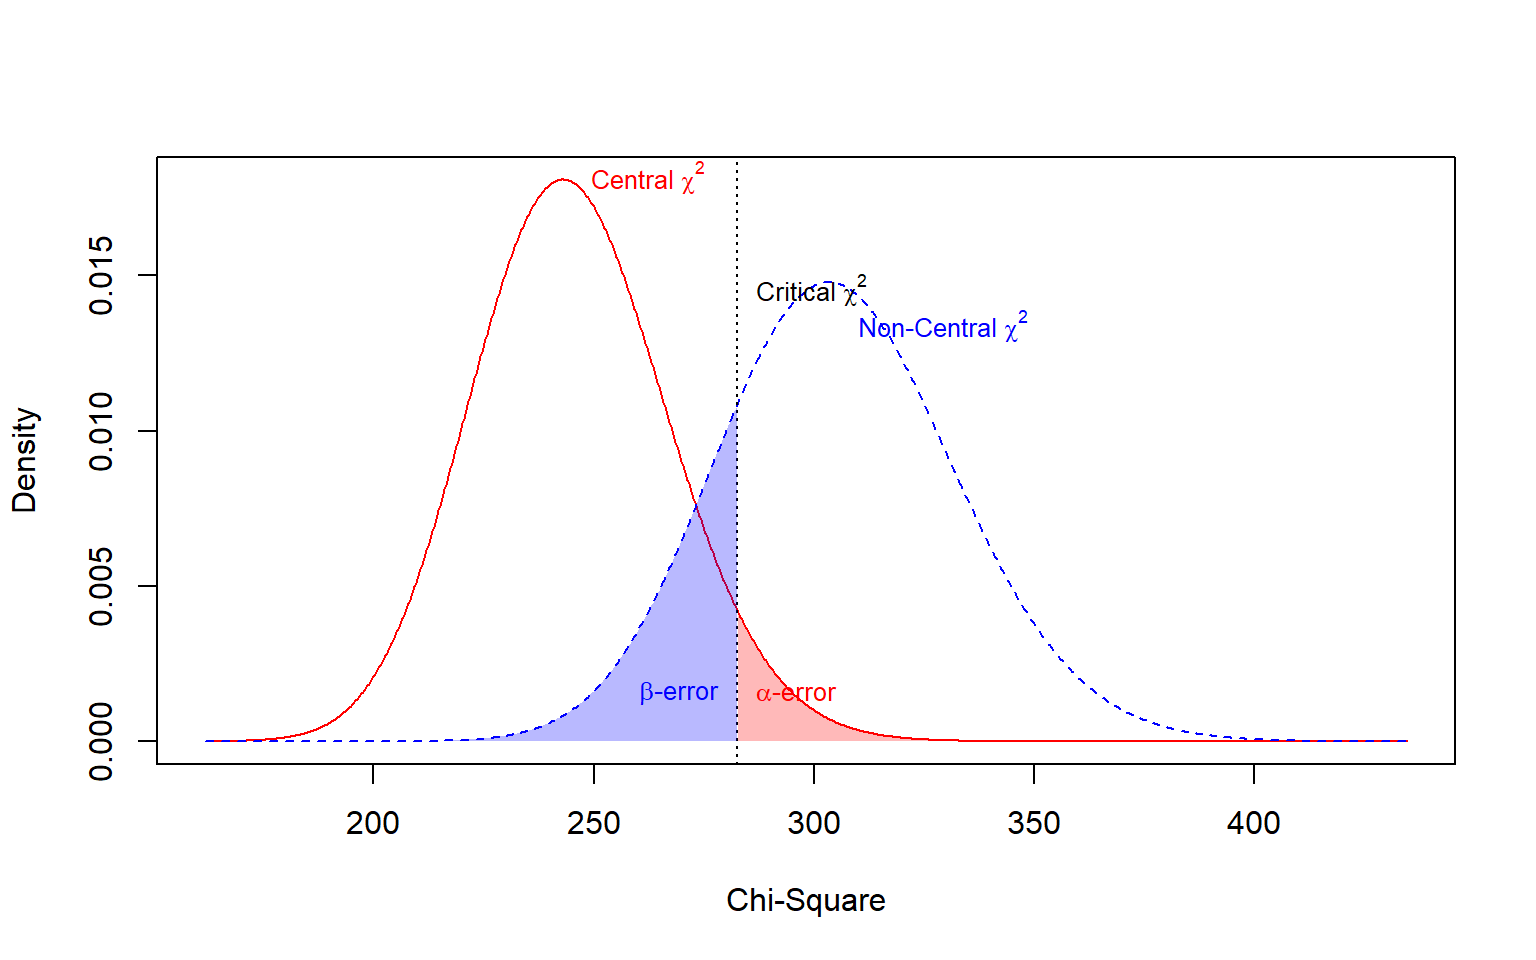
\includegraphics[keepaspectratio]{index_files/figure-latex/Scripts-AnalysisScripts-02_analytical_power-fig-apriori-rmsea-output-1.png}}

}

\caption{\label{fig-apriori-rmsea}A priori power analysis for exact fit
with RMSEA-based effect size}

\end{figure}%

\textsubscript{Source:
\href{https://phdpablo.github.io/cfa-power/Scripts/AnalysisScripts/02_analytical_power-preview.html\#cell-fig-apriori-rmsea}{Analytical
Power Analysis}}

\subsubsection{Model-based approach}\label{model-based-approach}

When substantive theory specifies the population structure, a
model-based power analysis is more informative: rather than setting
misfit to a generic RMSEA value, the effect is implied by the
discrepancy between an explicitly defined population model and the
restricted analysis model (Feng \& Hancock, 2023; Wang, 2023). This
makes the sample size estimate dependent on the hypothesized parameter
configuration rather than on a conventional threshold.

\texttt{semPower.powerLav()} implements this by fitting the null model
to the population-implied covariance matrix and translating the
resulting discrepancy into \(F_0\) and then into
\(\lambda = (N - 1)F_0\). When \texttt{modelH1} is omitted, the null
model is evaluated against the saturated model, making the analysis a
global test of fit rather than a test of any single restriction (Jobst
et al., 2023; Moshagen \& Bader, 2024). Because the effect is generated
from the full model specification, any change to loadings, factor
correlations, or residual variances will alter the required \(N\) --- an
important point when conducting sensitivity analyses (Buchberger et al.,
2024).

{

\begin{longtable}[]{@{}
  >{\raggedright\arraybackslash}p{(\linewidth - 4\tabcolsep) * \real{0.5195}}
  >{\centering\arraybackslash}p{(\linewidth - 4\tabcolsep) * \real{0.3247}}
  >{\raggedleft\arraybackslash}p{(\linewidth - 4\tabcolsep) * \real{0.1299}}@{}}

\caption{\label{tbl-apriori-popmodel}Analytical a priori power
parameters for model-based approach (h1model vs analyzemodel)}

\tabularnewline

\toprule\noalign{}
\begin{minipage}[b]{\linewidth}\raggedright
Metric
\end{minipage} & \begin{minipage}[b]{\linewidth}\centering
Symbol
\end{minipage} & \begin{minipage}[b]{\linewidth}\raggedleft
Value
\end{minipage} \\
\midrule\noalign{}
\endhead
\bottomrule\noalign{}
\endlastfoot
Population discrepancy & \(F_0\) & 0.579 \\
Root mean square error of approximation & \(\text{RMSEA}\) & 0.049 \\
McDonald centrality index & \(Mc\) & 0.749 \\
Standardized root mean square residual & \(\text{SRMR}\) & 0.067 \\
Comparative fit index & \(\text{CFI}\) & 0.960 \\
Degrees of freedom & \(df\) & 245 \\
Required sample size & \(N\) & 106 \\
Critical chi-square & \(\chi^2_{\text{crit}}\) & 282.511 \\
Noncentrality parameter & \(\lambda\) & 60.793 \\
Significance level (alpha) & \(\alpha\) & 0.050 \\
Type II error rate (beta) & \(\beta\) & 0.1968 \\
Statistical power & \(1 - \beta\) & 0.8032 \\

\end{longtable}

}

\textsubscript{Source:
\href{https://phdpablo.github.io/cfa-power/Scripts/AnalysisScripts/02_analytical_power-preview.html\#cell-tbl-apriori-popmodel}{Analytical
Power Analysis}}

The model-based analytical solution in Table~\ref{tbl-apriori-popmodel}
reports a population discrepancy of \(F_0\) = 0.579, equivalently
expressed as \(\text{RMSEA}\) = 0.049 and \(Mc\) = 0.749. With \(df\) =
245, the required sample size is \(N\) = 106, and the corresponding
critical chi-square is 282.511. The noncentrality parameter is
\(\lambda\) = 60.793, consistent with \((N - 1)F_0\) at the obtained
solution. The error rates are \(\alpha\) = 0.05, \(\beta\) = 0.197, and
power = 0.803, confirming that the design conditions are met at \(N\) =
106. The corresponding distribution curves are displayed in
Figure~\ref{fig-apriori-popmodel}:

\begin{figure}[H]

\centering{

\pandocbounded{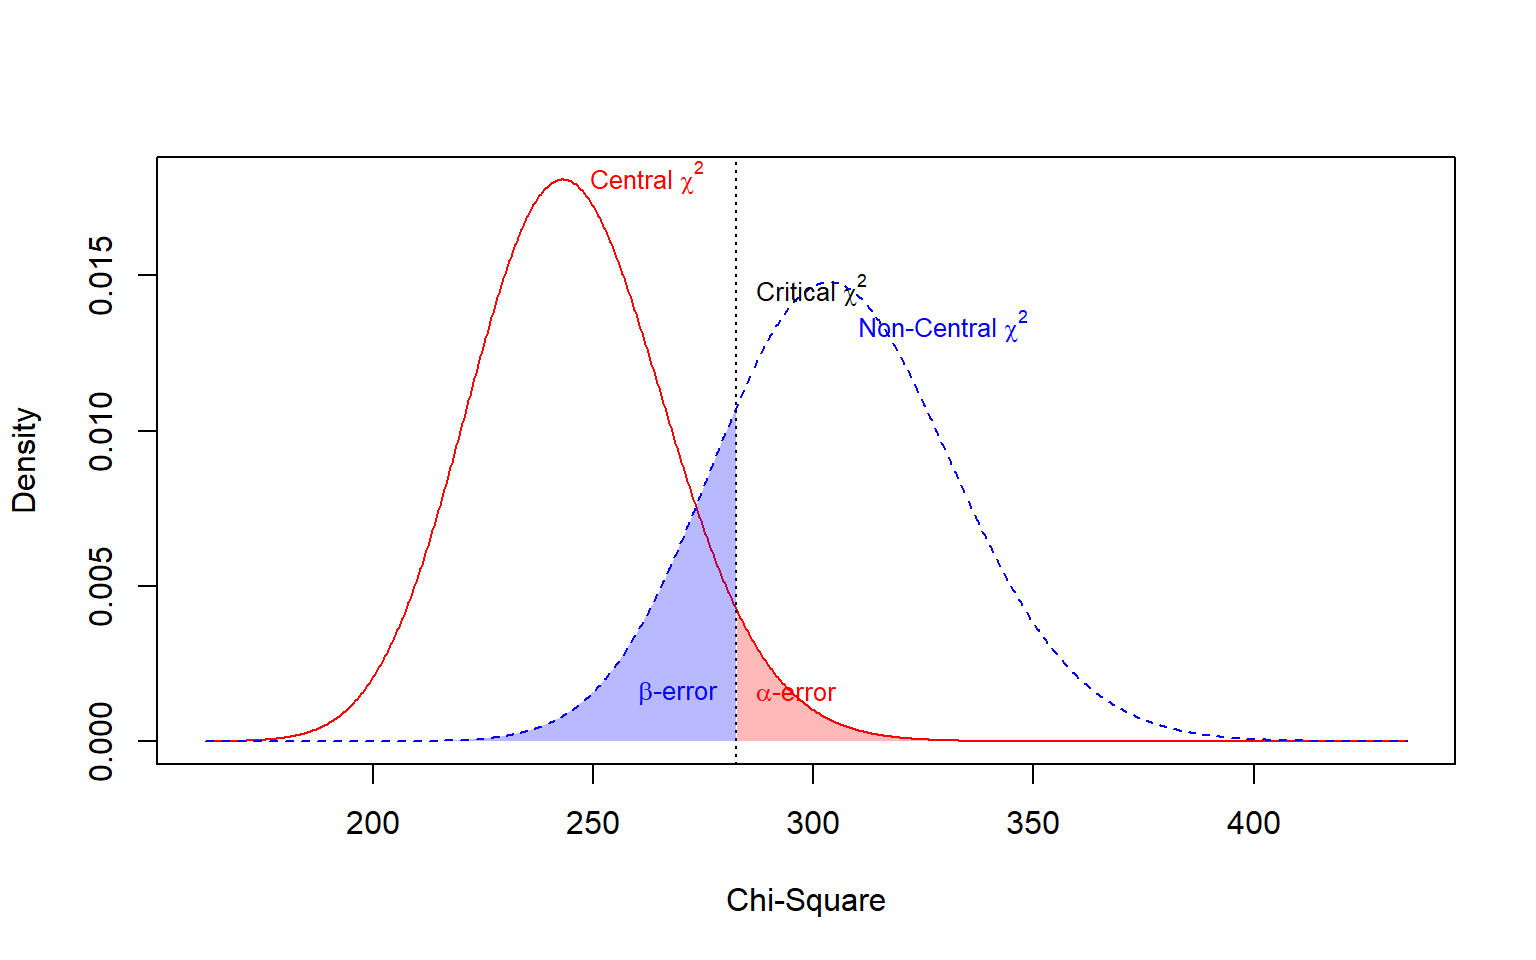
\includegraphics[keepaspectratio]{index_files/figure-latex/Scripts-AnalysisScripts-02_analytical_power-fig-apriori-popmodel-output-1.png}}

}

\caption{\label{fig-apriori-popmodel}A priori power analysis Model-based
approach (h1model vs analyzemodel)}

\end{figure}%

\textsubscript{Source:
\href{https://phdpablo.github.io/cfa-power/Scripts/AnalysisScripts/02_analytical_power-preview.html\#cell-fig-apriori-popmodel}{Analytical
Power Analysis}}

\subsection{Power Curves}\label{sec-power-curves}

Power curves visualize the relationship between sample size and the
probability of detecting a prespecified degree of model
misspecification, holding \(\alpha\) and \(df\) constant. They serve as
a planning aid by showing at a glance which \(N\) values are
underpowered and where additional observations yield diminishing returns
(Moshagen \& Bader, 2024).

\subsubsection{Model-free approach
(RMSEA-based)}\label{model-free-approach-rmsea-based-1}

In the model-free setup, the power function depends entirely on
\(\text{RMSEA}\), \(df\), and \(\alpha\) --- not on any substantive
model parameters. Representing this function graphically answers a
direct planning question: for a model with fixed \(df\), how large must
\(N\) be to achieve a sufficiently high probability of detecting misfit
of at least the target magnitude (Jak et al., 2021; Jobst et al., 2023)?
This visualization is especially useful when the research objective
concerns global fit rather than individual parameter restrictions, and
it also makes it easy to communicate design justification to reviewers
or funding agencies (Moshagen \& Bader, 2024; Wang, 2023).

\begin{figure}[H]

\centering{

\pandocbounded{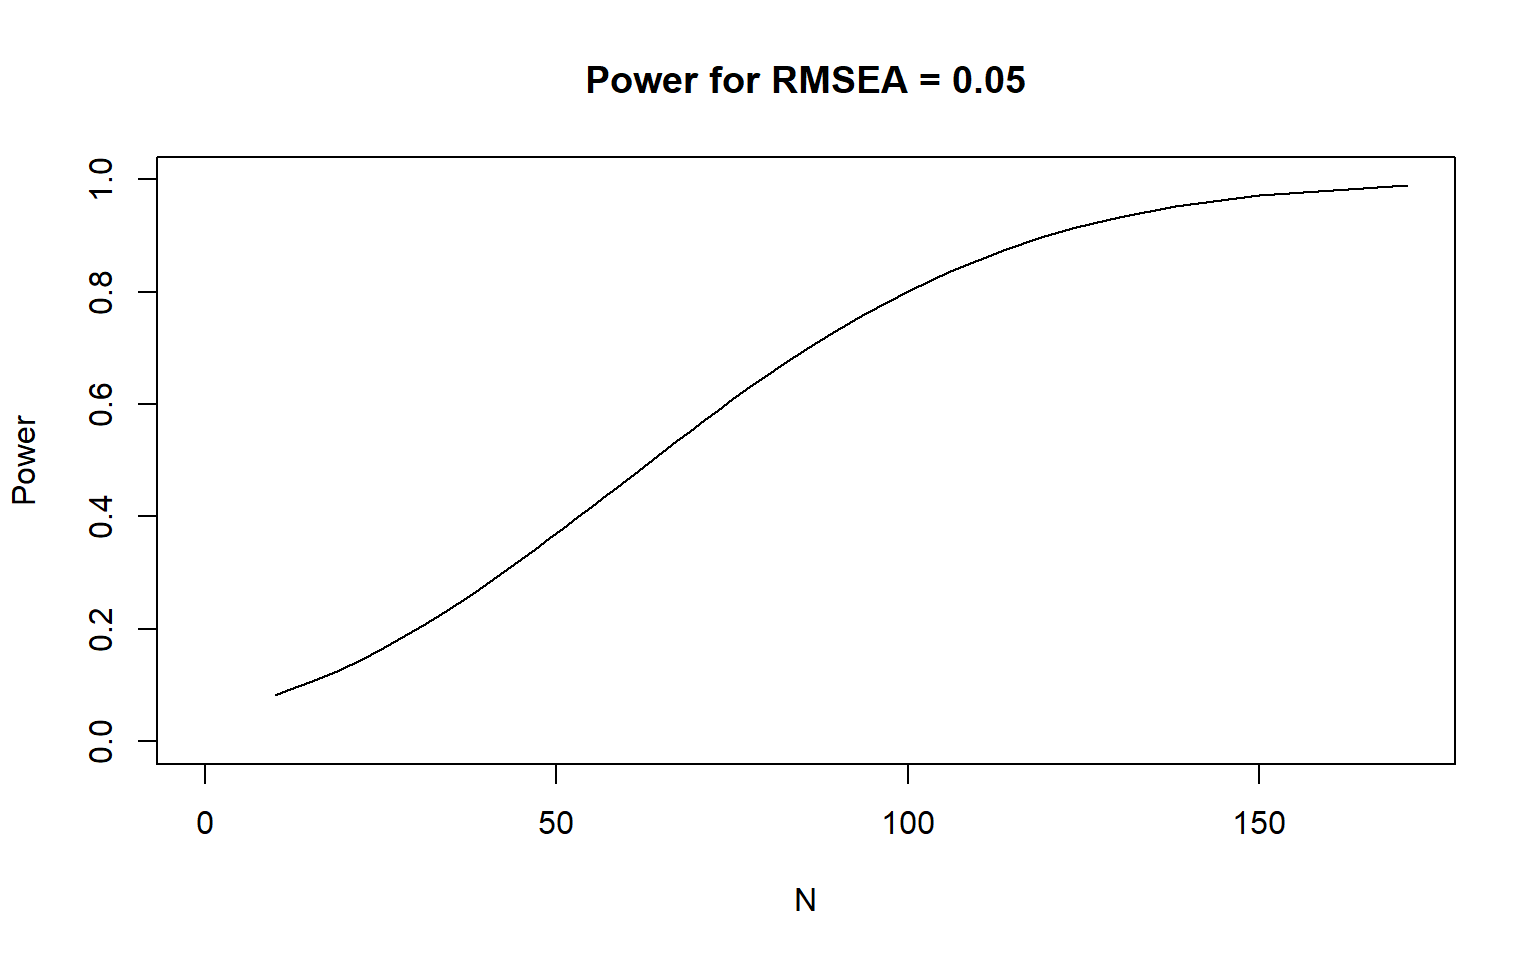
\includegraphics[keepaspectratio]{index_files/figure-latex/Scripts-AnalysisScripts-02_analytical_power-fig-power-rmsea-output-1.png}}

}

\caption{\label{fig-power-rmsea}Power as a function of sample size for
RMSEA = 0.05}

\end{figure}%

\textsubscript{Source:
\href{https://phdpablo.github.io/cfa-power/Scripts/AnalysisScripts/02_analytical_power-preview.html\#cell-fig-power-rmsea}{Analytical
Power Analysis}}

Power increases monotonically with \(N\). At the lower end of the range,
the curve is well below the target threshold, indicating insufficient
sensitivity to detect the prespecified misspecification; at higher
\(N\), it approaches the ceiling. The crossing point between the curve
and the target power level identifies the minimum adequate sample size,
and the shape of the curve shows how quickly additional observations
convert into detection probability in this particular setting.

\subsubsection{Model-based approach}\label{model-based-approach-1}

When the effect is grounded in an explicitly specified population model,
the power curve traces the same monotonic pattern but now reflects the
particular covariance structure implied by the substantive hypotheses
(Buchberger et al., 2024; Feng \& Hancock, 2023).
\texttt{semPower.powerPlot()} evaluates the previously specified
model-based effect at each \(N\) in the grid, so the curve is a
design-oriented summary of how sensitivity changes as sample size grows
--- without re-estimating any parameters (Moshagen \& Bader, 2024).

\begin{figure}[H]

\centering{

\pandocbounded{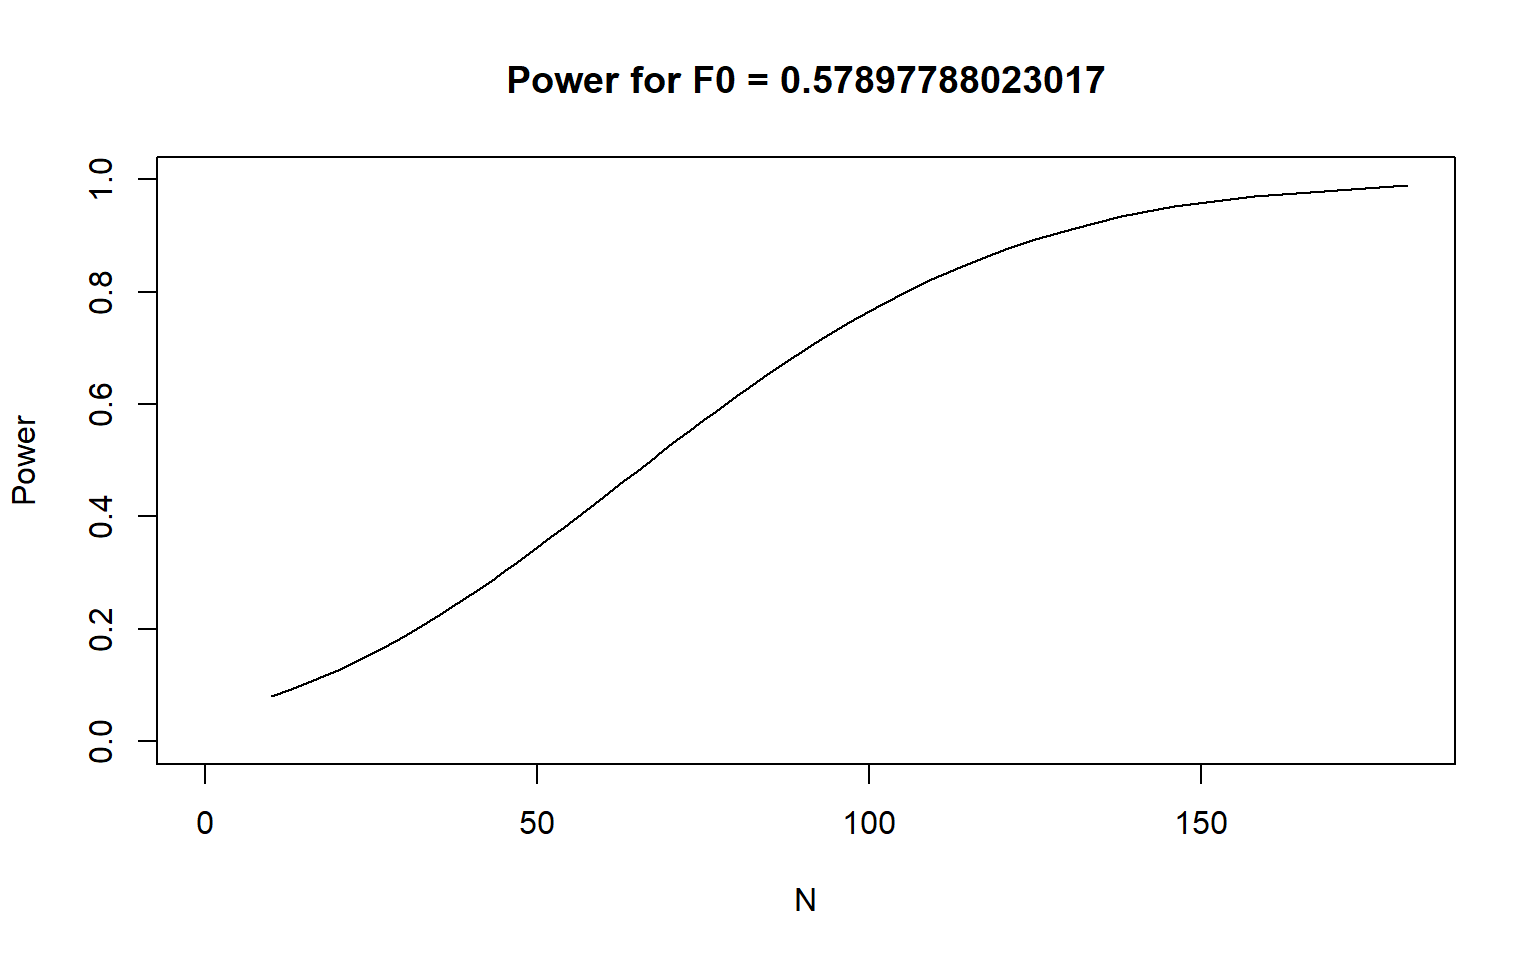
\includegraphics[keepaspectratio]{index_files/figure-latex/Scripts-AnalysisScripts-02_analytical_power-fig-power-popmodel-output-1.png}}

}

\caption{\label{fig-power-popmodel}Power as a function of sample size
for the population model (popModel)}

\end{figure}%

\textsubscript{Source:
\href{https://phdpablo.github.io/cfa-power/Scripts/AnalysisScripts/02_analytical_power-preview.html\#cell-fig-power-popmodel}{Analytical
Power Analysis}}

The plot titled Power for \(F_0\) = 0.579 shows a clear monotonic
increase. At the lower end, power hovers near \(0.07\)--\(0.10\),
indicating inadequate sensitivity for small samples. A period of rapid
growth occurs between roughly \(N = 60\) and \(N = 120\), where each
additional observation translates into a substantial gain. The
conventional \(0.80\) threshold is crossed at approximately
\(N \approx 106\), and power approaches \(0.95\) around
\(N \approx 140\), with further gains becoming marginal above that.

\subsection{Summary table}\label{summary-table}

Table~\ref{tbl-analytical-summary} compares the analytical power
solutions. The model-based global fit test requires \(N = 106\), closely
matching the model-free RMSEA-based target (\(N = 100\)). This
convergence occurs because the misspecification introduced by the three
cross-loadings translates into an implied \(\text{RMSEA} = 0.0486\),
almost identical to the generic \(0.05\) threshold.

{

\begin{longtable}[]{@{}
  >{\raggedright\arraybackslash}p{(\linewidth - 8\tabcolsep) * \real{0.4875}}
  >{\raggedright\arraybackslash}p{(\linewidth - 8\tabcolsep) * \real{0.1375}}
  >{\centering\arraybackslash}p{(\linewidth - 8\tabcolsep) * \real{0.1125}}
  >{\centering\arraybackslash}p{(\linewidth - 8\tabcolsep) * \real{0.1625}}
  >{\centering\arraybackslash}p{(\linewidth - 8\tabcolsep) * \real{0.0750}}@{}}

\caption{\label{tbl-analytical-summary}Summary of analytical power
analysis results}

\tabularnewline

\toprule\noalign{}
\begin{minipage}[b]{\linewidth}\raggedright
Method
\end{minipage} & \begin{minipage}[b]{\linewidth}\raggedright
N Required
\end{minipage} & \begin{minipage}[b]{\linewidth}\centering
Power
\end{minipage} & \begin{minipage}[b]{\linewidth}\centering
Implied RMSEA
\end{minipage} & \begin{minipage}[b]{\linewidth}\centering
df
\end{minipage} \\
\midrule\noalign{}
\endhead
\bottomrule\noalign{}
\endlastfoot
Model-free a priori (RMSEA = .05) & 100 & 0.8016 & 0.0500 & 245 \\
Model-based global fit (h1model vs.~saturated) & 106 & 0.8032 & 0.0486 &
245 \\

\end{longtable}

}

\textsubscript{Source:
\href{https://phdpablo.github.io/cfa-power/Scripts/AnalysisScripts/02_analytical_power-preview.html\#cell-tbl-analytical-summary}{Analytical
Power Analysis}}

\begin{tcolorbox}[enhanced jigsaw, arc=.35mm, bottomrule=.15mm, bottomtitle=1mm, breakable, colback=white, colbacktitle=quarto-callout-important-color!10!white, colframe=quarto-callout-important-color-frame, coltitle=black, left=2mm, leftrule=.75mm, opacityback=0, opacitybacktitle=0.6, rightrule=.15mm, title=\textcolor{quarto-callout-important-color}{\faExclamation}\hspace{0.5em}{Limitations of the Analytical Approach}, titlerule=0mm, toprule=.15mm, toptitle=1mm]

The RMSEA/\(\chi^2\)-based analytical method assumes continuous,
multivariate normal data and Maximum Likelihood estimation. It can yield
biased sample size estimates when distributions are non-normal, data are
ordinal, or missing data reduce estimation efficiency. Furthermore,
because power is framed around global misfit, the analytical approach
provides no information about whether \(N\) is sufficient to detect
specific weak loadings, factor correlations, or structural paths. These
limitations motivate the simulation-based extensions developed in
subsequent sections.

\end{tcolorbox}

\section{Monte Carlo Simulation: Ideal Conditions}\label{sec-sim-ideal}

Simulation-based power analysis in SEM operates on a different logic
from its analytical counterpart. Rather than deriving power from the
non-central \(\chi^2\) distribution, the approach repeatedly generates
data from an assumed population model, fits the analysis model to each
replicate, and summarizes rejection rates empirically. This makes the
framework far more flexible: it can accommodate complex data conditions,
evaluate multiple fit criteria simultaneously, and quantify estimation
quality --- bias, standard error accuracy, and coverage --- alongside
power (Muthén \& Muthén, 2002; Pornprasertmanit et al., 2021).

The central distinction in the design is between the
\emph{data-generating model} and the \emph{analysis model} (Feng \&
Hancock, 2023). The former defines the population from which replicated
samples are drawn; the latter defines the structure that is repeatedly
fit to each sample. Statistical power in SEM depends not only on \(N\),
but on the discrepancy between these two models, so this separation is
essential (Feng \& Hancock, 2023; Jobst et al., 2023).

In the main analysis, the reference condition uses data generated from
\texttt{popmodel}, while the alternative condition uses data generated
from \texttt{h1model} --- a structurally equivalent model with three
additional cross-loadings. The analysis model (\texttt{analyzemodel})
omits those cross-loadings, so power reflects the probability that
global fit indices flag this deliberate misspecification. Varying \(N\)
across a predefined sequence turns the simulation into a sample size
planning exercise: as \(N\) grows, the sampling distributions under the
reference and alternative conditions separate, and the probability of
correctly flagging the misspecified condition increases (Feng \&
Hancock, 2023; Jobst et al., 2023).

Power based on fit indices is therefore interpreted as the probability
that a rejection rule --- calibrated from the reference distribution at
\(\alpha\) --- classifies data generated under the alternative as
showing worse fit than expected under the well-fitting model.
Practically, this shifts the inferential focus from testing a single
parameter to evaluating whether global fit criteria are sensitive enough
to detect a substantively meaningful form of misspecification across
plausible sample sizes (Liang \& Sterba, 2024; Wang, 2023).

\subsection{Main analysis under ideal
conditions}\label{main-analysis-under-ideal-conditions}

The Figure~\ref{fig-fit-curve-ideal} and
Figure~\ref{fig-power-curve-ideal} present the main results for the
comparison between \texttt{popmodel} and \texttt{h1model} under ideal
conditions (multivariate normality, no missing data).

\begin{figure}[H]

\centering{

\pandocbounded{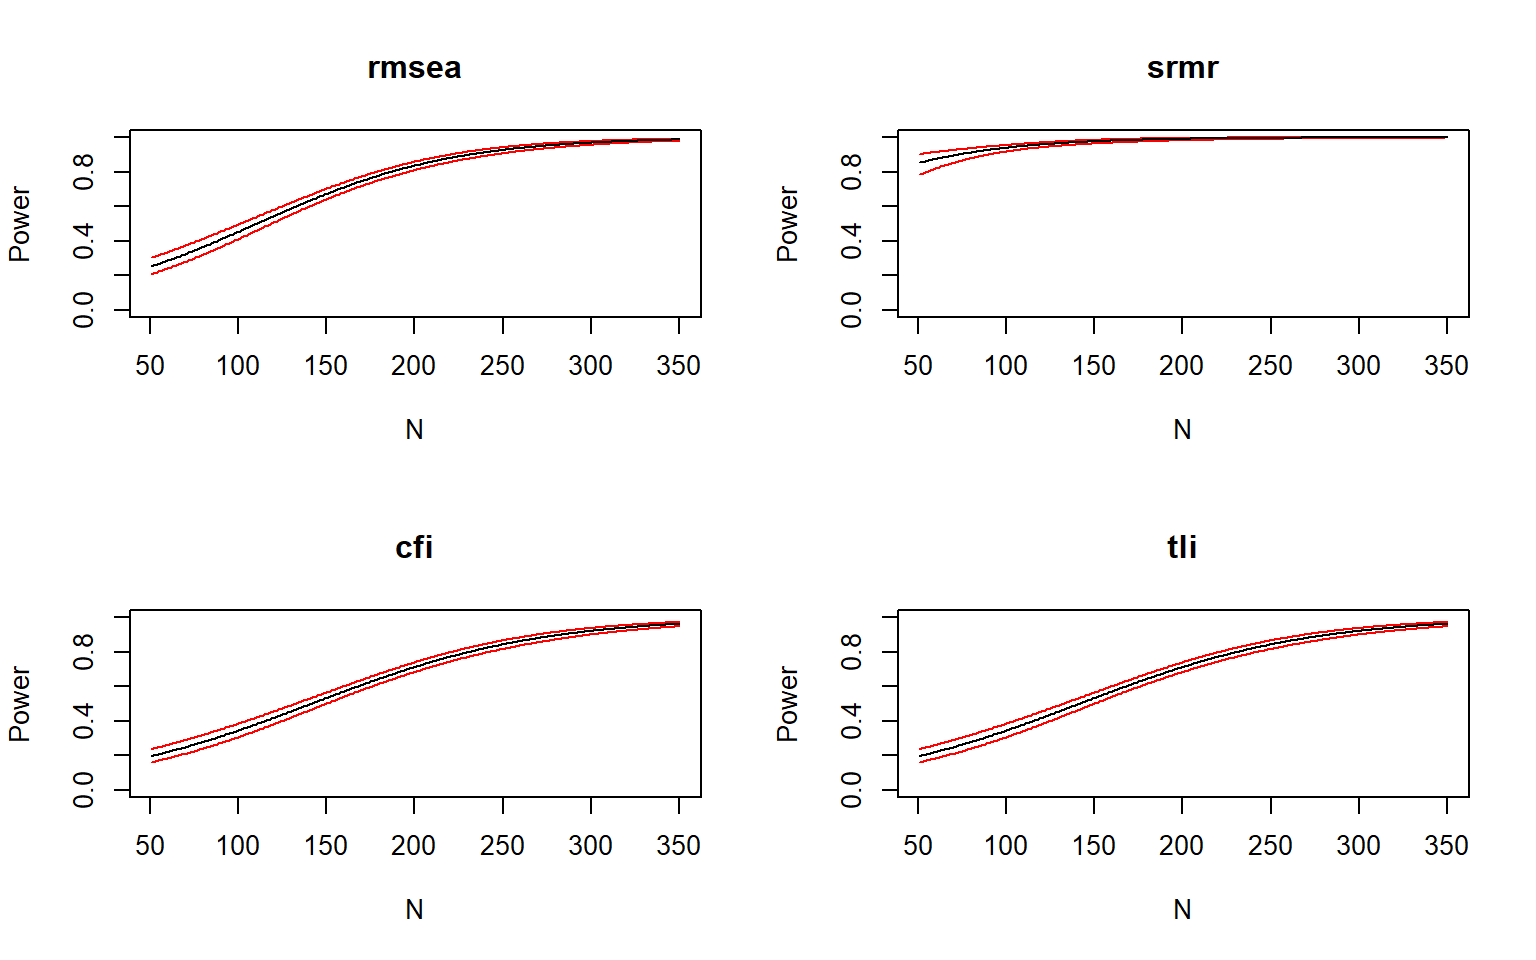
\includegraphics[keepaspectratio]{index_files/figure-latex/Scripts-AnalysisScripts-03_simulation_ideal-fig-power-curve-ideal-output-1.png}}

}

\caption{\label{fig-power-curve-ideal}Power curves for fit indices under
ideal conditions.}

\end{figure}%

\textsubscript{Source:
\href{https://phdpablo.github.io/cfa-power/Scripts/AnalysisScripts/03_simulation_ideal-preview.html\#cell-fig-power-curve-ideal}{Simulation
--- Ideal Conditions}}

Power increases monotonically with \(N\) for all four indices. At the
lower end of the sample-size sequence, every index falls below the
target threshold, indicating insufficient sensitivity. As \(N\) grows,
the curves diverge: some indices reach the \(0.80\) target earlier than
others, reflecting different degrees of sensitivity to the imposed
cross-loading misspecification. The most conservative planning decision
is therefore anchored in the last index to cross the target --- the
index whose detection requires the largest \(N\).

\begin{figure}[H]

\centering{

\pandocbounded{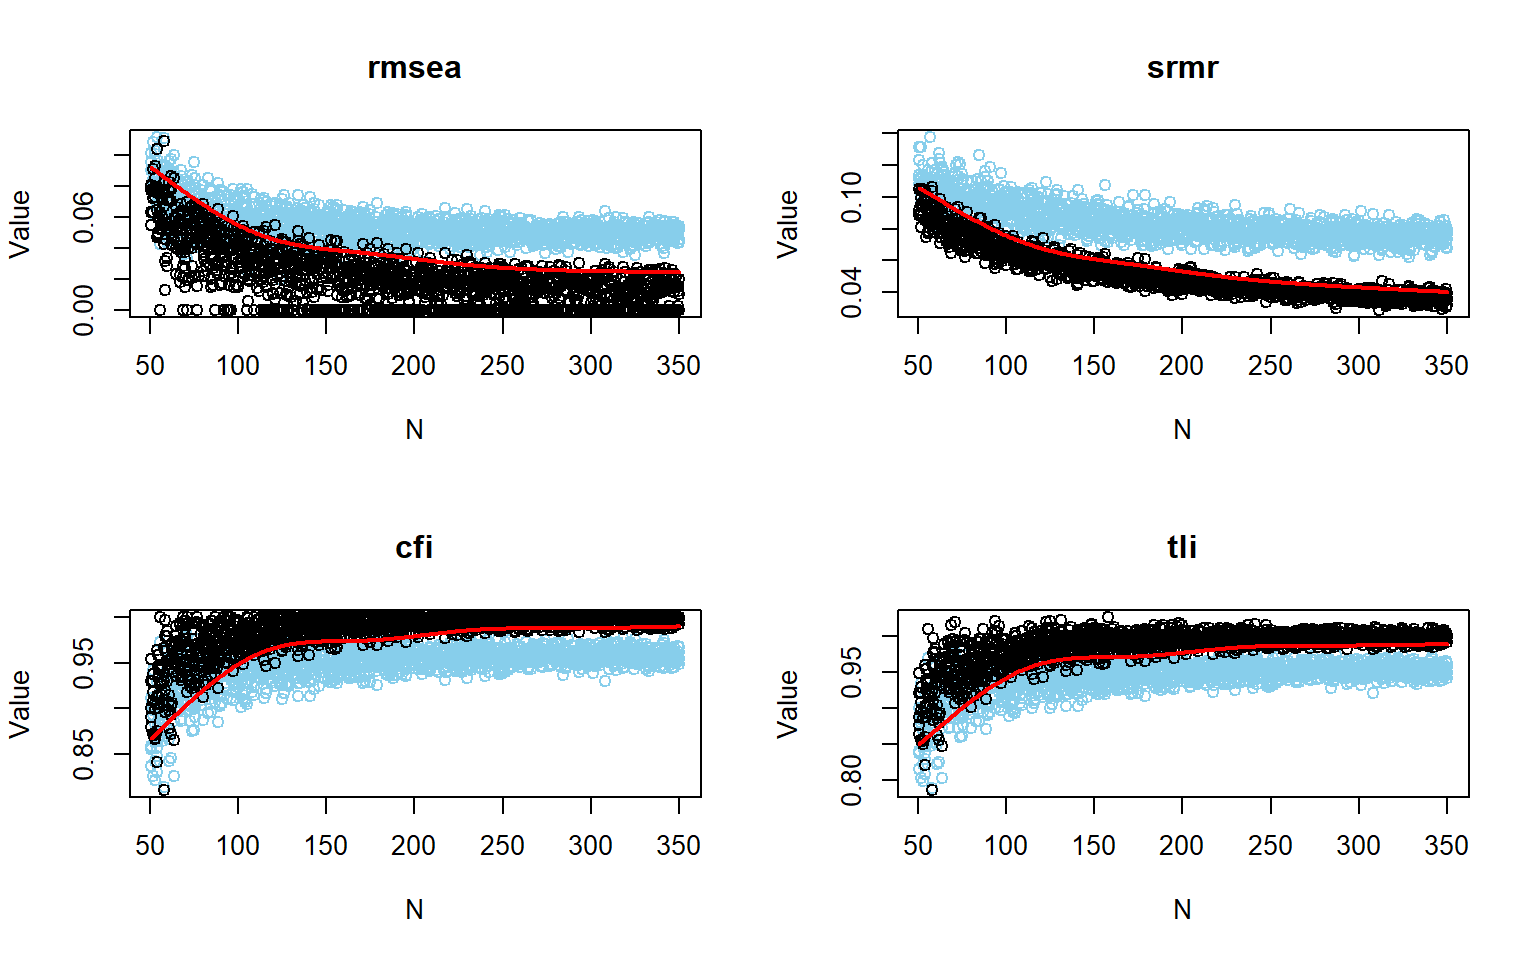
\includegraphics[keepaspectratio]{index_files/figure-latex/Scripts-AnalysisScripts-03_simulation_ideal-fig-fit-curve-ideal-output-1.png}}

}

\caption{\label{fig-fit-curve-ideal}Power curves for fit indices under
ideal conditions without logistic smoothing.}

\end{figure}%

\textsubscript{Source:
\href{https://phdpablo.github.io/cfa-power/Scripts/AnalysisScripts/03_simulation_ideal-preview.html\#cell-fig-fit-curve-ideal}{Simulation
--- Ideal Conditions}}

The Figure~\ref{fig-fit-curve-ideal} makes the discrimination mechanism
visible. At small \(N\), the sampling distributions of each fit index
under the reference and alternative conditions overlap substantially, so
the indices cannot reliably distinguish the two scenarios. As \(N\)
increases, the alternative-condition distribution shifts toward worse
fit while the reference distribution remains stable, widening the gap
between them. This growing separation is the empirical basis for the
power gains shown in the Figure~\ref{fig-power-curve-ideal}, and it
provides an intuitive picture of how fit indices work as decision
variables rather than mere descriptive summaries (McNeish \& Wolf, 2021;
Pornprasertmanit et al., 2021).

{

\begin{longtable}[]{@{}lcccc@{}}

\caption{\label{tbl-power-cutoff-ideal}Power and fit index cutoff values
under ideal conditions at N = 231.}

\tabularnewline

\toprule\noalign{}
& RMSEA & SRMR & CFI & TLI \\
\midrule\noalign{}
\endhead
\bottomrule\noalign{}
\endlastfoot
Power & 0.900 & 0.995 & 0.801 & 0.801 \\
Cutoff & 0.039 & 0.058 & 0.965 & 0.961 \\

\end{longtable}

}

\textsubscript{Source:
\href{https://phdpablo.github.io/cfa-power/Scripts/AnalysisScripts/03_simulation_ideal-preview.html\#cell-tbl-power-cutoff-ideal}{Simulation
--- Ideal Conditions}}

At \(N = 231\), power was 0.9 for RMSEA, 0.995 for SRMR, and 0.801 for
both CFI and TLI. The ordering SRMR \textgreater{} RMSEA \textgreater{}
CFI \(\approx\) TLI is consistent across the power curves. The empirical
cutoffs were 0.039 for RMSEA, 0.058 for SRMR, 0.965 for CFI, and 0.961
for TLI, defining the data-driven rejection boundaries at this \(N\).
Taken together, the results confirm that \(N = 231\) is sufficient for
all four indices to achieve at least \(0.80\) power in the ideal
scenario, with SRMR and RMSEA providing a comfortable margin and CFI/TLI
operating near the minimum threshold (Jobst et al., 2023; McNeish \&
Wolf, 2021).

\subsection{Traditional cutoff values for fit
indices}\label{traditional-cutoff-values-for-fit-indices}

When traditional thresholds are applied --- \(\text{RMSEA} \le .06\),
\(\text{CFI} \ge .95\), \(\text{TLI} \ge .95\), \(\text{SRMR} \le .06\)
--- power is defined as the proportion of replications in which the
misspecified model crosses those fixed boundaries in the direction of
worse fit. This mirrors common applied practice, but a key limitation is
that these thresholds were derived under specific simulation conditions
and may not be universally valid across different model structures and
sample sizes (Kyriazos, 2018; McNeish \& Wolf, 2021).

\begin{figure}[H]

\centering{

\pandocbounded{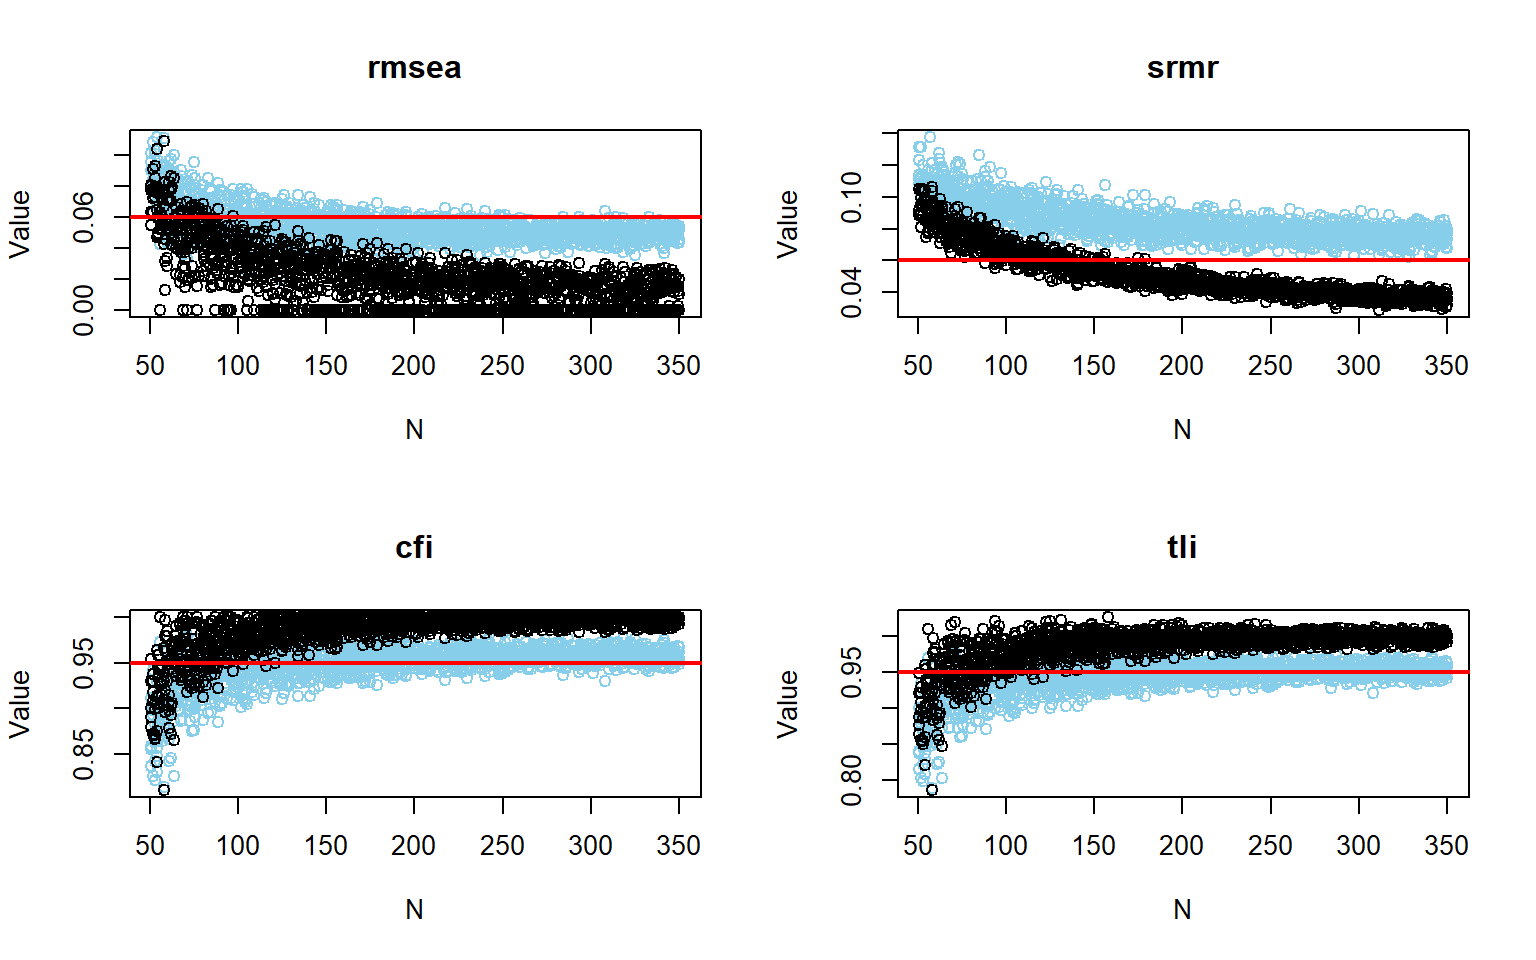
\includegraphics[keepaspectratio]{index_files/figure-latex/Scripts-AnalysisScripts-03_simulation_ideal-fig-fit-curve-traditional-output-1.png}}

}

\caption{\label{fig-fit-curve-traditional}Power curves using traditional
fit index cutoffs under ideal conditions.}

\end{figure}%

\textsubscript{Source:
\href{https://phdpablo.github.io/cfa-power/Scripts/AnalysisScripts/03_simulation_ideal-preview.html\#cell-fig-fit-curve-traditional}{Simulation
--- Ideal Conditions}}

The contrast with the empirical-cutoff results is instructive. SRMR is
the only index that achieves clear visual discrimination under the
traditional threshold, and only at \(N \approx 200\) or larger. RMSEA
shows some separation but would require a cutoff near \(0.04\) rather
than \(0.06\) to make a meaningful distinction in this figure. CFI and
TLI show essentially no discrimination at the \(0.95\) threshold because
both the reference and alternative point clouds cluster in the same
region throughout the sample-size range
(Figure~\ref{fig-fit-curve-traditional}). The
Table~\ref{tbl-power-cutoff-traditional-ideal} summarizes the power for
each fit index under the traditional cutoff values.

{

\begin{longtable}[]{@{}lcccc@{}}

\caption{\label{tbl-power-cutoff-traditional-ideal}Power for traditional
fit index cutoffs under ideal conditions at N = 231.}

\tabularnewline

\toprule\noalign{}
& CFI & TLI & RMSEA & SRMR \\
\midrule\noalign{}
\endhead
\bottomrule\noalign{}
\endlastfoot
Power & 0.381 & 0.579 & 0.153 & \textgreater{} 0.98 \\

\end{longtable}

}

\textsubscript{Source:
\href{https://phdpablo.github.io/cfa-power/Scripts/AnalysisScripts/03_simulation_ideal-preview.html\#cell-tbl-power-cutoff-traditional-ideal}{Simulation
--- Ideal Conditions}}

\subsection{Targeting specific
parameters}\label{targeting-specific-parameters}

The previous analyses focused on global fit. However, power is always
tied to a specific hypothesis, and different parameters within the same
model can require markedly different \(N\) to reach the same target
(Moshagen \& Bader, 2024; Wang, 2023). This section evaluates power at
the parameter level to identify which parts of the model are hardest to
recover and should therefore anchor the sample size decision.

In \texttt{simsem}, parameter-level summaries include relative bias,
standard-error bias, CI coverage, and detection power. These four
indicators are not redundant: a parameter may show high power while
still being poorly estimated, and estimation quality should always be
verified alongside detection rates (Pornprasertmanit et al., 2021; Wang
\& Rhemtulla, 2021).

{

\begin{longtable}[]{@{}
  >{\raggedright\arraybackslash}p{(\linewidth - 8\tabcolsep) * \real{0.3210}}
  >{\raggedright\arraybackslash}p{(\linewidth - 8\tabcolsep) * \real{0.1235}}
  >{\raggedright\arraybackslash}p{(\linewidth - 8\tabcolsep) * \real{0.1481}}
  >{\centering\arraybackslash}p{(\linewidth - 8\tabcolsep) * \real{0.1358}}
  >{\raggedright\arraybackslash}p{(\linewidth - 8\tabcolsep) * \real{0.2469}}@{}}

\caption{\label{tbl-param-estimate-ideal}Summary of parameter estimates
under ideal conditions.}

\tabularnewline

\toprule\noalign{}
\begin{minipage}[b]{\linewidth}\raggedright
Parameter
\end{minipage} & \begin{minipage}[b]{\linewidth}\raggedright
Rel Bias
\end{minipage} & \begin{minipage}[b]{\linewidth}\raggedright
Rel SE Bias
\end{minipage} & \begin{minipage}[b]{\linewidth}\centering
Coverage
\end{minipage} & \begin{minipage}[b]{\linewidth}\raggedright
Power (Not equal 0)
\end{minipage} \\
\midrule\noalign{}
\endhead
\bottomrule\noalign{}
\endlastfoot
psycho=\textasciitilde Q5 & -0.003 & -0.043 & 0.947 & 1.000 \\
psycho=\textasciitilde Q6 & -0.005 & -0.084 & 0.937 & 1.000 \\
psycho=\textasciitilde Q7 & -0.004 & -0.066 & 0.940 & 1.000 \\
psycho=\textasciitilde Q11 & -0.005 & -0.050 & 0.945 & 1.000 \\
psycho=\textasciitilde Q19 & -0.003 & 0.000 & 0.953 & 1.000 \\
psycho=\textasciitilde Q26 & -0.006 & -0.079 & 0.938 & 1.000 \\
physical=\textasciitilde Q3 & -0.011 & -0.063 & 0.947 & 1.000 \\
physical=\textasciitilde Q4 & -0.006 & -0.066 & 0.945 & 1.000 \\
physical=\textasciitilde Q10 & -0.010 & -0.062 & 0.947 & 1.000 \\
physical=\textasciitilde Q15 & 0.068 & -0.106 & 0.871 & 1.000 \\
physical=\textasciitilde Q16 & -0.011 & -0.061 & 0.941 & 1.000 \\
physical=\textasciitilde Q17 & -0.010 & -0.090 & 0.931 & 1.000 \\
physical=\textasciitilde Q18 & -0.011 & -0.077 & 0.938 & 1.000 \\
social=\textasciitilde Q20 & -0.004 & -0.050 & 0.941 & 1.000 \\
social=\textasciitilde Q21 & -0.003 & -0.025 & 0.952 & 1.000 \\
social=\textasciitilde Q22 & 0.002 & -0.048 & 0.943 & 1.000 \\
environment=\textasciitilde Q8 & 0.360 & -0.090 & 0.520 & 0.997 \\
environment=\textasciitilde Q9 & 0.105 & -0.051 & 0.879 & 0.999 \\
environment=\textasciitilde Q12 & -0.012 & -0.065 & 0.939 & 1.000 \\
environment=\textasciitilde Q13 & -0.010 & -0.080 & 0.942 & 1.000 \\
environment=\textasciitilde Q14 & -0.009 & -0.045 & 0.940 & 1.000 \\
environment=\textasciitilde Q23 & -0.010 & -0.075 & 0.939 & 1.000 \\
environment=\textasciitilde Q24 & -0.006 & -0.047 & 0.947 & 1.000 \\
environment=\textasciitilde Q25 & -0.011 & -0.059 & 0.940 & 1.000 \\
psycho\textasciitilde\textasciitilde physical & 0.039 & -0.069 & 0.941 &
0.751 \\
psycho\textasciitilde\textasciitilde social & -0.002 & -0.069 & 0.935 &
0.727 \\
psycho\textasciitilde\textasciitilde environment & 0.286 & -0.122 &
0.831 & 0.857 \\
physical\textasciitilde\textasciitilde social & 0.046 & -0.047 & 0.944 &
0.760 \\
physical\textasciitilde\textasciitilde environment & 0.239 & -0.091 &
0.875 & 0.839 \\
social\textasciitilde\textasciitilde environment & 0.038 & -0.070 &
0.931 & 0.736 \\
Q3\textasciitilde\textasciitilde Q4 & 0.007 & -0.050 & 0.944 & 0.775 \\
Q5\textasciitilde\textasciitilde Q5 & -0.012 & -0.043 & 0.944 & 0.999 \\
Q6\textasciitilde\textasciitilde Q6 & -0.017 & -0.039 & 0.934 & 1.000 \\
Q7\textasciitilde\textasciitilde Q7 & -0.020 & -0.071 & 0.929 & 0.993 \\
Q11\textasciitilde\textasciitilde Q11 & -0.014 & -0.073 & 0.926 &
1.000 \\
Q19\textasciitilde\textasciitilde Q19 & -0.014 & -0.050 & 0.933 &
1.000 \\
Q26\textasciitilde\textasciitilde Q26 & -0.018 & -0.038 & 0.933 &
1.000 \\
Q3\textasciitilde\textasciitilde Q3 & -0.012 & -0.059 & 0.935 & 1.000 \\
Q4\textasciitilde\textasciitilde Q4 & -0.015 & -0.040 & 0.944 & 1.000 \\
Q10\textasciitilde\textasciitilde Q10 & -0.008 & -0.044 & 0.934 &
1.000 \\
Q15\textasciitilde\textasciitilde Q15 & 0.105 & -0.068 & 0.896 &
1.000 \\
Q16\textasciitilde\textasciitilde Q16 & -0.011 & -0.055 & 0.934 &
1.000 \\
Q17\textasciitilde\textasciitilde Q17 & -0.008 & -0.084 & 0.934 &
0.999 \\
Q18\textasciitilde\textasciitilde Q18 & -0.008 & -0.010 & 0.949 &
1.000 \\
Q20\textasciitilde\textasciitilde Q20 & -0.004 & -0.091 & 0.943 &
0.848 \\
Q21\textasciitilde\textasciitilde Q21 & -0.015 & -0.042 & 0.946 &
0.991 \\
Q22\textasciitilde\textasciitilde Q22 & -0.018 & -0.050 & 0.933 &
1.000 \\
Q8\textasciitilde\textasciitilde Q8 & 0.536 & -0.058 & 0.136 & 1.000 \\
Q9\textasciitilde\textasciitilde Q9 & 0.028 & -0.059 & 0.944 & 1.000 \\
Q12\textasciitilde\textasciitilde Q12 & -0.001 & -0.036 & 0.943 &
1.000 \\
Q13\textasciitilde\textasciitilde Q13 & 0.004 & -0.042 & 0.936 &
1.000 \\
Q14\textasciitilde\textasciitilde Q14 & -0.002 & -0.085 & 0.937 &
1.000 \\
Q23\textasciitilde\textasciitilde Q23 & -0.001 & -0.029 & 0.945 &
1.000 \\
Q24\textasciitilde\textasciitilde Q24 & -0.013 & -0.055 & 0.937 &
1.000 \\
Q25\textasciitilde\textasciitilde Q25 & -0.007 & -0.058 & 0.942 &
1.000 \\

\end{longtable}

}

\textsubscript{Source:
\href{https://phdpablo.github.io/cfa-power/Scripts/AnalysisScripts/03_simulation_ideal-preview.html\#cell-tbl-param-estimate-ideal}{Simulation
--- Ideal Conditions}}

Primary factor loadings for \texttt{psycho}, \texttt{physical}, and
\texttt{social} recover very well: high power, minimal bias, modest SE
distortion, and coverage close to nominal. Two exceptions stand out. The
loading of \(Q8\) on \texttt{environment} and its residual variance are
easily detected but not well recovered --- the model would flag this
parameter as non-zero while still estimating it with noticeable
distortion. Item \(Q15\) shows a secondary warning on the same
dimensions. Among the latent parameters, interfactor covariances ---
particularly those involving \texttt{social} and \texttt{environment}
--- are harder to recover than loadings, with lower power and weaker
coverage. The residual covariance \(Q3 \sim\sim Q4\) stands out as the
most demanding residual parameter, behaving more like a latent
covariance than a measurement parameter in terms of inferential
difficulty.

The required \(N\) for each parameter follows directly from these
patterns (Jobst et al., 2023; Moshagen \& Bader, 2024), as shown in
Table~\ref{tbl-power-n-ideal}.

{

\begin{longtable}[]{@{}lc@{}}

\caption{\label{tbl-power-n-ideal}Sample size needed for 80\% power
under ideal conditions.}

\tabularnewline

\toprule\noalign{}
Parameter & N \\
\midrule\noalign{}
\endhead
\bottomrule\noalign{}
\endlastfoot
environment=\textasciitilde Q8 & 51 \\
environment=\textasciitilde Q9 & 51 \\
psycho\textasciitilde\textasciitilde physical & 200 \\
psycho\textasciitilde\textasciitilde social & 212 \\
psycho\textasciitilde\textasciitilde environment & 138 \\
physical\textasciitilde\textasciitilde social & 198 \\
physical\textasciitilde\textasciitilde environment & 148 \\
social\textasciitilde\textasciitilde environment & 208 \\
Q3\textasciitilde\textasciitilde Q4 & 181 \\
Q5\textasciitilde\textasciitilde Q5 & 51 \\
Q7\textasciitilde\textasciitilde Q7 & 51 \\
Q17\textasciitilde\textasciitilde Q17 & 51 \\
Q20\textasciitilde\textasciitilde Q20 & 143 \\
Q21\textasciitilde\textasciitilde Q21 & 51 \\

\end{longtable}

}

\textsubscript{Source:
\href{https://phdpablo.github.io/cfa-power/Scripts/AnalysisScripts/03_simulation_ideal-preview.html\#cell-tbl-power-n-ideal}{Simulation
--- Ideal Conditions}}

Many primary loadings and residual variances reach the target power at
the low end of the simulated range. Latent covariances and the residual
covariance \(Q3 \sim\sim Q4\) require substantially larger samples. In
practice, the sample size decision should be driven by the
hardest-to-detect parameters, not by the easiest ones --- a principle
that pushes the practical reference toward \(N \approx 200\) rather than
\(N \approx 50\) (Pornprasertmanit et al., 2021; Wang \& Rhemtulla,
2021). Specifically, the
\texttt{psycho\textasciitilde{}\textasciitilde{}social} covariance
requires \(N\) = 212, which sets the effective ceiling for
parameter-level planning in this model.

\subsection{Recovering population
parameters}\label{recovering-population-parameters}

\subsubsection{Parameter-level power under the naive
model}\label{parameter-level-power-under-the-naive-model}

Examining parameter recovery under the naive model serves as a
conservative benchmark for the measurement structure: because this
population assumes the weakest factor loadings
(\(\lambda \approx 0.40\)), indicator communalities are low, which
increases estimation uncertainty for the measurement parameters
({Mosqueira Taipe et al.}, 2026). Concurrently, its interfactor
correlations are moderate (\(\phi = 0.30\)). For detecting latent
covariances, a larger effect size (\(\phi = 0.30\)) requires a
substantially smaller sample size than a near-zero correlation, allowing
all six factor correlations to reach \(80\%\) power within \(N \le 90\)
(Pornprasertmanit et al., 2021; Wang \& Rhemtulla, 2021).

{

\begin{longtable}[]{@{}
  >{\raggedright\arraybackslash}p{(\linewidth - 10\tabcolsep) * \real{0.2989}}
  >{\raggedright\arraybackslash}p{(\linewidth - 10\tabcolsep) * \real{0.1034}}
  >{\centering\arraybackslash}p{(\linewidth - 10\tabcolsep) * \real{0.1264}}
  >{\centering\arraybackslash}p{(\linewidth - 10\tabcolsep) * \real{0.1264}}
  >{\centering\arraybackslash}p{(\linewidth - 10\tabcolsep) * \real{0.1954}}
  >{\raggedright\arraybackslash}p{(\linewidth - 10\tabcolsep) * \real{0.1264}}@{}}

\caption{\label{tbl-power-n-naive}Parameter estimates and required
sample size for 80\% power under naive conditions.}

\tabularnewline

\toprule\noalign{}
\begin{minipage}[b]{\linewidth}\raggedright
Parameter
\end{minipage} & \begin{minipage}[b]{\linewidth}\raggedright
Rel Bias
\end{minipage} & \begin{minipage}[b]{\linewidth}\centering
Rel SE Bias
\end{minipage} & \begin{minipage}[b]{\linewidth}\centering
Coverage
\end{minipage} & \begin{minipage}[b]{\linewidth}\centering
Power (Not equal 0)
\end{minipage} & \begin{minipage}[b]{\linewidth}\raggedright
Required N
\end{minipage} \\
\midrule\noalign{}
\endhead
\bottomrule\noalign{}
\endlastfoot
psycho\textasciitilde\textasciitilde physical & 0.140 & -0.944 & 0.913 &
0.793 & 180 \\
psycho\textasciitilde\textasciitilde social & -0.009 & -0.137 & 0.922 &
0.780 & 186 \\
psycho\textasciitilde\textasciitilde environment & -0.003 & -0.089 &
0.931 & 0.817 & 164 \\
physical\textasciitilde\textasciitilde social & 0.331 & -0.971 & 0.924 &
0.775 & 192 \\
physical\textasciitilde\textasciitilde environment & 0.141 & -0.932 &
0.929 & 0.793 & 178 \\
social\textasciitilde\textasciitilde environment & -0.014 & -0.123 &
0.928 & 0.780 & 184 \\
Q3\textasciitilde\textasciitilde Q4 & -0.013 & -0.130 & 0.932 & 0.845 &
143 \\

\end{longtable}

}

\textsubscript{Source:
\href{https://phdpablo.github.io/cfa-power/Scripts/AnalysisScripts/03_simulation_ideal-preview.html\#cell-tbl-power-n-naive}{Simulation
--- Ideal Conditions}}

Most factor loadings reach the \(0.80\) target with \(N < 60\),
confirming that the loading structure is not the binding constraint. The
binding constraint is the set of latent covariances. Their required
sample sizes are: \(\text{psycho} \sim\sim \text{physical}\) = 180,
\(\text{psycho} \sim\sim \text{social}\) = 186,
\(\text{psycho} \sim\sim \text{environment}\) = 164,
\(\text{physical} \sim\sim \text{social}\) = 192,
\(\text{physical} \sim\sim \text{environment}\) = 178, and
\(\text{social} \sim\sim \text{environment}\) = 184. The residual
covariance \(Q3 \sim\sim Q4\) requires \(N\) = 143, placing it between
the loadings and the latent covariances in difficulty. The largest
required \(N\) is \(\text{physical} \sim\sim \text{social}\) = 192,
which therefore governs the minimum sample size for the naive scenario.

\subsubsection{Parameter-level power under the optimistic
model}\label{parameter-level-power-under-the-optimistic-model}

Under the optimistic model, stronger loadings (\(\lambda \approx 0.80\))
and lower interfactor correlations (\(\phi = 0.08\)) yield two sharply
contrasting patterns ({Mosqueira Taipe et al.}, 2026). Because the
measurement structure is exceptionally strong, all primary factor
loadings and residual variances reach \(0.80\) power at the lowest
simulated sample size (\(N \le 51\)) with negligible bias. Conversely,
because the true interfactor correlations are very weak
(\(\phi = 0.08\)), detecting them as statistically different from zero
requires substantially larger samples: analytical power calculations
indicate that reaching \(80\%\) power for \(\phi = 0.08\) requires
\(N > 1,200\). Within the simulated sample-size range
(\(N \in [51, 350]\)), power for these correlations never crosses
\(0.80\), leading \texttt{findPower} to return \texttt{NA}.

{

\begin{longtable}[]{@{}
  >{\raggedright\arraybackslash}p{(\linewidth - 10\tabcolsep) * \real{0.1500}}
  >{\raggedright\arraybackslash}p{(\linewidth - 10\tabcolsep) * \real{0.1250}}
  >{\raggedright\arraybackslash}p{(\linewidth - 10\tabcolsep) * \real{0.1625}}
  >{\centering\arraybackslash}p{(\linewidth - 10\tabcolsep) * \real{0.1375}}
  >{\raggedright\arraybackslash}p{(\linewidth - 10\tabcolsep) * \real{0.2500}}
  >{\raggedright\arraybackslash}p{(\linewidth - 10\tabcolsep) * \real{0.1500}}@{}}

\caption{\label{tbl-power-n-opt}Parameter estimates and required sample
size for 80\% power under optimal conditions.}

\tabularnewline

\toprule\noalign{}
\begin{minipage}[b]{\linewidth}\raggedright
Parameter
\end{minipage} & \begin{minipage}[b]{\linewidth}\raggedright
Rel Bias
\end{minipage} & \begin{minipage}[b]{\linewidth}\raggedright
Rel SE Bias
\end{minipage} & \begin{minipage}[b]{\linewidth}\centering
Coverage
\end{minipage} & \begin{minipage}[b]{\linewidth}\raggedright
Power (Not equal 0)
\end{minipage} & \begin{minipage}[b]{\linewidth}\raggedright
Required N
\end{minipage} \\
\midrule\noalign{}
\endhead
\bottomrule\noalign{}
\endlastfoot
Q3\textasciitilde\textasciitilde Q4 & -0.008 & -0.082 & 0.934 & 0.85 &
139 \\

\end{longtable}

}

\textsubscript{Source:
\href{https://phdpablo.github.io/cfa-power/Scripts/AnalysisScripts/03_simulation_ideal-preview.html\#cell-tbl-power-n-opt}{Simulation
--- Ideal Conditions}}

Among parameters with finite required \(N\) above 60, only the residual
covariance \(Q3 \sim\sim Q4\) appears in Table~\ref{tbl-power-n-opt},
requiring \(N\) = 139. Rather than implying that the entire model is
powered at \(N = 51\), this analysis reveals that weak latent
correlations represent an acute bottleneck for parameter-level
hypothesis testing, even when measurement quality is optimal (Buchberger
et al., 2024; Pornprasertmanit et al., 2021). The contrast between the
naive and optimistic results demonstrates how sensitive \(N\)
recommendations are to the assumed population: the same model structure
implies very different requirements depending on which parameter set is
used, reinforcing the importance of sensitivity analyses across
population variants (Buchberger et al., 2024; Irmer et al., 2024).

\section{Monte Carlo Simulation: Realistic
Scenarios}\label{sec-sim-robust}

The ideal-condition analyses establish a theoretical baseline, but
actual data collection rarely conforms to multivariate normality with
complete observations. When non-normality or missing data are
anticipated, analytical power estimates may be optimistic, and the
required \(N\) should be reassessed under more realistic assumptions
(Feng \& Hancock, 2023; Wang, 2023). Monte Carlo simulation is
especially valuable here because it can encode precisely the data
conditions expected in practice --- including the missing-data
mechanism, the distributional shape, and the estimator --- and propagate
them through to the power estimate (Irmer et al., 2024; Schoemann et
al., 2014).

The goal of this section is not to replace the ideal-condition results
but to probe how sensitive they are to two common violations: missing
data and non-normality. Both analyses follow the same design logic as
before --- reference data from \texttt{popmodel}, alternative data from
\texttt{h1model}, analysis model \texttt{analyzemodel} --- so the
results remain directly comparable (Jobst et al., 2023; Moshagen \&
Bader, 2024).

\subsection{Missing Data (MCAR)}\label{sec-missing}

Missing data reduce the amount of usable information per participant and
therefore generally lower estimation efficiency and statistical power,
even when data are missing completely at random (MCAR) and the analysis
model handles missingness correctly via full information maximum
likelihood (Jak et al., 2021; Wolf et al., 2013). The relevant design
question is not only how many cases are planned but how much information
survives the anticipated missing-data process (Feng \& Hancock, 2023).

In this simulation, 10\% of observations are set missing at random prior
to each analysis. All other aspects of the design are unchanged from the
ideal-condition analysis.

\begin{figure}[H]

\centering{

\pandocbounded{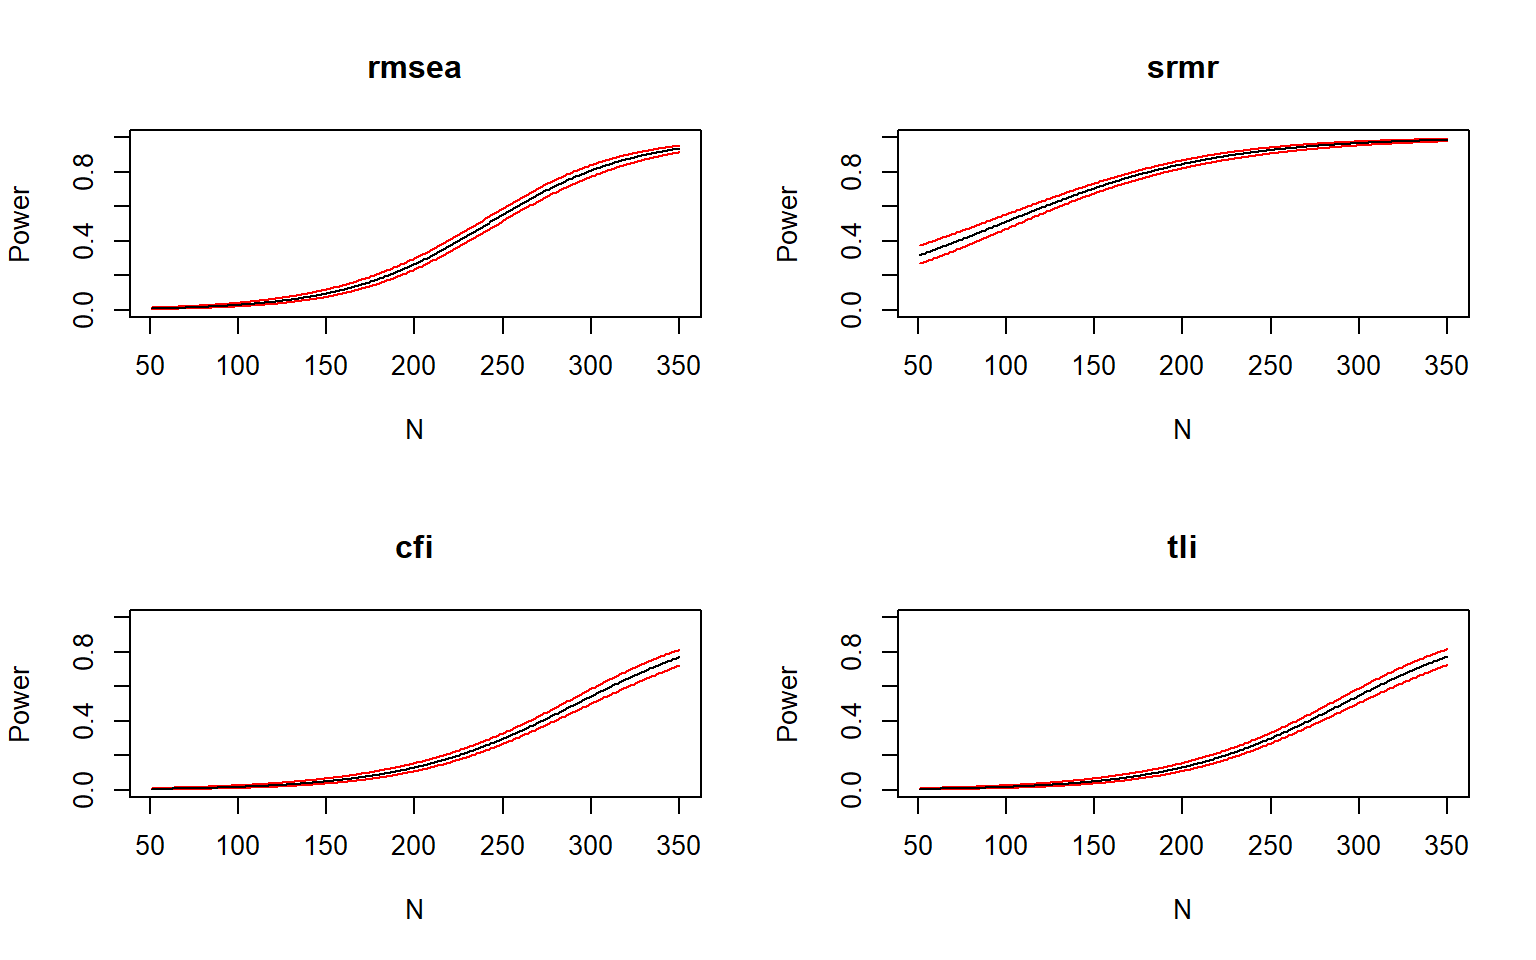
\includegraphics[keepaspectratio]{index_files/figure-latex/Scripts-AnalysisScripts-04_simulation_robust-fig-power-curve-missing-output-1.png}}

}

\caption{\label{fig-power-curve-missing}Power curves for fit indices
under missing data conditions.}

\end{figure}%

\textsubscript{Source:
\href{https://phdpablo.github.io/cfa-power/Scripts/AnalysisScripts/04_simulation_robust-preview.html\#cell-fig-power-curve-missing}{Simulation
--- Realistic Scenarios}}

\begin{figure}[H]

\centering{

\pandocbounded{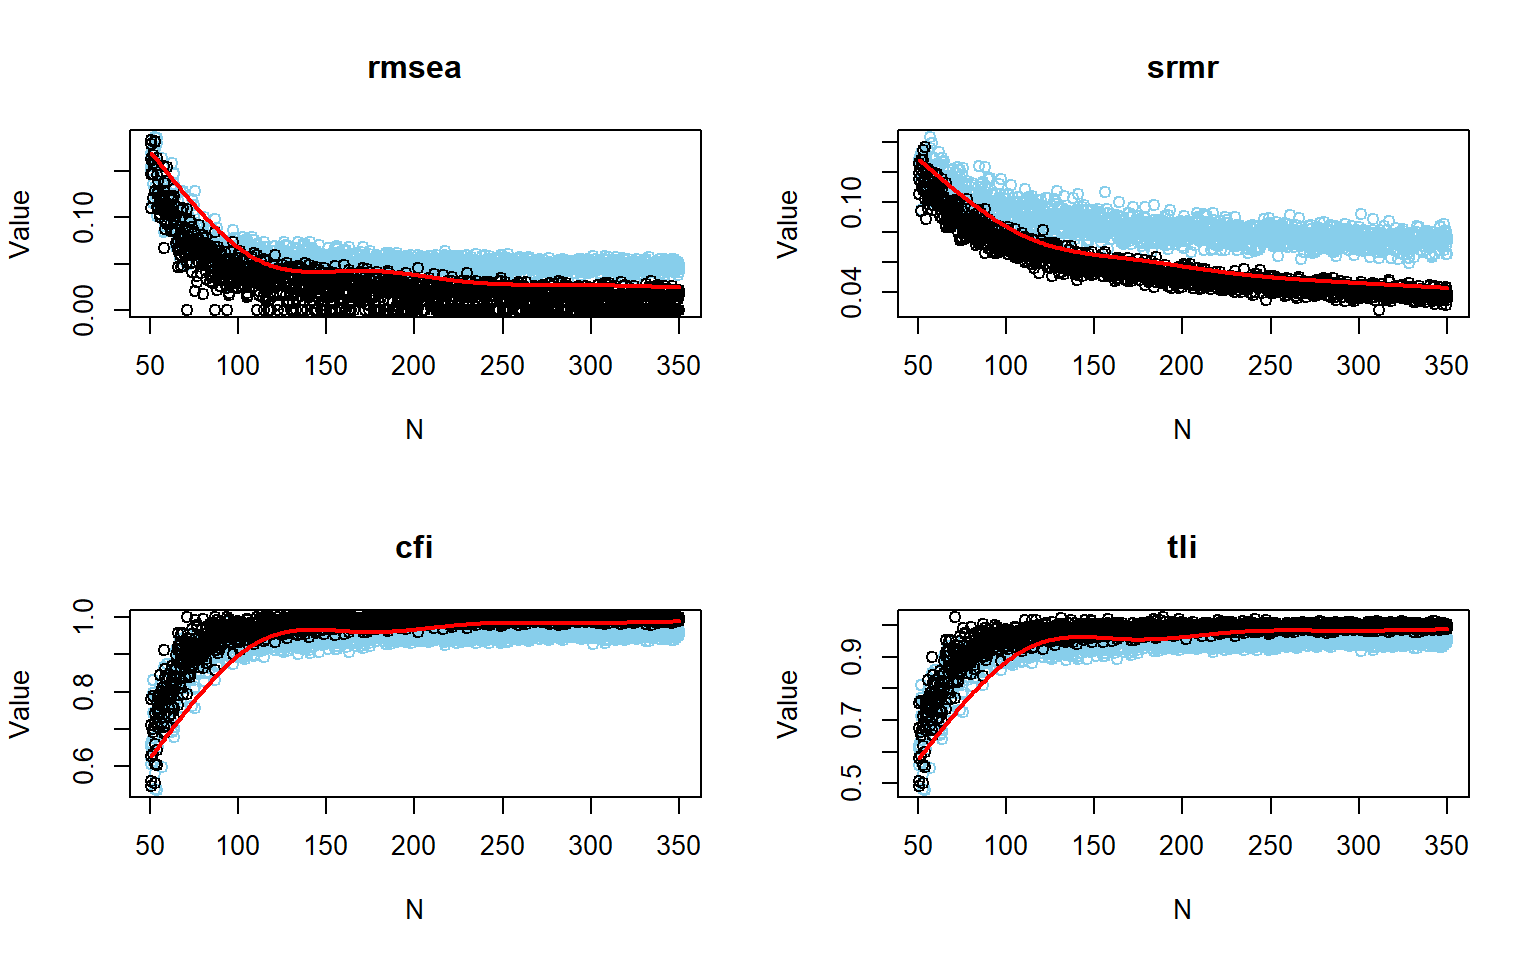
\includegraphics[keepaspectratio]{index_files/figure-latex/Scripts-AnalysisScripts-04_simulation_robust-fig-fit-curve-missing-output-1.png}}

}

\caption{\label{fig-fit-curve-missing}Power curves for fit indices under
missing data conditions without logistic smoothing.}

\end{figure}%

\textsubscript{Source:
\href{https://phdpablo.github.io/cfa-power/Scripts/AnalysisScripts/04_simulation_robust-preview.html\#cell-fig-fit-curve-missing}{Simulation
--- Realistic Scenarios}}

Both figures show the expected pattern: power curves shift rightward
relative to the ideal condition, requiring larger \(N\) to reach the
same thresholds. The separation between distributions in the raw
fit-index plots is less pronounced, especially for CFI and TLI, which
show more overlap at small and intermediate sample sizes.

{

\begin{longtable}[]{@{}lcccc@{}}

\caption{\label{tbl-power-cutoff-missing}Power and fit index cutoff
values under missing data conditions at N = 359.}

\tabularnewline

\toprule\noalign{}
& RMSEA & SRMR & CFI & TLI \\
\midrule\noalign{}
\endhead
\bottomrule\noalign{}
\endlastfoot
Power & 0.947 & 0.987 & 0.802 & 0.806 \\
Cutoff & 0.011 & 0.035 & 1.008 & 1.010 \\

\end{longtable}

}

\textsubscript{Source:
\href{https://phdpablo.github.io/cfa-power/Scripts/AnalysisScripts/04_simulation_robust-preview.html\#cell-tbl-power-cutoff-missing}{Simulation
--- Realistic Scenarios}}

At \(N = 359\), power was 0.947 for RMSEA, 0.987 for SRMR, 0.802 for
CFI, and 0.806 for TLI. SRMR remains the strongest index and RMSEA is
close behind; CFI and TLI are adequate but marginally so. The empirical
cutoffs were 0.011 for RMSEA, 0.035 for SRMR, 1.008 for CFI, and 1.01
for TLI. The values above \(1.00\) for CFI and TLI indicate that the
classification boundary from the simulation falls at the upper edge of
the index scale, which explains why their power is only marginally above
\(0.80\) at this \(N\) (McNeish \& Wolf, 2021). Comparing \(N = 231\)
(ideal) with \(N = 359\) (10\% MCAR) makes the information cost of
missing data concrete: approximately 128 additional participants are
needed to restore the same level of detection performance.

\subsection{Non-Normality}\label{sec-nonnormal}

Mild departures from normality --- skewness in the range \([-1, +1]\)
and excess kurtosis in the range \([1, 2]\) --- are common in applied
social science measurement and can affect the behavior of fit indices
even when robust estimators are used (Irmer et al., 2024; Kyriazos,
2018). This analysis evaluates how such departures alter the power
conclusions relative to the ideal condition.

\begin{figure}[H]

\centering{

\pandocbounded{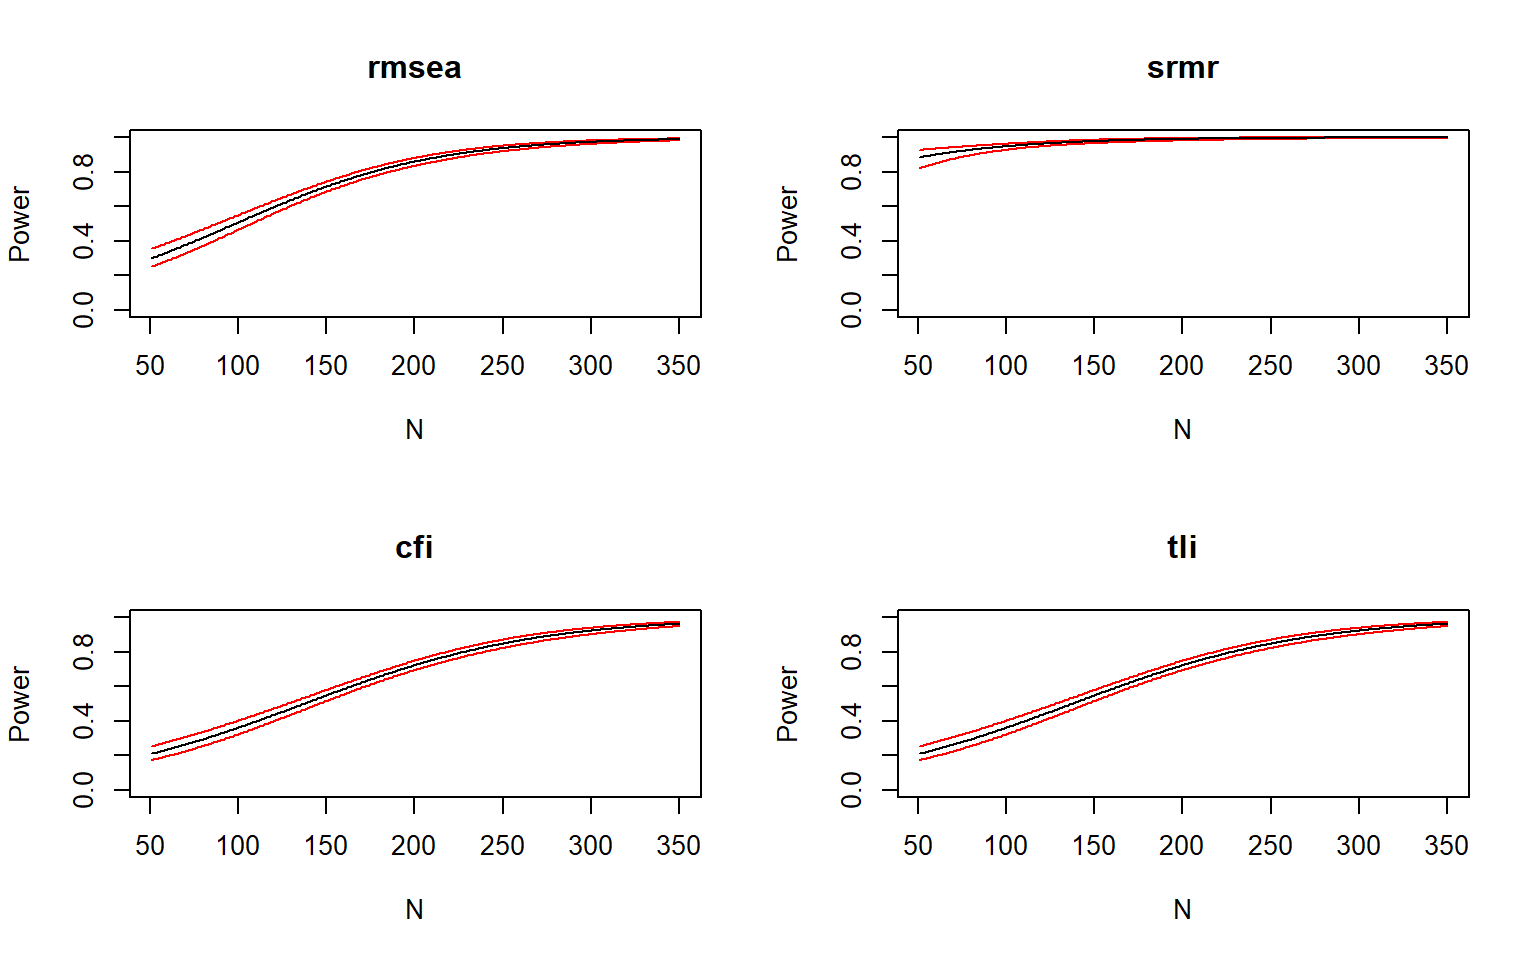
\includegraphics[keepaspectratio]{index_files/figure-latex/Scripts-AnalysisScripts-04_simulation_robust-fig-power-curve-nnorm-output-1.png}}

}

\caption{\label{fig-power-curve-nnorm}Power curves for fit indices under
non-normal conditions.}

\end{figure}%

\textsubscript{Source:
\href{https://phdpablo.github.io/cfa-power/Scripts/AnalysisScripts/04_simulation_robust-preview.html\#cell-fig-power-curve-nnorm}{Simulation
--- Realistic Scenarios}}

The ordering of sensitivity is stable: SRMR \(>\) RMSEA \(>\) CFI
\(\approx\) TLI. SRMR reaches near-ceiling power early in the
sample-size range; RMSEA follows steadily; CFI and TLI rise more slowly
and remain below the other two across most of the evaluated range.

\begin{figure}[H]

\centering{

\pandocbounded{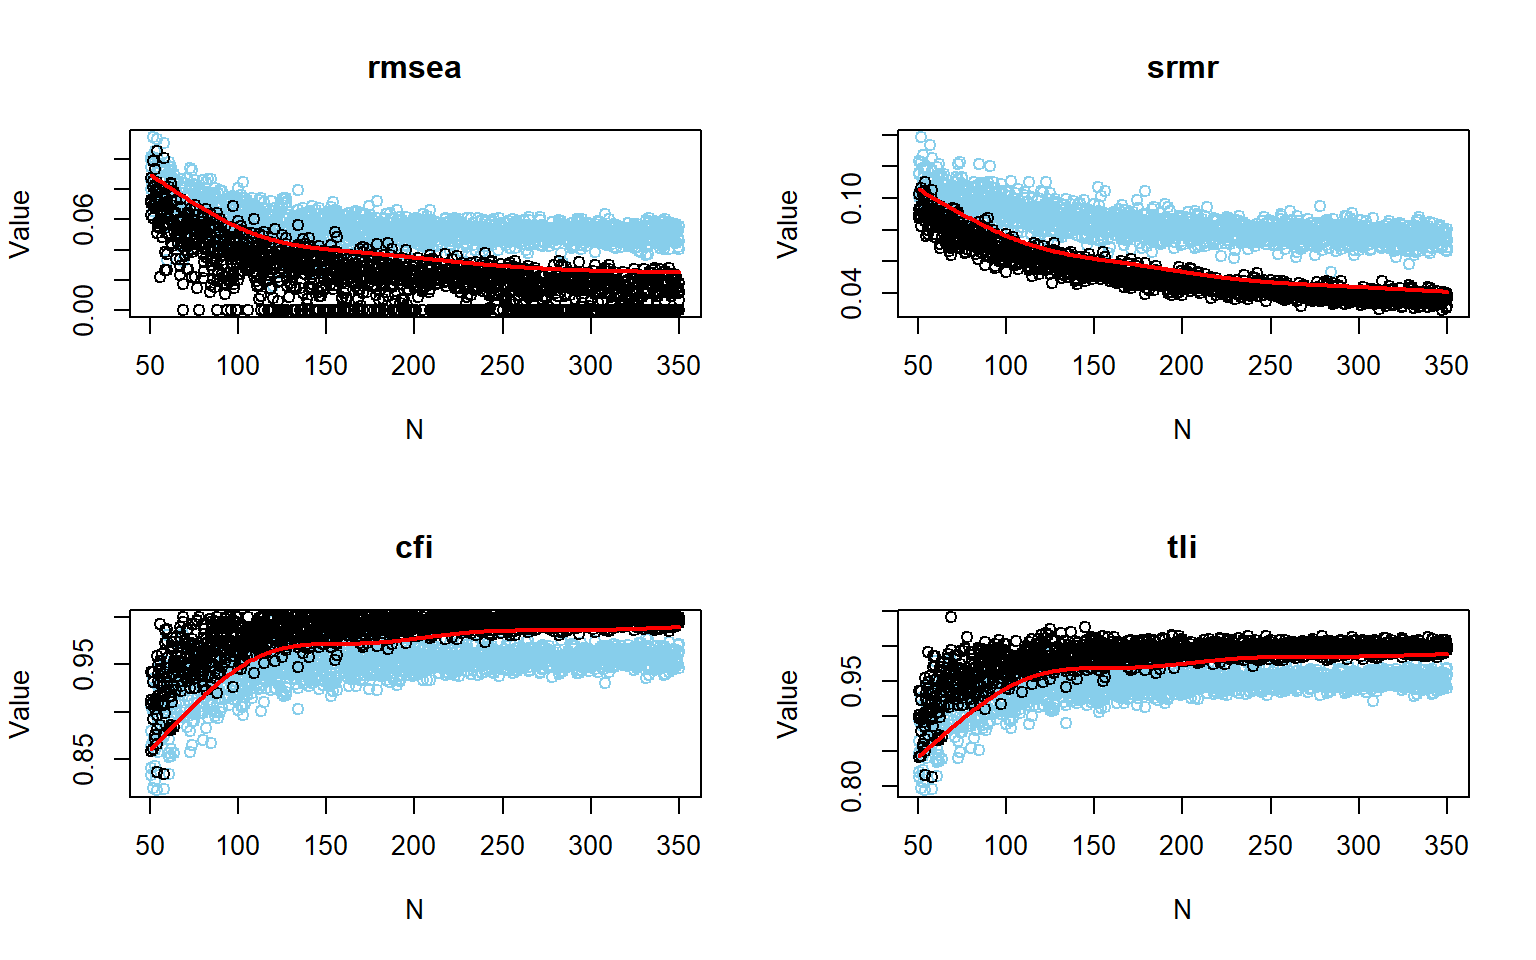
\includegraphics[keepaspectratio]{index_files/figure-latex/Scripts-AnalysisScripts-04_simulation_robust-fig-fit-curve-nnorm-output-1.png}}

}

\caption{\label{fig-fit-curve-nnorm}Power curves for fit indices under
non-normal conditions without logistic smoothing.}

\end{figure}%

\textsubscript{Source:
\href{https://phdpablo.github.io/cfa-power/Scripts/AnalysisScripts/04_simulation_robust-preview.html\#cell-fig-fit-curve-nnorm}{Simulation
--- Realistic Scenarios}}

The raw fit-index plots confirm the ordering. For RMSEA and SRMR, the
two point clouds are increasingly distinct as \(N\) grows; for CFI and
TLI, overlap is more visible at lower and intermediate sample sizes and
clears only at larger \(N\).

{

\begin{longtable}[]{@{}lcccc@{}}

\caption{\label{tbl-power-cutoff-nnorm}Power and fit index cutoff values
under non-normal conditions at N = 228.}

\tabularnewline

\toprule\noalign{}
& RMSEA & SRMR & CFI & TLI \\
\midrule\noalign{}
\endhead
\bottomrule\noalign{}
\endlastfoot
Power & 0.91 & 0.994 & 0.800 & 0.80 \\
Cutoff & 0.04 & 0.059 & 0.964 & 0.96 \\

\end{longtable}

}

\textsubscript{Source:
\href{https://phdpablo.github.io/cfa-power/Scripts/AnalysisScripts/04_simulation_robust-preview.html\#cell-tbl-power-cutoff-nnorm}{Simulation
--- Realistic Scenarios}}

At \(N = 228\), power was 0.91 for RMSEA, 0.994 for SRMR, 0.8 for CFI,
and 0.8 for TLI. Notably, this result is almost identical to the
ideal-condition estimate of \(N = 231\), suggesting that mild
non-normality introduces negligible additional cost under the current
design and model structure (Irmer et al., 2024). The empirical cutoffs
at \(N = 228\) were 0.04 (RMSEA), 0.059 (SRMR), 0.964 (CFI), and 0.96
(TLI), consistent with the discrimination patterns in the figures.

\subsection{Simulation with fixed N}\label{sec-scenarios-fixed}

Having established minimum sample size thresholds across individual
analytical and simulation conditions --- where requirements largely
converged between \(N = 100\) and \(N = 231\) --- the planning focus
naturally shifts from searching for the smallest sufficient \(N\) to
evaluating a candidate recruitment target. In applied research, sample
sizes are frequently shaped by budgetary, temporal, and logistical
feasibility.

Fixing \(N = 250\) represents a realistic, well-powered target sample
size that comfortably exceeds both the ideal (\(N = 231\)) and
non-normal (\(N = 228\)) benchmarks. This section subjects this planned
sample size to a rigorous Monte Carlo stress test: evaluating 1,000
independent replications under compound realistic disturbances
simultaneously (10\% MCAR missing data and mild non-normality with
robust MLR estimation). The goal is to determine whether a planned study
with \(N = 250\) reliably discriminates the true from the misspecified
model under combined real-world imperfections.

This step also highlights the practical difference between empirical and
traditional fit criteria. Empirical cutoffs are calibrated to the actual
sampling distribution of the fitted model; traditional cutoffs are
generic conventions. The two approaches can lead to very different
conclusions about adequacy (McNeish \& Wolf, 2021; Pornprasertmanit et
al., 2021).

\begin{figure}[H]

\centering{

\pandocbounded{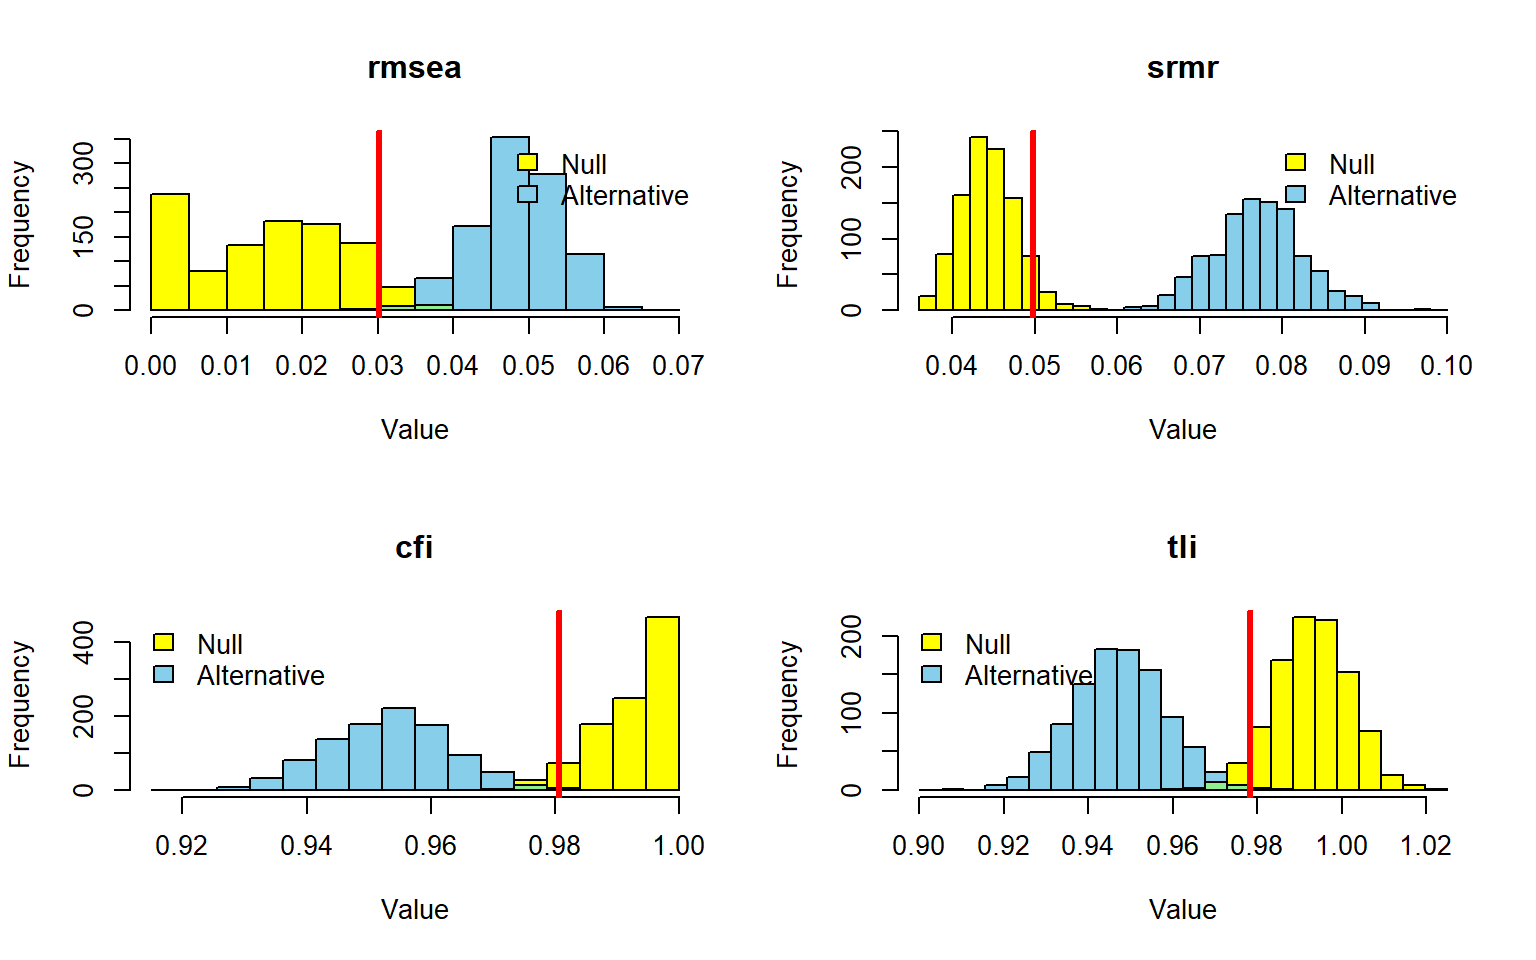
\includegraphics[keepaspectratio]{index_files/figure-latex/Scripts-AnalysisScripts-05_model_comparison-fig-power-curve-fixed-output-1.png}}

}

\caption{\label{fig-power-curve-fixed}Power curves for fit indices with
fixed sample size.}

\end{figure}%

\textsubscript{Source:
\href{https://phdpablo.github.io/cfa-power/Scripts/AnalysisScripts/05_model_comparison-preview.html\#cell-fig-power-curve-fixed}{Simulation
--- Fixed N}}

With \(N = 250\), the main analysis achieves power = 1.000 for all four
fit indices using empirical cutoffs. The distributions of the reference
and alternative conditions are completely separated in every panel,
confirming that this sample size provides essentially perfect
discrimination under the target design (Liang \& Sterba, 2024; Moshagen
\& Bader, 2024). The empirical cutoffs at \(N = 250\) serve as
data-driven benchmarks for this specific population-analysis model
combination, and their values (Table~\ref{tbl-power-cutoff-fixed})
differ noticeably from conventional thresholds --- which underscores the
value of deriving rejection rules from the simulation rather than from
generic recommendations.

{

\begin{longtable}[]{@{}lcccc@{}}

\caption{\label{tbl-power-cutoff-fixed}Power and fit index cutoff values
with fixed sample size.}

\tabularnewline

\toprule\noalign{}
& RMSEA & SRMR & CFI & TLI \\
\midrule\noalign{}
\endhead
\bottomrule\noalign{}
\endlastfoot
Power & 0.998 & 1.00 & 0.997 & 0.997 \\
Cutoff & 0.030 & 0.05 & 0.981 & 0.978 \\

\end{longtable}

}

\textsubscript{Source:
\href{https://phdpablo.github.io/cfa-power/Scripts/AnalysisScripts/05_model_comparison-preview.html\#cell-tbl-power-cutoff-fixed}{Simulation
--- Fixed N}}

\subsubsection{Power analysis with traditional
cutoffs}\label{power-analysis-with-traditional-cutoffs}

Applying traditional rule-of-thumb thresholds to the same fixed-\(N\)
simulation produces a strikingly different picture. Power remains high
for SRMR, falls substantially for CFI and TLI, and drops to zero for
RMSEA --- not because the sample is inadequate, but because the
conventional \(\text{RMSEA} \le 0.05\) threshold is misaligned with the
empirical distribution of this specific model (Kyriazos, 2018; McNeish
\& Wolf, 2021). This contrast is one of the clearest illustrations in
this tutorial of why power conclusions depend on how the rejection
criterion is defined, not only on \(N\).

\begin{figure}[H]

\centering{

\pandocbounded{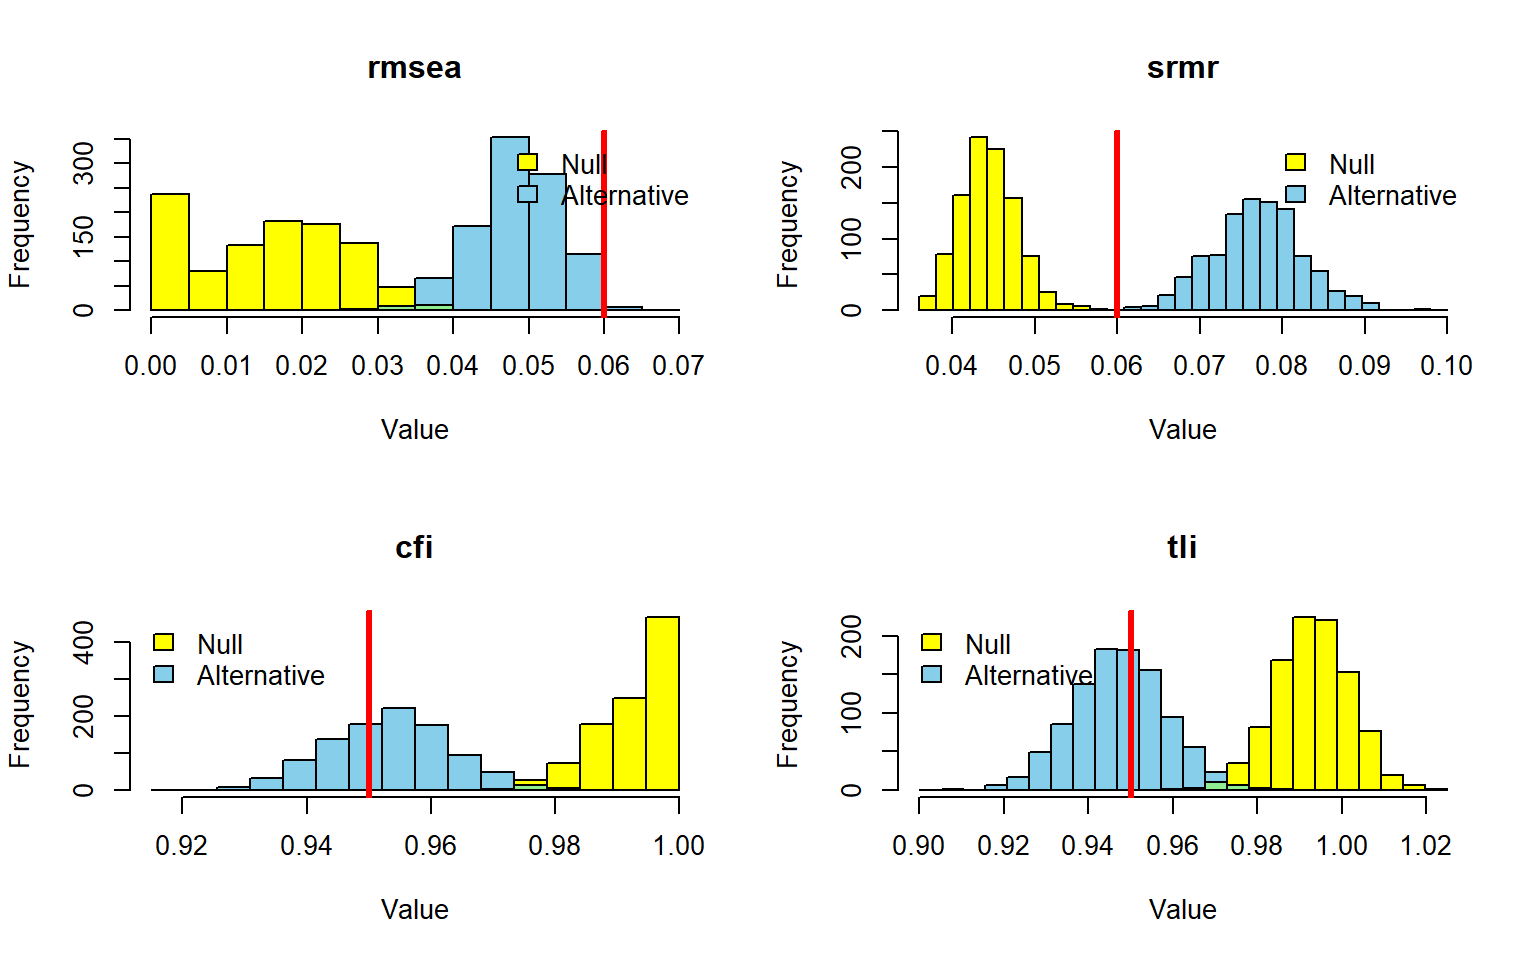
\includegraphics[keepaspectratio]{index_files/figure-latex/Scripts-AnalysisScripts-05_model_comparison-fig-curve-fixed-traditional-output-1.png}}

}

\caption{\label{fig-curve-fixed-traditional}Power curves using
traditional fit index cutoffs with fixed sample size.}

\end{figure}%

\textsubscript{Source:
\href{https://phdpablo.github.io/cfa-power/Scripts/AnalysisScripts/05_model_comparison-preview.html\#cell-fig-curve-fixed-traditional}{Simulation
--- Fixed N}}

{

\begin{longtable}[]{@{}lcccc@{}}

\caption{\label{tbl-power-cutoff-traditional-fixed}Power for traditional
fit index cutoffs with fixed sample size.}

\tabularnewline

\toprule\noalign{}
& CFI & TLI & RMSEA & SRMR \\
\midrule\noalign{}
\endhead
\bottomrule\noalign{}
\endlastfoot
Power & 0.354 & 0.587 & 0.007 & 0.999 \\

\end{longtable}

}

\textsubscript{Source:
\href{https://phdpablo.github.io/cfa-power/Scripts/AnalysisScripts/05_model_comparison-preview.html\#cell-tbl-power-cutoff-traditional-fixed}{Simulation
--- Fixed N}}

Taken together, the fixed-\(N\) results support \(N = 250\) as a
conservative, stable design choice for the main comparison: it delivers
perfect discrimination when empirical cutoffs are used, and its failures
under traditional cutoffs reveal a limitation of those cutoffs rather
than of the design itself (Liang \& Sterba, 2024; Pornprasertmanit et
al., 2021).

\section{Post Hoc Power Analysis}\label{sec-post-hoc}

Post hoc power analysis evaluates the detection capacity of a study
design after the data have been collected, using the observed \(N\), the
fitted model, and a specified reference structure. In SEM, this is
meaningful only with respect to a clearly defined comparison: power is
always the probability of rejecting a specific model under a specific
alternative, not a general property of a dataset or a software routine
(Jobst et al., 2023; Moshagen \& Bader, 2024). In this section, we
evaluate post hoc power against an empirical dataset from Mendeley
(Rogers, 2022), fitting \texttt{analyzemodel} to real WHOQOL-BREF data
and assessing how reliably the collected \(N\) would have rejected
meaningful misspecification.

\subsection{With Simulation}\label{with-simulation}

The simulation-based strategy first fits the analysis model to the real
data to obtain an empirically grounded reference structure. It then
generates data from both the null model and the alternative model at the
observed \(N\) and quantifies how well the fit indices separate the two
conditions. This approach is particularly informative when the effect of
interest is defined in model terms, because the full parameterization
--- loadings, residual structure, latent correlations --- shapes the
discrepancy and therefore the power estimate (Feng \& Hancock, 2023;
Wang \& Rhemtulla, 2021).

\begin{figure}[H]

\centering{

\pandocbounded{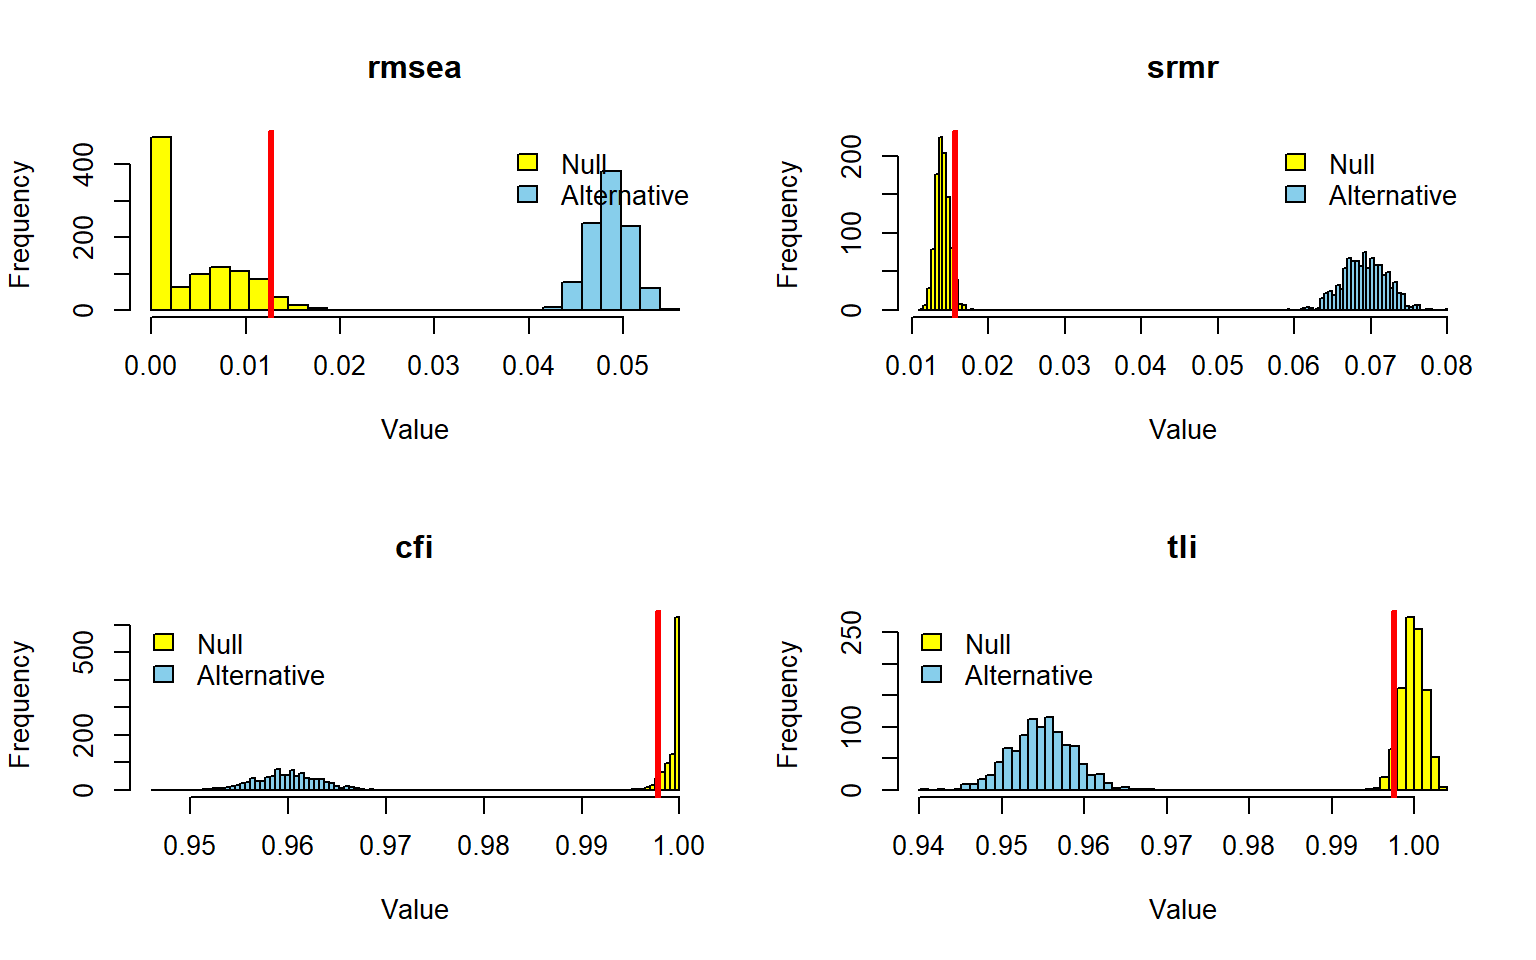
\includegraphics[keepaspectratio]{index_files/figure-latex/Scripts-AnalysisScripts-06_posthoc-fig-posthoc-plotpower-output-1.png}}

}

\caption{\label{fig-posthoc-plotpower}Power curve for post hoc analysis
based on simulation.}

\end{figure}%

\textsubscript{Source:
\href{https://phdpablo.github.io/cfa-power/Scripts/AnalysisScripts/06_posthoc-preview.html\#cell-fig-posthoc-plotpower}{Post
Hoc Power Analysis}}

{

\begin{longtable}[]{@{}cccc@{}}

\caption{\label{tbl-posthoc-power}Power for post hoc analysis based on
simulation.}

\tabularnewline

\toprule\noalign{}
RMSEA & SRMR & CFI & TLI \\
\midrule\noalign{}
\endhead
\bottomrule\noalign{}
\endlastfoot
1 & 1 & 1 & 1 \\

\end{longtable}

}

\textsubscript{Source:
\href{https://phdpablo.github.io/cfa-power/Scripts/AnalysisScripts/06_posthoc-preview.html\#cell-tbl-posthoc-power}{Post
Hoc Power Analysis}}

All four fit indices reached power equal to \(1.00\). In the figure,
every panel shows complete separation between the null and alternative
distributions, with the red cutoff line falling cleanly between them and
no visible overlap. For RMSEA, the null distribution concentrates near
zero while the alternative is centered around \(0.05\). For SRMR, the
null clusters near \(0.01\)--\(0.02\) and the alternative near
\(0.06\)--\(0.08\). For CFI and TLI, the null is close to \(1.00\) and
the alternative centers around \(0.95\)--\(0.97\). The complete
discrimination in every panel confirms that the observed \(N\) would
have been fully adequate to detect the target misspecification
(Pornprasertmanit et al., 2021). Note that some indices are operating
below their conventional thresholds, which is a consequence of the
empirical cutoffs derived from the null distribution in this specific
setting --- not an indication that model fit is poor.

\subsection{With Analytical Solutions}\label{with-analytical-solutions}

Analytical post hoc power expresses the effect through \(F_0\) or RMSEA
and links it to the noncentrality-based framework of the
likelihood-ratio test. This is computationally immediate and free from
Monte Carlo sampling error, making it the preferred first-pass approach
when the asymptotic assumptions underlying the chi-square test are
credible (Jak et al., 2021; Moshagen \& Bader, 2024). Two specifications
are compared here, illustrating a spectrum from the most generic to the
most substantively specific formulation.

\subsubsection{Model-free specification}\label{model-free-specification}

The first specification supplies \(\text{RMSEA} = 0.05\) directly,
treating misspecification as a generic level of global misfit per degree
of freedom. This makes the analysis comparable across SEM families
sharing the same \(df\), but it abstracts away from the particular
covariance structure of the WHOQOL-BREF model (Jak et al., 2021;
MacCallum et al., 1996).

{

\begin{longtable}[]{@{}
  >{\raggedright\arraybackslash}p{(\linewidth - 4\tabcolsep) * \real{0.5065}}
  >{\centering\arraybackslash}p{(\linewidth - 4\tabcolsep) * \real{0.3247}}
  >{\raggedleft\arraybackslash}p{(\linewidth - 4\tabcolsep) * \real{0.1429}}@{}}

\caption{\label{tbl-posthoc-rmsea}Analytical post hoc power parameters
for RMSEA = 0.05}

\tabularnewline

\toprule\noalign{}
\begin{minipage}[b]{\linewidth}\raggedright
Metric
\end{minipage} & \begin{minipage}[b]{\linewidth}\centering
Symbol
\end{minipage} & \begin{minipage}[b]{\linewidth}\raggedleft
Value
\end{minipage} \\
\midrule\noalign{}
\endhead
\bottomrule\noalign{}
\endlastfoot
Population discrepancy & \(F_0\) & 0.613 \\
Root mean square error of approximation & \(\text{RMSEA}\) & 0.050 \\
McDonald centrality index & \(Mc\) & 0.736 \\
Goodness-of-fit index & \(\text{GFI}\) & 0.951 \\
Adjusted goodness-of-fit index & \(\text{AGFI}\) & 0.941 \\
Degrees of freedom & \(df\) & 245 \\
Observed sample size & \(N\) & 1047 \\
Critical chi-square & \(\chi^2_{\text{crit}}\) & 282.511 \\
Noncentrality parameter & \(\lambda\) & 640.675 \\
Significance level (alpha) & \(\alpha\) & 0.050 \\
Type II error rate (beta) & \(\beta\) & 3.07e-47 \\
Statistical power & \(1 - \beta\) & \textgreater{} 0.9999 \\

\end{longtable}

}

\textsubscript{Source:
\href{https://phdpablo.github.io/cfa-power/Scripts/AnalysisScripts/06_posthoc-preview.html\#cell-tbl-posthoc-rmsea}{Post
Hoc Power Analysis}}

The post hoc power parameters in Table~\ref{tbl-posthoc-rmsea}
demonstrate that with \(F_0\) = 0.613, \(\text{RMSEA}\) = 0.05, \(df\) =
245, and \(N\) = 1047, the noncentrality parameter reached
\(\text{NCP}\) = 640.675, far exceeding the critical value
\(\chi^2_{\text{crit}}\) = 282.511. Power was effectively 1. As
illustrated in Figure~\ref{fig-posthoc-rmsea}, the noncentral \(\chi^2\)
curve lies far to the right of the critical value, and the shaded
\(\beta\) region is negligible (Jobst et al., 2023; MacCallum et al.,
1996).

\begin{figure}[H]

\centering{

\pandocbounded{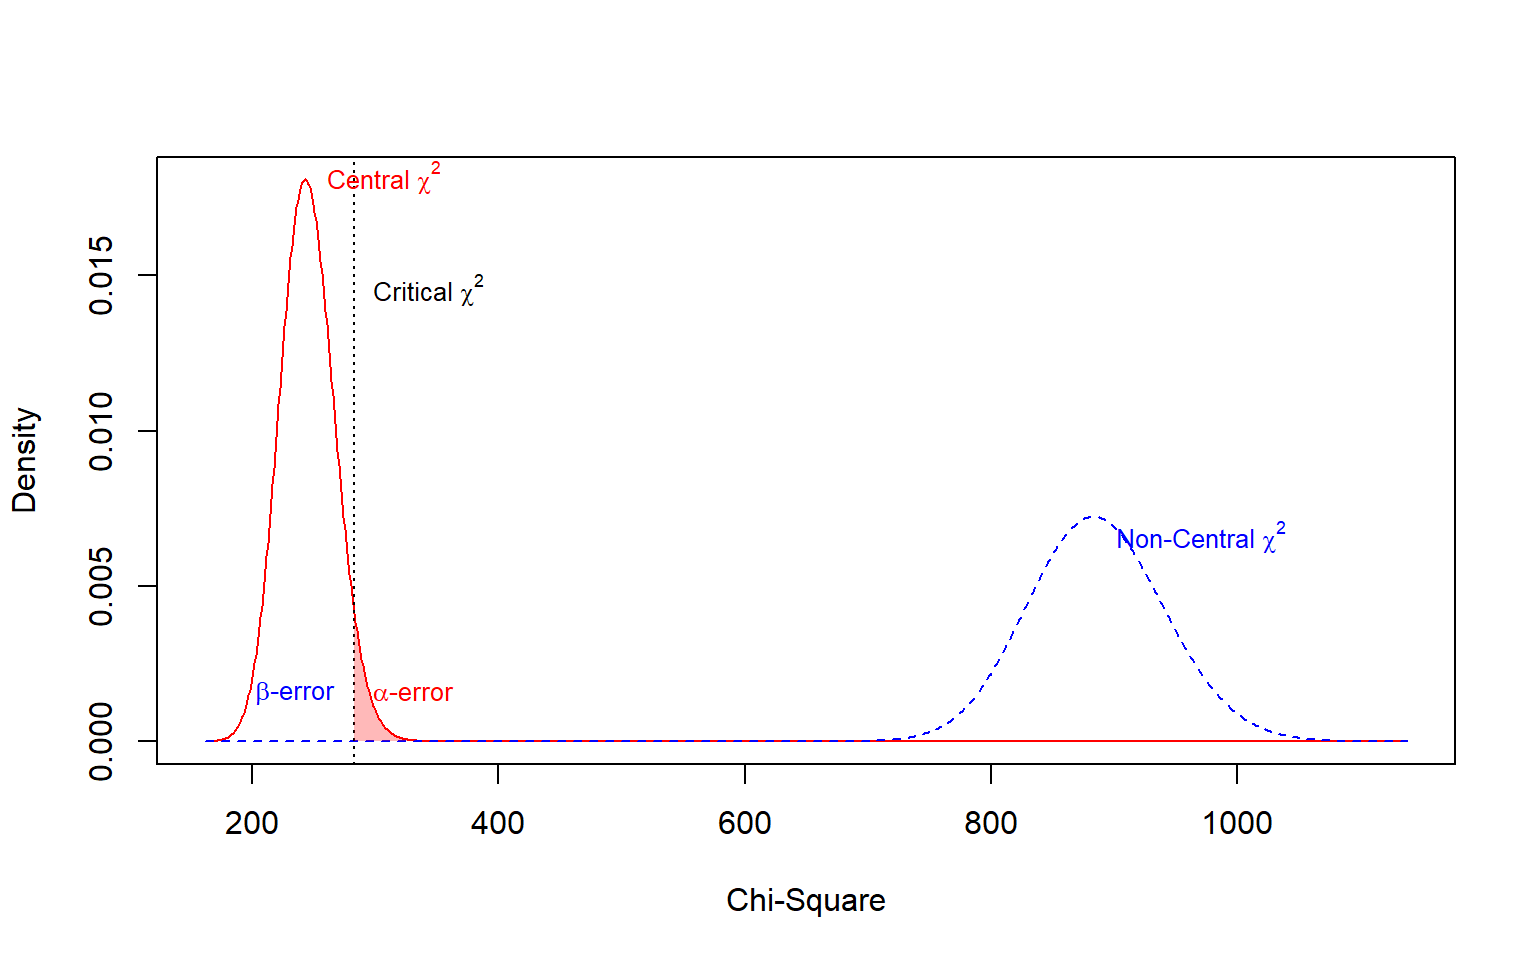
\includegraphics[keepaspectratio]{index_files/figure-latex/Scripts-AnalysisScripts-06_posthoc-fig-posthoc-rmsea-output-1.png}}

}

\caption{\label{fig-posthoc-rmsea}Post hoc power analysis for RMSEA =
0.05.}

\end{figure}%

\textsubscript{Source:
\href{https://phdpablo.github.io/cfa-power/Scripts/AnalysisScripts/06_posthoc-preview.html\#cell-fig-posthoc-rmsea}{Post
Hoc Power Analysis}}

\subsubsection{Model-based specification: global
fit}\label{model-based-specification-global-fit}

The second specification derives the effect from the discrepancy between
\texttt{h1model} (incorporating the cross-loadings) and the fitted
analysis model, evaluating the null model against the saturated model.
This tests global fit rather than an isolated restriction, so it is
sensitive to any source of misspecification in the analysis model, not
only the cross-loadings (Moshagen \& Bader, 2024; Wang, 2023).

{

\begin{longtable}[]{@{}
  >{\raggedright\arraybackslash}p{(\linewidth - 4\tabcolsep) * \real{0.5065}}
  >{\centering\arraybackslash}p{(\linewidth - 4\tabcolsep) * \real{0.3247}}
  >{\raggedleft\arraybackslash}p{(\linewidth - 4\tabcolsep) * \real{0.1429}}@{}}

\caption{\label{tbl-posthoc-realmodel}Analytical post hoc power
parameters for empirical fitted model}

\tabularnewline

\toprule\noalign{}
\begin{minipage}[b]{\linewidth}\raggedright
Metric
\end{minipage} & \begin{minipage}[b]{\linewidth}\centering
Symbol
\end{minipage} & \begin{minipage}[b]{\linewidth}\raggedleft
Value
\end{minipage} \\
\midrule\noalign{}
\endhead
\bottomrule\noalign{}
\endlastfoot
Population discrepancy & \(F_0\) & 0.579 \\
Root mean square error of approximation & \(\text{RMSEA}\) & 0.049 \\
McDonald centrality index & \(Mc\) & 0.749 \\
Goodness-of-fit index & \(\text{GFI}\) & 0.954 \\
Adjusted goodness-of-fit index & \(\text{AGFI}\) & 0.944 \\
Standardized root mean square residual & \(\text{SRMR}\) & 0.067 \\
Comparative fit index & \(\text{CFI}\) & 0.960 \\
Degrees of freedom & \(df\) & 245 \\
Observed sample size & \(N\) & 1047 \\
Critical chi-square & \(\chi^2_{\text{crit}}\) & 282.511 \\
Noncentrality parameter & \(\lambda\) & 605.611 \\
Significance level (alpha) & \(\alpha\) & 0.050 \\
Type II error rate (beta) & \(\beta\) & 1.87e-43 \\
Statistical power & \(1 - \beta\) & \textgreater{} 0.9999 \\

\end{longtable}

}

\textsubscript{Source:
\href{https://phdpablo.github.io/cfa-power/Scripts/AnalysisScripts/06_posthoc-preview.html\#cell-tbl-posthoc-realmodel}{Post
Hoc Power Analysis}}

With \(F_0\) = 0.579, \(\text{RMSEA}\) = 0.049, \(df\) = 245, and \(N\)
= 1047, the noncentrality reached \(\text{NCP}\) = 605.611 against a
critical value of \(\chi^2_{\text{crit}}\) = 282.511. Power was 1,
confirming that the observed sample size provides complete statistical
power to detect the misspecification (Table~\ref{tbl-posthoc-realmodel};
Figure~\ref{fig-posthoc-realmodel}).

\begin{figure}[H]

\centering{

\pandocbounded{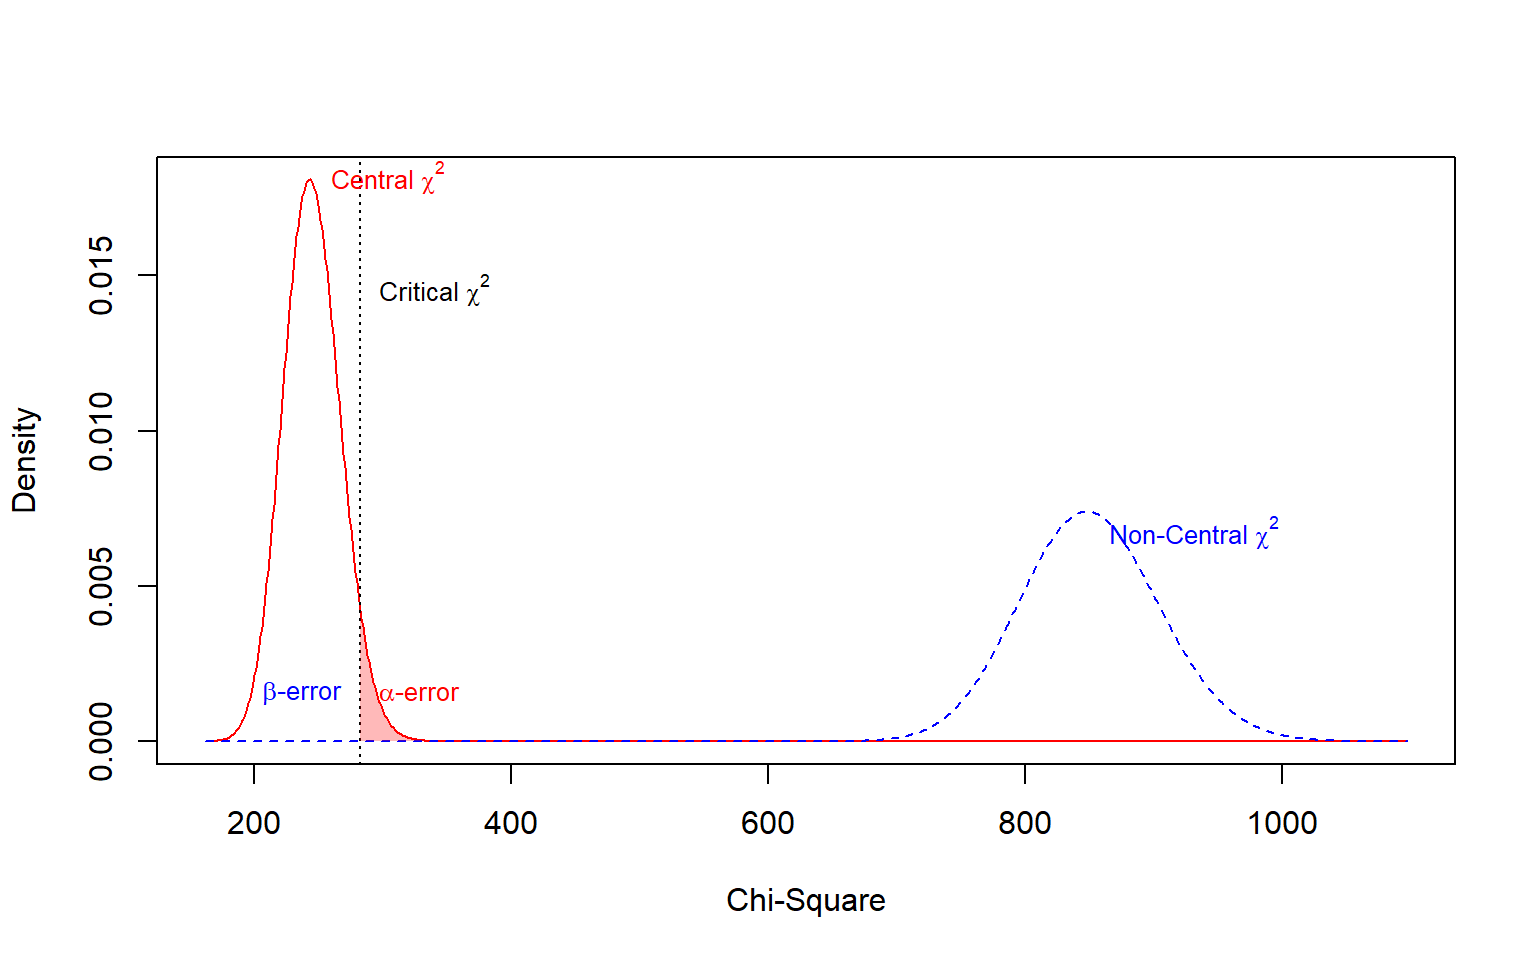
\includegraphics[keepaspectratio]{index_files/figure-latex/Scripts-AnalysisScripts-06_posthoc-fig-posthoc-realmodel-output-1.png}}

}

\caption{\label{fig-posthoc-realmodel}Post hoc power analysis for the
real model.}

\end{figure}%

\textsubscript{Source:
\href{https://phdpablo.github.io/cfa-power/Scripts/AnalysisScripts/06_posthoc-preview.html\#cell-fig-posthoc-realmodel}{Post
Hoc Power Analysis}}

However, post hoc power must always be interpreted with methodological
caution. Calculating power retrospectively from observed sample
statistics after finding a non-significant result constitutes the
well-known ``observed power fallacy'' (Jobst et al., 2023; MacCallum et
al., 1996; Zhang \& Yuan, 2018), where low power is simply a
tautological re-expression of an unremarkable \(p\)-value. Post hoc
power analysis remains legitimate only when framed
prospective-retrospectively: asking whether the collected \(N\)
possessed adequate sensitivity to reject a pre-specified, theoretically
grounded alternative (\(H_1\)) that was determined prior to inspecting
data-derived effects (Moshagen \& Bader, 2024; Wang, 2023).

\section*{References}\label{references}
\addcontentsline{toc}{section}{References}

\protect\phantomsection\label{refs}
\begin{CSLReferences}{1}{0}
\bibitem[\citeproctext]{ref-aguirre-urreta2024}
Aguirre-Urreta, M. I., Rönkkö, M., \& McIntosh, C. N. (2024). Too
{Small} to {Succeed}: {Small Samples} and the p-{Value Problem}.
\emph{SIGMIS Database}, \emph{55}(3), 12--49.
\url{https://doi.org/10.1145/3685235.3685238}

\bibitem[\citeproctext]{ref-buchberger2024}
Buchberger, E. S., Ngo, C. T., Peikert, A., Brandmaier, A. M., \&
Werkle-Bergner, M. (2024). Estimating statistical power for structural
equation models in developmental cognitive science: {A} tutorial in {R}.
\emph{Behavior Research Methods}, \emph{56}(7), 1--18.
\url{https://doi.org/10.3758/s13428-024-02396-2}

\bibitem[\citeproctext]{ref-feng2023}
Feng, Y., \& Hancock, G. R. (2023). Power {Analysis} within a
{Structural Equation Modeling Framework}. In R. H. Hoyle (Ed.),
\emph{Handbook of {Structural Equation Modeling}}. The Guilford Press.

\bibitem[\citeproctext]{ref-irmer2024}
Irmer, J. P., Klein, A. G., \& Schermelleh-Engel, K. (2024).
Model-implied simulation-based power estimation for correctly specified
and distributionally misspecified models: Applications to nonlinear and
linear structural equation models. \emph{Behavior Research Methods},
\emph{56}(8), 8955--8991.
\url{https://doi.org/10.3758/s13428-024-02507-z}

\bibitem[\citeproctext]{ref-jak2021}
Jak, S., Jorgensen, T. D., Verdam, M. G. E., Oort, F. J., \& Elffers, L.
(2021). Analytical power calculations for structural equation modeling:
{A} tutorial and {Shiny} app. \emph{Behavior Research Mehods},
\emph{53}, 1385--1406.
\url{https://doi.org/10.3758/s13428-020-01479-0/Published}

\bibitem[\citeproctext]{ref-jobst2023}
Jobst, L. J., Bader, M., \& Moshagen, M. (2023). A tutorial on assessing
statistical power and determining sample size for structural equation
models. \emph{Psychological Methods}, \emph{28}(1), 207--221.
\url{https://doi.org/10.1037/met0000423}

\bibitem[\citeproctext]{ref-kyriazos2018}
Kyriazos, T. A. (2018). Applied {Psychometrics}: {Sample Size} and
{Sample Power Considerations} in {Factor Analysis} ({EFA}, {CFA}) and
{SEM} in {General}. \emph{Psychology}, \emph{09}(08), 2207--2230.
\url{https://doi.org/10.4236/psych.2018.98126}

\bibitem[\citeproctext]{ref-liang2024}
Liang, A., \& Sterba, S. K. (2024). Power analysis to detect misfit in
{SEMs} with many items: Resolving unrecognized problems, relating old
and new approaches, and {``matching''} power analysis approach to data
analysis approach. \emph{Psychological Methods}.
\url{https://doi.org/10.1037/met0000684}

\bibitem[\citeproctext]{ref-lin2022}
Lin, L.-C., \& Yao, G. (2022). Validation of the factor structure of the
{WHOQOL-BREF} using meta-analysis of exploratory factor analysis and
social network analysis. \emph{Psychological Assessment}, \emph{34}(7),
660--670. \url{https://doi.org/10.1037/pas0001122}

\bibitem[\citeproctext]{ref-maccallum1996}
MacCallum, R. C., Browne, M. W., \& Sugawara, H. M. (1996). Power
analysis and determination of sample size for covariance structure
modeling. \emph{Psychological Methods}, \emph{1}(2), 130--149.
\url{https://doi.org/10.1037/1082-989X.1.2.130}

\bibitem[\citeproctext]{ref-mcneish2021}
McNeish, D., \& Wolf, M. G. (2021). Dynamic fit index cutoffs for
confirmatory factor analysis models. \emph{Psychological Methods},
\emph{28}(1), 61--88. \url{https://doi.org/10.1037/met0000425}

\bibitem[\citeproctext]{ref-moshagen2024}
Moshagen, M., \& Bader, M. (2024). {semPower}: {General} power analysis
for structural equation models. \emph{Behavior Research Methods},
\emph{56}(4), 2901--2922.
\url{https://doi.org/10.3758/s13428-023-02254-7}

\bibitem[\citeproctext]{ref-mosqueirataipe2026}
{Mosqueira Taipe, C. M., Amador Campos, J. A., Krieger, V., Miasso, A.
I., Molina, N. P. F. M., \& dos Santos, P. L.} (2026). Systematic review
of the factor structure of {WHOQOL-bref} in adult population.
\emph{Quality of Life Research}, \emph{35}(17), 1--18.
\url{https://doi.org/10.1007/s11136-025-04115-6}

\bibitem[\citeproctext]{ref-muthen2002a}
Muthén, L. K., \& Muthén, B. O. (2002). How to {Use} a {Monte Carlo
Study} to {Decide} on {Sample Size} and {Determine Power}.
\emph{Structural Equation Modeling: A Multidisciplinary Journal},
\emph{9}(4), 599--620. \url{https://doi.org/10.1207/S15328007SEM0904_8}

\bibitem[\citeproctext]{ref-simsem2021}
Pornprasertmanit, S., Miller, P., Schoemann, A., \& Jorgensen, T. D.
(2021). \emph{Simsem: {SIMulated Structural Equation Modeling}}.
\url{https://CRAN.R-project.org/package=simsem}

\bibitem[\citeproctext]{ref-rogers2022}
Rogers, P. (2022). Best {Practices} for {Your Exploratory Factor
Analysis}: {A Factor Tutorial}. \emph{Revista de Administração
Contemporânea}, \emph{26}(6).
\url{https://doi.org/10.1590/1982-7849rac2022210085.en}

\bibitem[\citeproctext]{ref-schoemann2014}
Schoemann, A. M., Miller, P., Pornprasertmanit, S., \& Wu, W. (2014).
Using {Monte Carlo} simulations to determine power and sample size for
planned missing designs. \emph{International Journal of Behavioral
Development}, \emph{38}(5), 471--479.
\url{https://doi.org/10.1177/0165025413515169}

\bibitem[\citeproctext]{ref-wang2023}
Wang, Y. A. (2023). \emph{How to {Conduct Power Analysis} for
{Structural Equation Models}: {A Practical Primer}} {[}Preprint{]}.
PsyArXiv. \url{https://doi.org/10.31234/osf.io/4n3uk}

\bibitem[\citeproctext]{ref-wang2021}
Wang, Y. A., \& Rhemtulla, M. (2021). Power {Analysis} for {Parameter
Estimation} in {Structural Equation Modeling}: {A Discussion} and
{Tutorial}. \emph{Advances in Methods and Practices in Psychological
Science}, \emph{4}(1), 1--17.
\url{https://doi.org/10.1177/2515245920918253}

\bibitem[\citeproctext]{ref-wolf2013}
Wolf, E. J., Harrington, K. M., Clark, S. L., \& Miller, M. W. (2013).
Sample {Size Requirements} for {Structural Equation Models}: {An
Evaluation} of {Power}, {Bias}, and {Solution Propriety}.
\emph{Educational and Psychological Measurement}, \emph{76}(6),
913--934. \url{https://doi.org/10.1177/0013164413495237}

\bibitem[\citeproctext]{ref-zhang2018}
Zhang, Z., \& Yuan, K.-H. (2018). \emph{Practical statistical power
analysis using {Webpower} and {R}}. ISDSA Press.

\end{CSLReferences}




\end{document}
